 %\documentclass[lettersize,journal]{IEEEtran}
\documentclass[10pt,journal,compsoc]{IEEEtran}
\usepackage{amsmath,amsfonts}
\usepackage{algpseudocode}
\usepackage{algorithm}
\usepackage{enumitem}
\usepackage{array}
%\usepackage[caption=false,font=normalsize,labelfont=sf,textfont=sf]{subfig}
\usepackage{textcomp}
%\usepackage{stfloats}
\usepackage{url}
\usepackage{verbatim}
\usepackage{graphicx}
\usepackage{cite}
\usepackage[numbers]{natbib}
\usepackage[hidelinks]{hyperref}
\usepackage{caption}
\usepackage{color}
\usepackage{tabularray}
\usepackage{subcaption}
\usepackage{multirow}
\usepackage{colortbl}
\usepackage{adjustbox}
\usepackage{subcaption}
\usepackage{booktabs}
%\usepackage[section]{placeins}
\definecolor{Black}{RGB}{0,0,0}
\hyphenation{op-tical net-works semi-conduc-tor IEEE-Xplore}
\UseTblrLibrary{diagbox}
\renewcommand\thesubfigure{\arabic{subfigure}}
% updated with editorial comments 8/9/2021

%\floatsetup[table]{capposition=top,captionskip=0pt,} % 将caption位于表格上方

\captionsetup[table]{labelsep=newline, font=bf}
\captionsetup[figure]{font=footnotesize,labelfont=sf,textfont=sf,font=sf,justification=raggedright, singlelinecheck=false}
\captionsetup[subfigure]{justification=centering}

\def\figureautorefname{Fig.}%使用Fig.引用表格
\makeatletter
\g@addto@macro{\UrlBreaks}{\do\/\do-}
\makeatother


\begin{document}

%\title{A Sample Article Using IEEEtran.cls\\ for IEEE Journals and Transactions}
\title{Multi-party Federated Recommendation \\ Based on Semi-supervised Learning}
\author
	{
	Xin Liu, Jiuluan Lv, Feng Chen, Qingjie Wei, Hangxuan He, Ying Qian
	\thanks{
		Xin Liu, Jiuluan Lv, Feng Chen, Qingjie Wei, Hangxuan He and Ying Qian are with the School of Software Engineering, Chongqing University of Posts and Telecommunications, 400065, Chongqing, China. \\
		E-mails: liuxin@cqupt.edu.cn, s221201028@stu.cqupt.edu.cn, chenfeng@cqupt.edu.cn, weiqj@cqupt.edu.cn, s221231019@stu.cqupt.edu.cn, qianying@cqupt.edu.cn \\
		Corresponding author: Ying Qian
		}
	}
%\author{Xin Liu, Jiuluan Lv, Feng Chen, Qingjie Wei, Hangxuan He, Ying Qian\thanks{Corresponding author: Ying Qian}}
%\IEEEcompsocitemizethanks{
%	\IEEEcompsocthanksitem Xin Liu, Jiuluan Lv, Feng Chen, Qingjie Wei, Hangxuan He and Ying Qian are with the School of Software Engineering, Chongqing University of Posts and Telecommunications, 400065, Chongqing, China. E-mails: liuxin@cqupt.edu.cn, s221201028@stu.cqupt.edu.cn, chenfeng@cqupt.edu.cn, weiqj@cqupt.edu.cn, s221231019@stu.cqupt.edu.cn, qianying@cqupt.edu.cn}
% The paper headers
\markboth{Journal of IEEE Transactions on Big Data}%
{Xin Liu, Jiuluan Lv, \MakeLowercase{\textit{et al.}}: A Sample Article Using IEEEtran.cls for IEEE Journals}

%\IEEEpubid{0000--0000/00\$00.00~\copyright~2021 IEEE}
% Remember, if you use this you must call \IEEEpubidadjcol in the second
% column for its text to clear the IEEEpubid mark.

\IEEEtitleabstractindextext{%
	\begin{abstract}
	Leveraging multi-party data to provide recommendations remains a challenge particularly when the party in need of recommendation services possesses only positive samples while other parties just have unlabeled data. To address UDD-PU learning problem, this paper proposes an algorithm VFPU, Vertical Federated learning with Positive and Unlabeled data. VFPU conducts random sampling repeatedly from the multi-party unlabeled data, treating sampled data as negative ones. It hence forms multiple training datasets with balanced positive and negative samples, and multiple testing datasets with those unsampled data. For each training dataset, VFPU trains a base estimator adapted for the vertical federated learning framework iteratively. We use the trained base estimator to generate forecast scores for each sample in the testing dataset. Based on the sum of scores and their frequency of occurrence in the testing datasets, we calculate the probability of being positive for each unlabeled sample. Those with top probabilities are regarded as reliable positive samples. They are then added to the positive samples and subsequently removed from the unlabeled data. This process of sampling, training, and selecting positive samples is iterated repeatedly. Experimental results demonstrated that VFPU performed comparably to its non-federated counterparts and outperformed other federated semi-supervised learning methods.
	\end{abstract}
	
	% Note that keywords are not normally used for peerreview papers.
\begin{IEEEkeywords}
	Recommendation Method, Vertical Federated Learning, Semi-supervised Learning, Positive and Unlabeled Learning
\end{IEEEkeywords}

}

\maketitle






\section{Introduction}
\IEEEPARstart{R}{ecommendation} systems are crucial in various real-world business areas, such as e-commerce \cite{sarwar2000analysis,schafer2001commerce}, news \cite{zheng2018drn,liu2010pedersen}, and healthcare \cite{kim2014item,yue2021overview}. These systems generally incorporate machine learning models to generate recommendations. Training the model requires extensive data, including sensitive information, such as users' personal information, user behaviours, social relations, and contextual data, e.g. the current location/time/activity. In order to achieve high accuracy, most recommendation systems store the data on a central server. However, this can result in significant privacy risks, such as theft, loss and unauthorized use of data. Furthermore, due to regulatory restrictions and in situations where data are proprietary and owned by different parties, it becomes increasingly challenging and even impossible to develop recommendation systems with data centrally integrated across multiple parties.

Federated learning (FL) is a distributed learning approach introduced by Google \cite{mcmahan2017communication} and provides a promising solution for privacy-preserving recommendation systems. FL allows different data owners (clients) to cooperatively train machine learning models by sharing intermediate parameters, such as model parameters and gradients, instead of sharing raw data. Current FL research primarily addresses problems with fully labeled data using supervised learning. However, many real-world problems lack fully labeled data, and fully labeling the data is challenging due to factors such as a shortage of domain expertise, resource constraints, or the absence of proper labeling tools. Therefore, in recent years there have been some research efforts that use semi-supervised learning to address FL problems with limited labeled data, especially for problems involving only Positive and Unlabeled data, which are called PU problems.

\citet{lin2022federated} proposed FedPU algorithm to address the PU problem in the federated setting where each client only labels a little part of their dataset. \citet{liang2022rscfed} presented RSCFed, which addresses the uneven reliability of non-independent and identically distributed (Non-IID) local clients by updating the global model via aggregating multiple sub-consensus models. \citet{jeong2020federated} proposed FedMatch algorithm to optimize inter-client consistency and parameter decomposition for effective learning with limited labeled data. \citet{wang2022enhancing} presented AdaFedSemi, which leverages on-device labeled data and in-cloud unlabeled data, using a multi-armed bandit-based algorithm to optimize client participation and pseudo-label quality. However, all of these works focus on scenarios in which all parties share the same feature space, which is also known as Horizontal Federated Learning (HFL) \cite{yang2019federated}. There is research gap in applying semi-supervised techniques in the scenario where all parties share the same sample ID space; but differ in the feature space, which is also known as Vertical Federated Learning (VFL) \cite{yang2019federated}.

In this paper, we explore a VFL scenario with the following characteristics: 1) Multiple parties maintain proprietary datasets with partially overlapping sample IDs but distinct feature spaces; 2) The party in need of the recommendation service possesses data containing only positive samples, while the other parties have unlabeled data; 3) All parties aim to jointly train a recommendation model to identify reliable positive samples from the unlabeled data.

Notably, the second characteristic mentioned above corresponds to the problem of learning from positive and unlabeled (PU) data. PU methods \cite{mordelet2014bagging,liu2003building,liu2015classification,xu2017multi} are designed to effectively leverage unlabeled samples to address  the PU problem. However, it is a new challenge when one party possesses only positive samples and has no access to the unlabeled samples held by other parties. We refer to this as the Unlabeled-Data-Deficient PU (UDD-PU) learning problem. In other words, conventional PU learning frameworks alone cannot address this issue.

This paper proposes the Vertical Federated Learning with Positive and Unlabeled data (VFPU) algorithm that enables multiple parties to cooperatively train a machine learning model to identify reliable positive samples within unlabeled data. Our primary contributions are as follows:
\begin{itemize}
	\item We identify the UDD-PU learning problem in the context of vertical federated learning that has not been adequately explored in the existing literature.
	\item We propose the VFPU algorithm and present a recommendation solution to address the UDD-PU learning problem, enabling multiple parties to  collaboratively train a machine learning model while preserving privacy.
	\item We demonstrate that VFPU can perform comparably to its non-federated counterparts and outperform other federated semi-supervised learning methods. Therefore, the recommendation solution proposed based on VFPU can effectively address the challenge posed by the UDD-PU learning problem.
\end{itemize}

This paper is organized as follows: Section \ref{sec2} discusses related work on federated learning and semi-supervised learning. Then, we present the problem formulation and the recommendation method based on VFPU in Section \ref{sec3}. Experimental results are presented in Section \ref{sec4}, followed by a conclusion in Section \ref{sec5}.  


\section{Related Work}
\label{sec2}
\subsection{Federated Learning}
Federated learning (FL), initially proposed by \citet{mcmahan2017communication}, was developed to facilitate a collaborative model learning without the need to collect data from participating individuals. This approach involves training local models on local data with a consistent model architecture, updating the global model by averaging all local models, and avoiding data transmission by conducting model training on individual mobile terminals \cite{konevcny2016federated,bonawitz2017practical,kairouz2021advances}. Building on this idea, researchers have adapted various machine learning models for the federated setting, including decision trees \cite{zhao2018inprivate,li2020practical}, linear/logistic regression \cite{li2020federated,hanzely2020lower,mohri2019agnostic}, and neural networks \cite{yurochkin2019bayesian,wang2020federated}.

\citet{bonawitz2017practical} introduced secure aggregation based on the Secure Multiparty Computation (SMC) to enhance the security of federated learning. This method allows for aggregating private values from multiple mutually distrustful parties without revealing any information about their individual private values. Additionally, \citet{geyer2017differentially} incorporated client-level differential privacy to safeguard privacy further, preventing clients from attempting to reconstruct another client's private data by exploiting the global model. Differential privacy \cite{dwork2008differential} and k-anonymity \cite{sweeney2002k} are techniques employed by another line of work for data privacy protection. Homomorphic encryption (HE) \cite{rivest1978data} is utilized to safeguard user data privacy by enabling parameter exchange under the encrypted mechanism.

The concept of vertical federated learning (VFL) was first introduced in \cite{yang2019federated,hardy2017private}, with protocols proposed for linear models \cite{hardy2017private,liu2019communication} and neural networks \cite{liu2020secure}. Prior works have also explored privacy-preserving decision trees for vertically partitioned data \cite{vaidya2008privacy}. In another study, \citet{djatmiko2017privacy} proposed jointly running logistic regression on encrypted, vertically-partitioned data by approximating a non-linear logistic loss using a Taylor expansion, which may inevitably affect the model's performance. Gradient Boosted Decision Trees (GBDT) \cite{friedman2001greedy} is a widely-used ensemble learning method in machine learning and data science. Various GBDT-based VFL algorithms have been proposed in the literature, including SecureBoost \cite{cheng2021secureboost}, SecureBoost+ \cite{chen2021secureboost+}, and SecureGBM \cite{feng2019securegbm}. These algorithms utilize additive homomorphic encryption (HE) to protect residual errors and feature histograms transmitted between active and passive parties during the learning process. Private Set Intersection (PSI) is widely used to ensure privacy-preserving entity alignment in VFL. A PSI protocol enables parties to collectively determine the common ID intersection without divulging any extra information. Implementation of PSI protocols can be achieved through several techniques, such as encryption and signature strategies \cite{liang2004privacy}, and oblivious transfer \cite{pinkas2014faster,pinkas2018scalable}.  

\subsection{Semi-supervised Learning}
Semi-supervised learning (SSL) is a machine learning approach that uses a combination of labeled and unlabeled data to train a model. Despite the extensive research in SSL, our focus primarily centers on the Positive-Unlabeled (PU) learning method, a particular type of SSL approach specializing in the standard semi-supervised setting. In PU learning, various algorithms and techniques have been proposed to address the challenges posed by this learning scenario, where a learner has access only to positive examples and unlabeled data. One such approach is the two-step technique proposed by \citet{liu2003building}, which leverages the assumption that positive samples are similar to labeled examples while negative samples are substantially different. This method involves identifying reliable negative examples and, optionally, generating additional positive examples. Another category of algorithms for PU learning is biased PU learning methods, which treat unlabeled examples as negative examples with class label noise. For instance, \citet{liu2015classification} introduced a method that regarded the unlabeled samples as negative ones with label noise, while \citet{liu2003building} considered the unlabeled data as negative examples with smaller weights and performed logistic regression after weighting the samples.

The presence of noise in the negative data complicates the learning process, because it may assign too much importance to a negative example that is, in fact, positive. To address this issue, various techniques have been proposed, such as bagging and least-square SVMs (LS-SVM) \cite{suykens1999least}. Bagging SVM is a technique that trains multiple biased SVM classifiers, each on the positive examples and a subset of the negative examples. This approach has been further extended by \citet{mordelet2014bagging}, who builds upon bagging SVMs by resampling both the positive and negative examples and employing a bootstrap strategy to improve performance.

\section{Proposed Approach}
\label{sec3}
	In this section, we elaborate on the setup of the Unlabeled-Data-Deficient PU (UDD-PU) learning problem and the proposed algorithm, namely vertical federated learning with positive and unlabeled data (VFPU). We demonstrate how the VFPU algorithm can be used to provide recommendation solution to the UDD-PU learning problem.
\subsection{Problem Setup}
Firstly, consider a scenario with $K$ data owners and one central server. Let matrix ${{\mathsf{\mathcal{D}}}_{k}}$ represent the data held by the $k\text{-th}$ data owner, where each row of the matrix represents a sample, and each column represents a feature. The dataset can be represented as $(\mathsf{\mathcal{I}}\text{,}\mathsf{\mathcal{X}}\text{,}\mathsf{\mathcal{Y}})$, where $\mathsf{\mathcal{I}}$  denotes the samples' ID space, $\mathsf{\mathcal{X}} $ denotes the feature space, and $\mathsf{\mathcal{Y}}$ denotes the label space. In the traditional vertical federated learning (VFL) setting, at least one party possesses complete labels of its dataset. However, obtaining fully labeled data in many real-world scenarios is challenging due to business constraints.

For the purpose of illustration, let us consider a scenario involving three data owners: party A, party B, and party C. These data owners possess sensitive data and need to collaborate securely while maintaining data privacy. Suppose there are two classes of samples, namely positive and negative. All three parties share some overlap on sample IDs. Let $P$  represent the collection of positive samples owned by party A, which contains only positive data. Let $U$  denote the collection of unlabeled data held by party B and party C, except for those already contained in party A. The three parties aim to jointly train a recommendation model to identify reliable positive samples from $U$, as the true labels in $U$  are unknown. Let $R$  represent the collection of reliable positive samples identified by the model. Therefore, with this model, $R$ can be provided to party A for relevant product recommendations. 

In this problem setting, conventional vertical federated learning algorithms cannot be directly applied since none of the clients holds complete labels. One possible approach is to apply semi-supervised learning techniques, such as PU learning. However, traditional PU learning methods require both $P$  and  $U$ at the same time, whereas in the given scenario, party A only possesses $P$. 

As a result, for party A, who wants to incorporate recommendation services for its business, there is an Unlabeled-Data-Deficient PU (UDD-PU) learning recommendation problem, which cannot be directly addressed by existing methods. 

	\subsection{Recommendation Based on VFPU}To tackle the UDD-PU learning problem, we propose the VFPU algorithm, which combines a vertical federated learning framework with PU learning techniques. VFPU addresses the issue of Party A's insufficient unlabeled samples and enhances the recommendation model's performance. 

In this paper, the recommendation process based on the VFPU includes three primary steps: data preprocessing, encrypted sample alignment, and the execution of the VFPU algorithm. The primary goal of VFPU is to identify reliable positive samples within the unlabeled dataset. These samples allow the model to gain a deeper understanding of positive instance attributes, resulting in more accurate and personalized product recommendations for Party A. Simultaneously, we ensure data privacy and collaboration among multiple parties. \autoref{fig:VFPU} illustrates the recommendation process. The detailed steps in the process will be elaborated in the following sections.
\begin{figure*}[!htbp]
	\centering
%	\captionsetup{font=scriptsize}
	\captionsetup{size=footnotesize}
%tiny scriptsize footnotesize small normalsize large Large LARGE huge Huge
	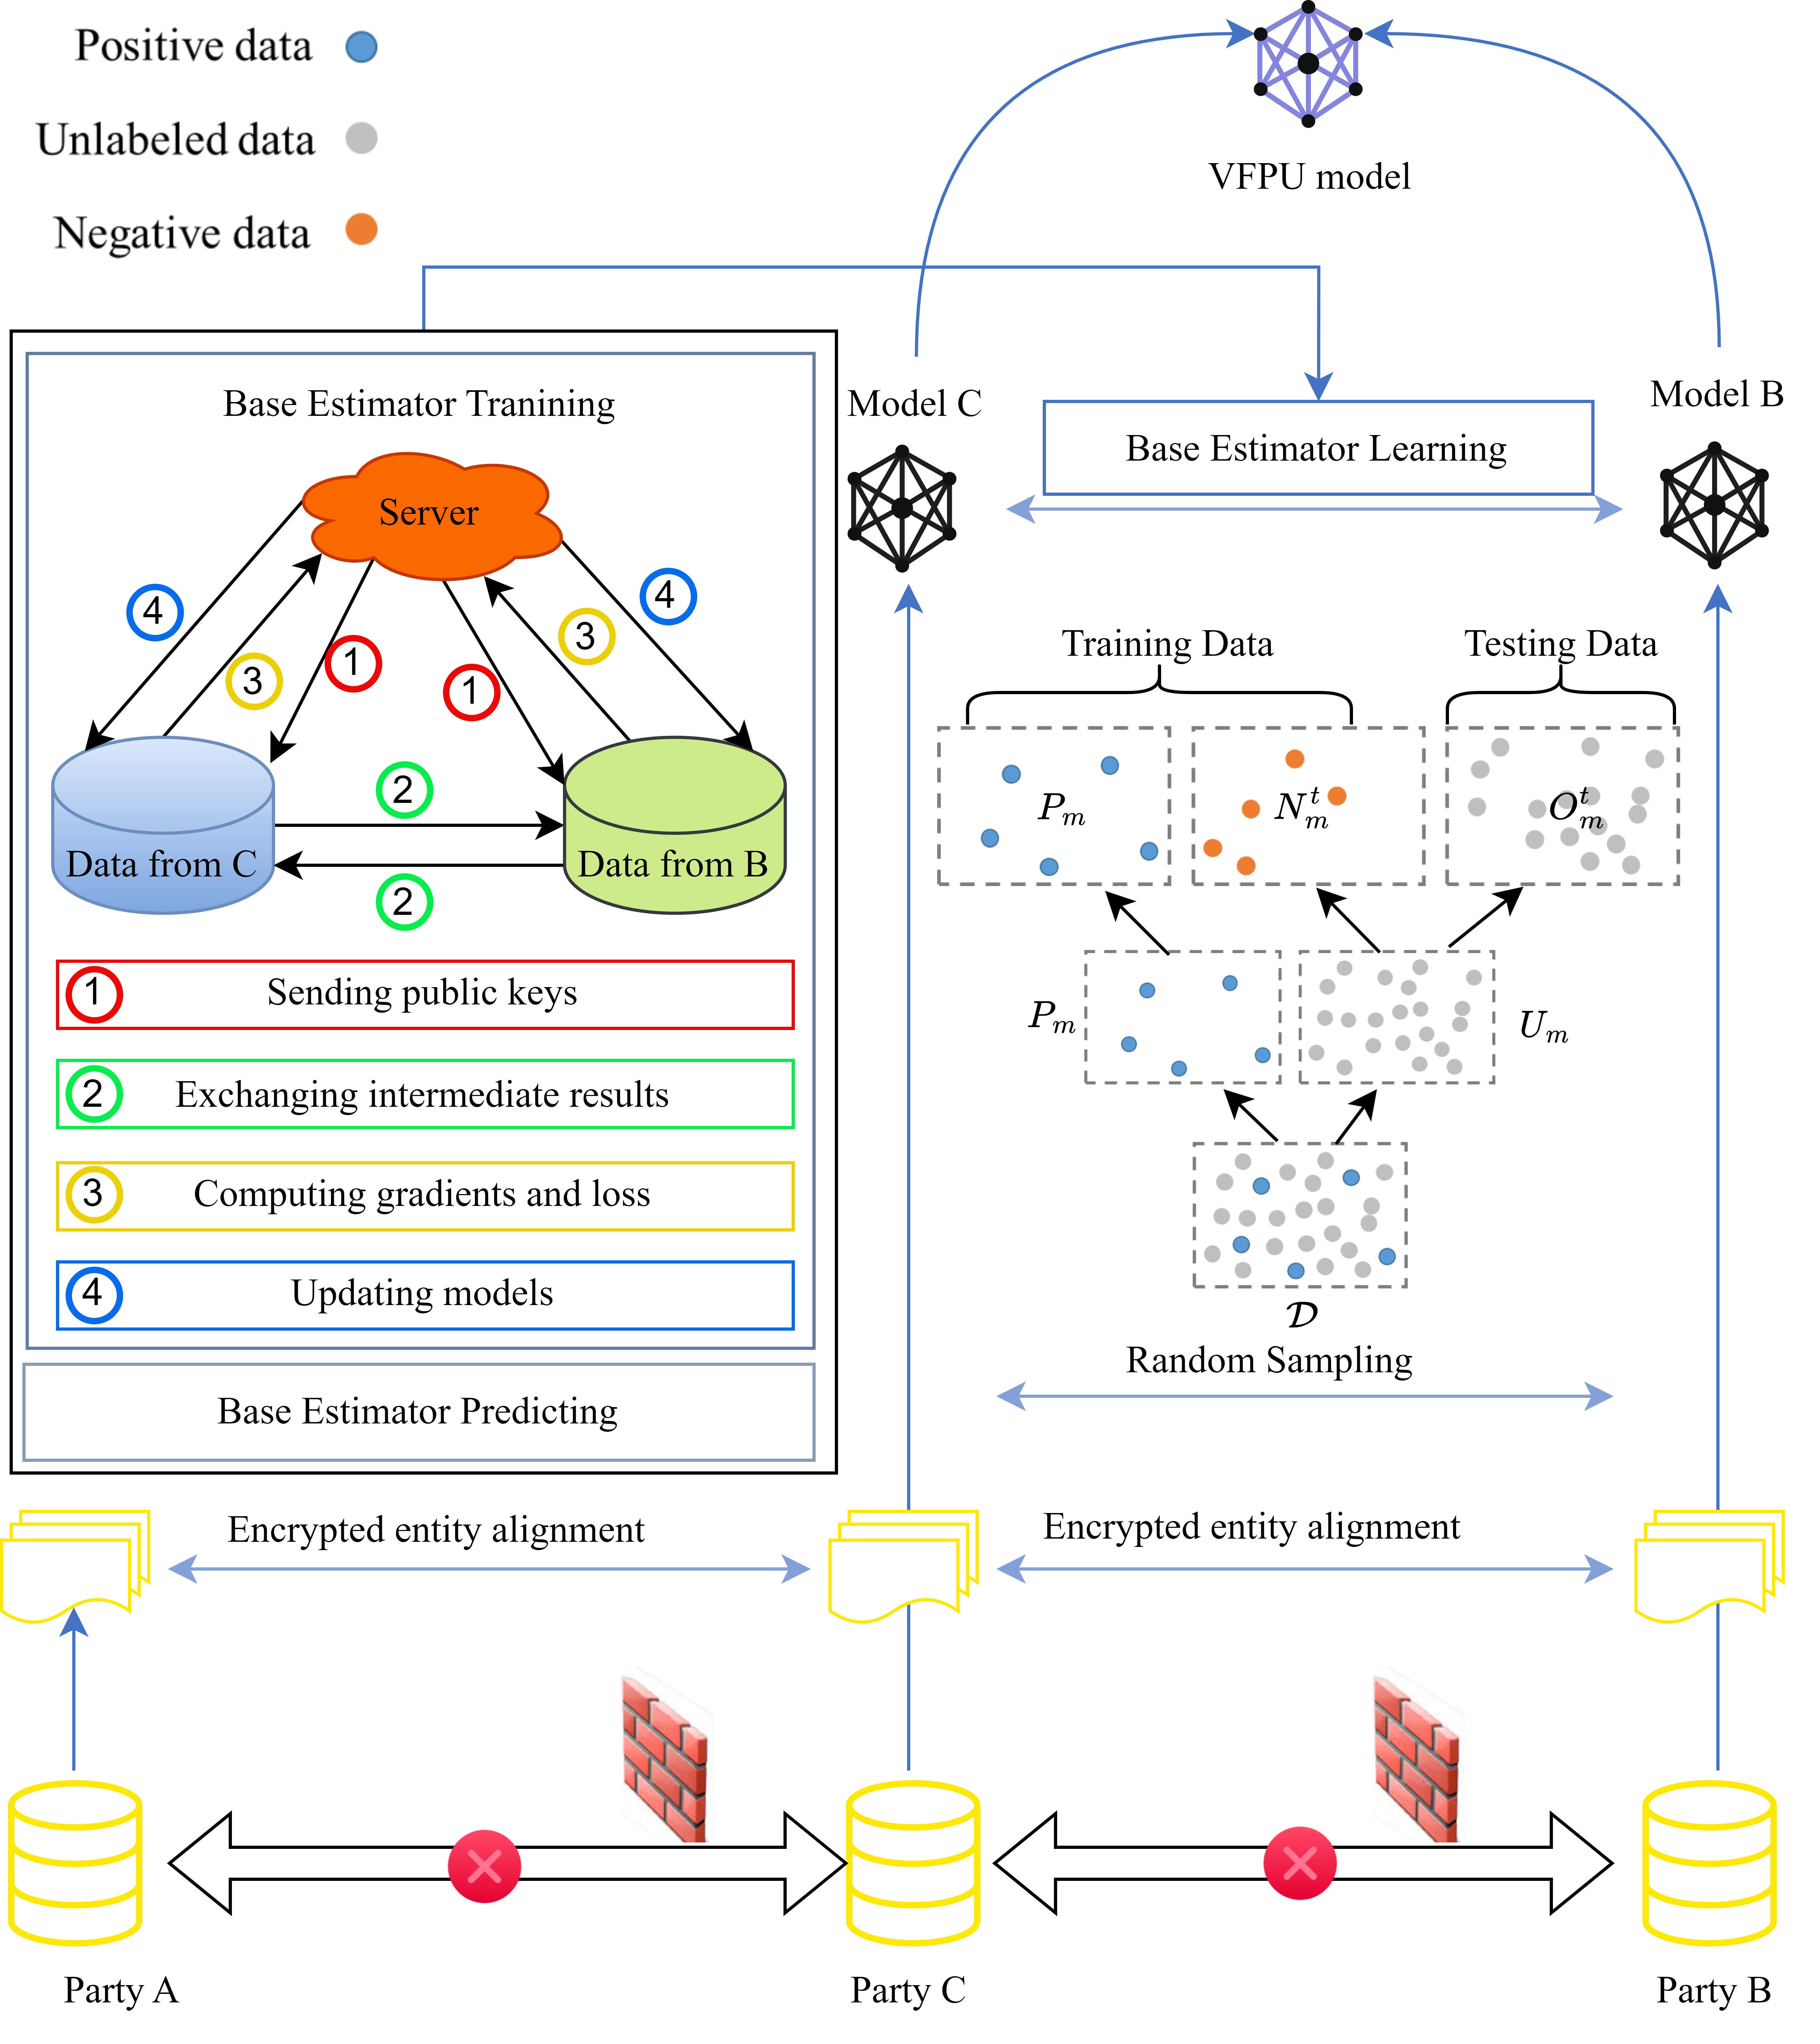
\includegraphics[width=0.9\textwidth]{./Figure 1 in JEPG format}
	\caption{The overall process of the proposed VFPU algorithm.}
	\label{fig:VFPU}
\end{figure*}
\subsubsection{Data preprocessing and encrypted sample alignment}
\begin{enumerate}[label=(\arabic*)]
	\item Data preprocessing
	
	We apply various preprocessing techniques to the data held by parties A, B, and C, including data cleaning, normalization, and feature encoding. Categorical features are handled using one-hot encoding, while numerical features are normalized using standardized scaling.
	\item Encrypted sample alignment
	
	After data preprocessing, the three parties securely perform the sample alignment process in the following two steps:
	\begin{itemize}
		\item Step 1: Party B and party C align their sample ID spaces, retaining only the samples that both parties share and discarding the unaligned ones respectively. As a result, party B and party C now share the same samples but different features.
		\item Step 2: Party A and party C align their sample ID spaces without removing any samples. Aligned samples are those that appear in both parties’ datasets. Based on the alignment, aligned samples in party C are assigned with the label of 1, indicating positive samples. Meanwhile, unaligned samples in party C receive a label of -1, indicating unlabeled samples.
	\end{itemize}
\end{enumerate}


After the encrypted sample alignment, party C holds both positive and unlabeled samples. This process effectively transforms the UDD-PU recommendation problem into a vertical federated training scenario with the PU prohlem between party B and party C. 

To protect data privacy during the sample alignment process, we utilize the Blind RSA-based Private Set Intersection (PSI) protocol \cite{de2010practical}. This protocol enables all parties to securely compute the intersection of their datasets without revealing any additional information about the samples they hold. With the completion of these tasks, the datasets are now ready for the execution of the VFPU algorithm.

\subsubsection{Vertical federated learning with positive and unlabeled data}
The objective of the VFPU algorithm is to securely and efficiently identify reliable positive samples from the unlabeled data. The core of the algorithm lies in the combination of some PU learning techniques with the vertical federated framework. The PU techniques incorporated in VFPU include the two-step technique \cite{liu2003building} and the PU bagging method \cite{mordelet2014bagging}. This section provides a detailed explanation of VFPU, as outlined in Algorithm \ref{alg:cap}. 



\begin{enumerate}[label=(\arabic*)]
	\item Establishing initial sample sets
	
	Overall, the VFPU algorithm executes $M$ iterations, each consisting of $T$ rounds of random sampling, training and predicting.  In each iteration $m\in \{1,...,M\}$, the set of positive samples ${{P}_{m}}$ and the set of unlabeled samples ${{U}_{m}}$ are determined based on the labels provided by Party C as follows:
	\begin{equation}
		\begin{split}
			&{{P}_{m}}=\{i|\mathsf{\mathcal{Y}}_{i}^{C}=1,\ i\in {{\mathsf{\mathcal{I}}}_{C}}\};\\
			&{{U}_{m}}=\{i|\mathsf{\mathcal{Y}}_{i}^{C}=-1,\ i\in {{\mathsf{\mathcal{I}}}_{C}}\},
		\end{split}
	\end{equation}
	where ${{\mathsf{\mathcal{I}}}_{C}}$ is the ID space, ${{\mathsf{\mathcal{Y}}}^{C}}$ is the label space of party C, and $i$ is the sample ID.
	\item Sampling, training and predicting
	
	As shown in \autoref{fig:VFPU}, during the $t\text{-th} \ (\text{t}\in \{1,2,...,T\})$ round of sampling in the $m\text{-th}$ iteration, a pseudo-negative sample set $N_{m}^{t}$ is generated from ${{U}_{m}}$ using bootstrapping \cite{mordelet2014bagging}. Mathematically, this can be expressed as:
	\begin{equation}
		%				\small
		N_{m}^{t}=\{ \text{Randomly select} \ |P_{m}| \ \text{elements from} \ U_{m} \},
	\end{equation}
	where $|{{P}_{m}}|$ is the number of samples as contained in ${{P}_{m}}$.
	
	Since the actual categories of the unlabeled samples are unknown, $N_{m}^{t}$ is regarded as a set of pseudo-negative samples, potentially containing both genuine negative and positive samples. By drawing $|{{P}_{m}}|$ elements from ${{U}_{m}}$, we can create $N_{m}^{t}$ with the same size as ${{P}_{m}}$.
	
	${{P}_{m}}$ and $N_{m}^{t}$ are combined into a binary classification training set during the training process. This set is used to train the vertical federated learning model, which learns to distinguish between positive and negative samples and applies this knowledge to future prediction tasks. 
	
	Bootstrapping is a technique that randomly selects samples from a dataset with replacement. Employing this technique allows VFPU to create diverse and balanced training sets, thus improving the model's generalization capabilities, reducing potential biases and enhancing the overall performance of the recommendation model.
	
	Samples not selected during the bootstrapping procedure are called out-of-bag samples. The out-of-bag score represents the predicted probability of the out-of-bag sample being classified as positive. Therefore, to obtain the set of out-of-bag samples $O_{m}^{t}$, we need to exclude samples in $N_{m}^{t}$ from ${{U}_{m}}$, which can be expressed mathematically as:
	\begin{equation}
		O_{m}^{t}={{U}_{m}}-N_{m}^{t}.
	\end{equation}
	
	Party C then encrypts and sends   $N_{m}^{t}$,  ${{P}_{m}}$, and $O_{m}^{t}$ t to other parties. Here in our example, the other party is Party B. Then, Party B and Party C establish their training and testing data based on the three sets of sample IDs they have received. Specifically, we have:
	\begin{equation}
		\begin{split}
			&\mathsf{\mathcal{D}}_{train}^{K}=\{(i,{{x}_{i}},{{y}_{i}})|i\in {{P}_{m}}\ or\ i\in N_{m}^{t}\};\\
			&\mathsf{\mathcal{D}}_{test}^{K}=\{(i,{{x}_{i}},{{y}_{i}})|i\in O_{m}^{t}\},
		\end{split}
	\end{equation}
	where $\mathsf{\mathcal{D}}_{train}^{K}$ represents the binary training data and $\mathsf{\mathcal{D}}_{test}^{K}$ denotes the testing data and $K\in \{B,C\}$. ${{x}_{i}}\in \mathsf{\mathcal{X}}$ and ${{y}_{i}}\in \mathsf{\mathcal{Y}}$.
	
	
	Once party B and party C have prepared their respective training and testing datasets, the binary classification problem transforms into a vertical federated training and predicting task. A base estimator, serving as a machine learning model for each party, is adapted for use within the VFL framework. It is crucial to grasp general training process of VFL \cite{yang2019federated}. Overall, it comprises four steps, illustrating how the base estimator is trained on the multi-party training data while preserving privacy. The four steps are as follows:
	\begin{itemize}
		\item Step 1: The server creates encryption pairs and sends a public key to parties B and C.
		\item Step 2: Parties B and C encrypt and exchange intermediate results for gradient and loss calculations.
		\item Step 3: Parties B and C compute encrypted gradients, add an additional mask, and calculate the encrypted loss. Encrypted values are then sent to the server.
		\item Step 4: The server decrypts and sends the decrypted gradients and loss back to party B and party C. Parties B and C unmask the gradients and update the model parameters accordingly.
	\end{itemize}
	
	Various privacy-preserving machine-learning algorithms have been proposed for the VFL framework in support of the general training process \cite{yang2019federated}, including logistic regression (LR) \cite{he2021secure,yang2019parallel}, random forest (RF) \cite{yao2022efficient}, gradient boosting decision tree (GBDT) \cite{he2021secure}, XGBoost (XGB) \cite{xu2021efficient,wang2022feverless} and LightGBM (LGB) \cite{feng2019securegbm}. In this paper, we will apply different base estimators to evaluate the performance of the recommendation model. 
	
	\begin{algorithm}[H]
		\caption{The proposed VFPU algorithm.}
		\label{alg:cap}
		\algrenewcommand\algorithmicrequire{\textbf{Input:}}
		\algrenewcommand\algorithmicensure{\textbf{Output:}}
		\begin{algorithmic}[1]
			\Require Parties $B,C$. Aligned datasets ${{\mathsf{\mathcal{D}}}_{B}}\text{,}{{\mathsf{\mathcal{D}}}_{C}}$  and ID sets ${{\mathsf{\mathcal{I}}}_{B}}\text{,}\ {{\mathsf{\mathcal{I}}}_{C}}$. Maximum number of iterations $M$, number of random sampling iterations $T$ and $\theta$ where $\theta$ is the sampling rate of reliable positive samples.
			\Ensure $R$, a set of reliable positive samples.
			\Procedure{Party C executes}{}
			\For {$m=1,2,\ldots,M$}
			\State ${{P}_{m}}=\{i|\mathsf{\mathcal{Y}}_{i}^{C}=1, \ i\in {{\mathsf{\mathcal{I}}}_{C}}\}$
			\State ${{U}_{m}}=\{i|\mathsf{\mathcal{Y}}_{i}^{C}=-1, \ i\in {{\mathsf{\mathcal{I}}}_{C}}\}$
			\For {$t=1,2,\ldots,T$}
			\State $N_{m}^{t}=\{Randomly\ select\ |{{P}_{m}}|\ elements\ from\ {{U}_{m}} \}$
			\State $O_{m}^{t}={{U}_{m}}-N_{m}^{t}$
			\State Encrypt and send $N_{m}^{t}$, ${P_m}$, and $O_{m}^{t}$ to other parties.
			\State Notify parties to set training data and testing data.
			\State $S_m^t$ = Base\_Estimator\_Learning()
			\EndFor
			\State ${{\mathsf{\mathcal{P}}}_{m}}(u)={\sum\nolimits_{t=1}^{T}{S_{m}^{t}}}(u)/{\sum\nolimits_{t=1}^{T}{I(u\in O_{m}^{t})\text{,}\ \ \forall \text{u}\in }}\;{{U}_{m}}$
			\State ${{R}_{m}}=\{Chose\ Top\ |{{U}_{m}}|\times \theta \ IDs\ from\ {{\mathsf{\mathcal{P}}}_{m}}\}$
			\State $\mathsf{\mathcal{Y}}_{r}^{C}=1\text{,}\ \ \forall r\in {{R}_{m}}$
			\EndFor
			\State $R=\bigcup\limits_{m=1}^{M}{{{R}_{m}}}$
			\EndProcedure
			
			\Function{Base\_Estimator\_Learning}{}():
			\State Server creates encryption pairs, sends public keys to $B$ \& $C$
			\State $B$ \& $C$ encrypt, exchange gradients \& losses.
			\State  $B$ \& $C$ add masks, send encrypted values to server.
			\State Server decrypts, sends back values. $B$ \& $C$ unmask, update models.
			\State \Return Predicted probabilities of positive class on testing data.
			\EndFunction
		\end{algorithmic}
	\end{algorithm}
	
	\item Identifying reliable positive samples
	
	During the $m\text{-th}$ iteration, the process of sampling, training, and predicting is carried out $T$ times. Upon completion of these $T$ rounds, sufficient information is collected to determine the set of probabilities, represented as ${{\mathsf{\mathcal{P}}}_{m}}$, for all unlabeled samples in ${{U}_{m}}$. These probabilities correspond to the likelihood of each sample being regarded as the positive class and can be employed for subsequent decision-making processes, such as pinpointing reliable positive samples and updating training sets.
	
	To derive the entire set ${{\mathsf{\mathcal{P}}}_{m}}$, it is necessary to compute the probability ${{\mathsf{\mathcal{P}}}_{m}}(u)$ for each unlabeled sample $u(u\in {{U}_{m}})$. ${{\mathsf{\mathcal{P}}}_{m}}(u)$ is calculated by summing up the out-of-bag scores of $u$ across all the $T$ rounds and dividing the sum by the total number of occurrences of $u$ remaining as an out-of-bag sample in the $m\text{-th}$ iteration. The subsequent formula can be obtained:
	\begin{equation}
		{{\mathsf{\mathcal{P}}}_{m}}(u)=\frac{\sum\nolimits_{t=1}^{T}{S_{m}^{t}}(u)}{\sum\nolimits_{t=1}^{T}{I(u\in O_{m}^{t})}}.
	\end{equation}
	Note that $S_{m}^{t}(u)$ = 0 if $u$ was not an out-of-bag sample in the $t\text{-th}$ round of sampling during the $m\text{-th}$ iteration. The indicator function $\sum\nolimits_{t=1}^{T}{I(u\in O_{m}^{t})}$ returns 1 if the sample $u$ is in the out-of-bag set $O_{m}^{t}$, and 0 otherwise. 
	
	Based on the probabilities ${{\mathsf{\mathcal{P}}}_{m}}(u)$, we rank all the unlabeled samples decreasingly. Then, the top-ranked samples can be selected as reliable positive samples since they are more probable to be true positive samples. The set of reliable positive samples identified in the $m\text{-th}$ iteration can be denoted as ${{R}_{m}}$ and we have that:
	\begin{equation}
		{{R}_{m}}=\{Chose\ Top\ |{{U}_{m}}|\times \theta \ IDs\ from\ {{\mathsf{\mathcal{P}}}_{m}}\}
	\end{equation}
	This calculation can be performed in two steps:
	\begin{itemize}
		\item Step 1: Sort the samples in ${{\mathsf{\mathcal{P}}}_{m}}$ in a non-increasing order based on their probabilities.
		
		\item Step 2: Select the top $|{{U}_{m}}|\times \theta$ samples from the sorted list, where $\theta $ is a manually set ratio representing the sampling rate of reliable positive samples.
	\end{itemize}
	
	Subsequently, we update the labels of the samples in party C's dataset by adding the selected reliable positive samples to the set of positive samples. As a result, the number of samples in the unlabeled dataset ${{U}_{m}}$ decreasees. Specifically, we can formularize it as follows:
	\begin{equation}
		\mathsf{\mathcal{Y}}_{r}^{C}=1,\ \ r\in {{R}_{m}}
	\end{equation}	
	where each sample $r$ in the set ${{R}_{m}}$ is assigned a label of 1 (positive class).
	\item Final results and application to recommend
	
	After completing all the $M$ iterations of the algorithm, the final set of reliable positive samples $R$ is obtained by taking the union of all ${{R}_{m}}$ sets from each iteration. With this set of reliable positive samples, Party A can now tailor recommendations to each sample in $R$, thereby improving the accuracy and relevance of the recommendation system. This final step is crucial in ensuring the effectiveness of the algorithm in identifying the most relevant samples for enhancing the performance of the recommendation system.
\end{enumerate}
\section{Experiments}
\label{sec4}
In this section, the experimental design and evaluation of the VFPU algorithm are described. First, an overview of the datasets and experimental setup is provided. Following that, a set of research questions to guide the experiment is introduced, and then the experiment results are presented and discussed in terms of each research question.
	\subsection{Experimental Setup}
\textbf{Datasets:} In our experiment, we utilized three datasets to evaluate our proposed method, including the Bank Marketing Dataset\footnote{\label{bank}\url{https://archive.ics.uci.edu/ml/datasets/bank+marketing}}, the Default of Credit Card Clients Dataset\footnote{\sloppy \label{credit}\url{https://www.kaggle.com/uciml/default-of-credit-card-clients-dataset}} and the Adult Census Dataset\footnote{\label{adult}\url{http://archive.ics.uci.edu/ml/datasets/adult}}. The Bank Marketing Dataset is associated with the direct marketing campaigns of a Portuguese banking institution. The marketing campaigns were conducted through phone calls. It comprises four data sets, and we utilized the "bank-additional-full" dataset, which includes a total of 41,188 examples and 20 inputs/features. The data is ordered by date, spanning from May 2008 to November 2010. The classification goal is to predict whether a client will subscribe (yes/no) to a term deposit, represented by the variable "y". The Default of Credit Card Clients Dataset contains data on 30,000 credit card clients and 24 variables, including demographic and payment history information. This dataset is employed to construct predictive models for assessing the likelihood of a client defaulting on loan payments in the following month, indicated by a binary target variable denoting the defaulting status. The Adult Census Dataset is a collection of information about individuals in the United States based on the 1994 Census. It includes details such as age, education,occupation, and income. This dataset is used to predict whether someone earns over \$50,000 per year based on their characteristics. Researchers and machine learning practitioners utilize this dataset to evaluate new models and investigate social patterns related to income and employment. For simplicity, the terms 'Bank', 'Credit', and 'Census' are utilized to represent the three datasets, respectively.

In data preprocessing, categorical features are encoded using one-hot encoding, while numerical features are normalized using standardized scaling.

Each dataset has already been partitioned into training sets and testing datasets by the data provider. We split the data vertically into three parts and distributed them to three parties A, B, and C. We removed the data labels from party B and party C to generate unlabeled data U. For party A, we selected 10\% of the data from the positive class as the positive set P and discarded all the rest of the positive and negative data.

\textbf{Implementation details:} In federated training and prediction of the VFPU algorithm, we used different base estimators to evaluate the performance. Vertical Federated Logistic Regression (VFPU\_LR) was implemented based on \cite{aono2016scalable}. Vertical Federated GBDT (VFPU\_GBDT) and Vertical Federated Random Forest (VFPU\_RF) were realized using the FedTree \cite{li2022fedtree} library. Vertical Federated LightGBM (VFPU\_LGB) was developed using the FATE \cite{liu2021fate} library. To compare the effectiveness of models under federated and non-federated settings, we employed conventional methods to combine all data. The non-federated base estimator counterparts were implemented by various libraries, including LR \cite{pedregosa2011scikit}, GBDT \cite{pedregosa2011scikit}, RF \cite{pedregosa2011scikit}, XGBoost (XGB) \cite{chen2015xgboost}, and LightGBM (LGB) \cite{ke2017lightgbm}. 

To compare different methods, we set the maximum number of iterations $M$ to 5, the sampling rate $\theta$ to 0.02, and the number of random sampling iterations T to 10. We use the Paillier encryption scheme with a key size of 512 bits as our encryption scheme. The default setting specifies a number of parties as 2 \cite{li2022fedtree}. 

\textbf{Evaluation measure:} We used various evaluation measures to assess our proposed method's performance, including accuracy (acc) \cite{liu2003building}, recall  \cite{liu2003building}, precision  \cite{liu2003building}, area under the Receiver Operating Characteristic (ROC) curve (AUC) \cite{cheng2021secureboost}, and F-score (F) \cite{cheng2021secureboost}. The AUC score evaluates the trade-off between the true positive rate and false positive rate. The F-score is the harmonic mean of precision and recall, providing a balanced performance measure.
\subsection{Experimental results}
To investigate the performance of the VFPU algorithm, we introduce three specific research questions (RQs) that guide our evaluation:

RQ1: What is the performance comparison of PU learning with and without federation?

RQ2: What is the impact of different base estimators on VFPU performance, and which one works best?

RQ3: How effective is VFPU at uncovering hidden positive samples compared to other semi-supervised methods in VFL setting?
\subsubsection{RQ1: Performance comparison of PU Learning with and without federation}

To validate the impact of federation on PU Learning, we compared the performance of PU Learning with federation (using VFPU algorithm) and without federation (using non-federated counterparts). The key metrics included accuracy(acc), recall, precision, and the Area Under the Curve (AUC). These were evaluated across diverse base estimators and datasets, maintaining identical parameter settings with federation and without federation to ensure consistency.

For all datasets, LR, RF, GBDT, and LGB algorithms were applied as base estimators respectively. For the Logistic Regression (LR) algorithm as the base estimator, we used an L2 penalty coefficient of 0.8, a learning rate of 0.001, and a batch size of 64. For decision tree algorithms as the base estimator, we employed 50 trees with a maximum depth of 6 and a learning rate of 0.1.

The experimental results are presented in \autoref{RQ1}. The federated versions of these algorithms (Fed) showed lower accuracy, recall, precision, and AUC values compared to their non-federated counterparts (No\_Fed). This trend of the non-federated approach outperforming the federated approach persists across all base estimators and all three datasets.

However, it’s crucial to note that the performance gap between the two approaches is very narrow. For instance, in the Adult Census dataset, when using GBDT as the base estimator, the performance in terms of  acc, recall, precision and auc in the federation approach are  0.862, 0.188, 0.922, and 0.854 respectively, while the performance in the non-federation approach are 0.873, 0.205, 0.933 and 0.869 correspondingly. There shows a difference of 0.011, 0.017, 0.011, and 0.015 with respect to acc, recall, precision and auc, and the average difference is 0.0135, which is considerably small.  Futhermore, the overall average of difference over the four base estimators across all datasets and the four metics is 0.0174. Therefore, despite of the federation approach presenting a slight degradation of performance, the difference is insignificant.

In summary, the experimental results suggest that the VFPU algorithm, in spite of incorporating federated Learning, can achieve performance levels reasonably close to non-federated methods. This offers a valuable alternative for real-world applications with strict data privacy requirements.
	\begin{table*}
		\footnotesize
%	\setlength{\abovecaptionskip}{0pt}%    
%	\setlength{\belowcaptionskip}{10pt}%
	\centering
%	\captionsetup{singlelinecheck=false, justification=raggedright, margin=2.2cm}
	\caption{Performance comparison of PU Learning with and without federation}
	\label{RQ1}
	%		\begin{adjustbox}{width=\textwidth}
		\begin{tblr}{
				width=\textwidth,
				cell{1}{1} = {r=2}{},
				cell{1}{2} = {r=2}{},
				cell{1}{3} = {c=2}{},
				cell{1}{5} = {c=2}{},
				cell{1}{7} = {c=2}{},
				cell{3}{1} = {r=4}{},
				cell{7}{1} = {r=4}{},
				cell{11}{1} = {r=4}{},
				cell{15}{1} = {r=4}{},
				hline{1} = {1-2}{},
				hline{1} = {3-8}{Black},
				hline{2} = {3-8}{},
				hline{3,19} = {-}{Black},
			}
			Base Estimator & Metrics    & The Bank Marketing &         & {
				The Default of \\Credit Card Clients
			} &         & The Adult Census &         \\
			&            & Fed                & No\_Fed & Fed                                          & No\_Fed & Fed              & No\_Fed \\
			LR             & acc~↑      & 0.923              & 0.948   & 0.822                                        & 0.843   & 0.814            & 0.852   \\
			& recall↑    & 0.194              & 0.219   & 0.179                                        & 0.206   & 0.126            & 0.141   \\
			& precision↑ & 0.520              & 0.546   & 0.502                                        & 0.513   & 0.804            & 0.820   \\
			& AUC↑       & 0.658              & 0.685   & 0.621                                        & 0.643   & 0.854            & 0.858   \\
			RF             & acc~↑      & 0.935              & 0.952   & 0.826                                        & 0.851   & 0.848            & 0.852   \\
			& recall↑    & 0.219              & 0.248   & 0.190                                        & 0.212   & 0.154            & 0.165   \\
			& precision↑ & 0.587              & 0.613   & 0.546                                        & 0.562   & 0.755            & 0.770   \\
			& AUC↑       & 0.882              & 0.909   & 0.625                                        & 0.639   & 0.805            & 0.854   \\
			GBDT           & acc~↑      & 0.943              & 0.945   & 0.847                                        & 0.851   & 0.862            & 0.873   \\
			& recall↑    & 0.239              & 0.241   & 0.224                                        & 0.229   & 0.188            & 0.205   \\
			& precision↑ & 0.594              & 0.599   & 0.581                                        & 0.586   & 0.922            & 0.933   \\
			& AUC↑       & 0.886              & 0.891   & 0.639                                        & 0.647   & 0.854            & 0.869   \\
			LGB            & acc~↑      & 0.896              & 0.914   & 0.815                                        & 0.843   & 0.828            & 0.852   \\
			& recall↑    & 0.186              & 0.197   & 0.167                                        & 0.182   & 0.142            & 0.155   \\
			& precision↑ & 0.518              & 0.542   & 0.496                                        & 0.524   & 0.354            & 0.373   \\
			& AUC↑       & 0.587              & 0.612   & 0.569                                        & 0.582   & 0.705            & 0.721   
		\end{tblr}
		%	\end{adjustbox}
\end{table*}

	\subsubsection{RQ2: Impact of different base estimators on VFPU}

To evaluate the effectiveness of different base estimators, namely VFPU\_LR, VFPU\_GBDT, VFPU\_RF, and VFPU\_LGB, we conducted an experiment with four evaluation metrics including Precision, Recall, F-score and precision-recall. In this experiment, we observed the trends of these metrics as the number of reliable positive samples increases. Based on these trends, we select the optimal base estimator. The experimental results are illustrated in \autoref{RQ2.1} to \autoref{RQ2.3}. In this experiment, a random sampling technique was utilized to select a reliable subset of positive samples from the unlabeled dataset.

For the LR algorithm, we configured the L2 penalty term coefficient to 0.8, the learning rate to 0.001, and the batch size to 64. For the tree-based algorithms, we set the number of trees to 50, the tree depth to 6, and the learning rate to 0.1. These settings were applied consistently across all three datasets.

As shown in \autoref{RQ2.1}, all results are based on the Bank Marketing dataset. In \hyperref[RQ2.1.sub1]{Fig. 2 (1)} to \hyperref[RQ2.1.sub3]{Fig. 2 (3)}, the x-axis represents the number of reliable positive samples identified by the classifier, ranging from about 100 to 2293. The y-axis represents the accuracy, recall and F-score, respectively, and the larger the value is, the better the classifier works. \hyperref[RQ2.1.sub4]{Figure 2 (4)} depicts the precision-recall curve, the x-axis and y-axis represent precision and recall, respectively, and the closer the curve is to the upper right corner, the better the classifier works. \autoref{RQ2.2} and \autoref{RQ2.3} follow the same structure as \autoref{RQ2.1} but utilize the Default of Credit Card Clients and the Adult Census datasets, respectively.

\autoref{RQ2.1} illustrates that the VFPU\_GBDT estimator outperforms other models in precision, recall, and F-score across all sample sizes on the Bank Marketing dataset. For instance, in \hyperref[RQ2.1.sub1]{Fig. 2 (1)-(3)}, given 1500 reliable positive samples, the precisions of VFPU\_LR, VFPU\_GBDT, VFPU\_RF, VFPU\_LGB, and Random are 44.43\%, 51.94\%, 49.81\%, 43.72\%, and 4.73\%, respectively. Correspondingly, their recalls are 14.78\%, 17.28\%, 15.24\%, 14.55\%, and 4.61\%, while their F-scores are 0.22, 0.26, 0.23, 0.22, and 0.05, respectively. While the VFPU\_RF estimator is a close competitor in precision, its performance declines more rapidly and lags behind VFPU\_GBDT in recall and F-score. The VFPU\_LR and VFPU\_LGB models exhibit lower overall precision and marginally lower recall, remaining relatively stable with changing sample sizes. Overall, \hyperref[RQ2.1.sub1]{Fig. 2 (1)-(3)} show that the VFPU\_GBDT estimator presents superior performance with a balanced outcome in both precision and recall, evidenced by the highest F-scores. \hyperref[RQ2.1.sub4]{Fig. 2 (4)} presents the Precision-Recall curves for different base estimators created by plotting Precision against Recall at various thresholds. This curve is particularly useful when handling imbalanced datasets. A higher-performing model closely follows the curve along the right-hand and top borders of the Precision-Recall space. Evidently, the VFPU\_GBDT curve has a closer proximity to the upper right quadrant, indicating its superior performance compared to the other base estimators.
Further evidence supporting RQ2 is found in \autoref{RQ2.2} and \autoref{RQ2.3}. These figures based on different datasets present results analogous to those in \autoref{RQ2.1}, and their overall trends and conclusions remain consistent. 

In conclusion, VFPU\_GBDT consistently outperforms VFPU\_LR, VFPU\_RF, VFPU\_LGB, and the random sampling technique across all datasets. Therefore, GBDT stands out as the most reliable base estimator for the VFPU algorithm in addressing our UDD-PU problem. The following experiments use GBDT as the base esitmator for our method VFPU.

\begin{figure*}[!htbp]
	\centering
%	\setlength{\subfigcapskip}{0.1cm}
	
	\captionsetup{size=footnotesize}
	\begin{subfigure}{0.45\textwidth}
		\centering
		\captionsetup{skip=1pt}
		\captionsetup{size=scriptsize}
		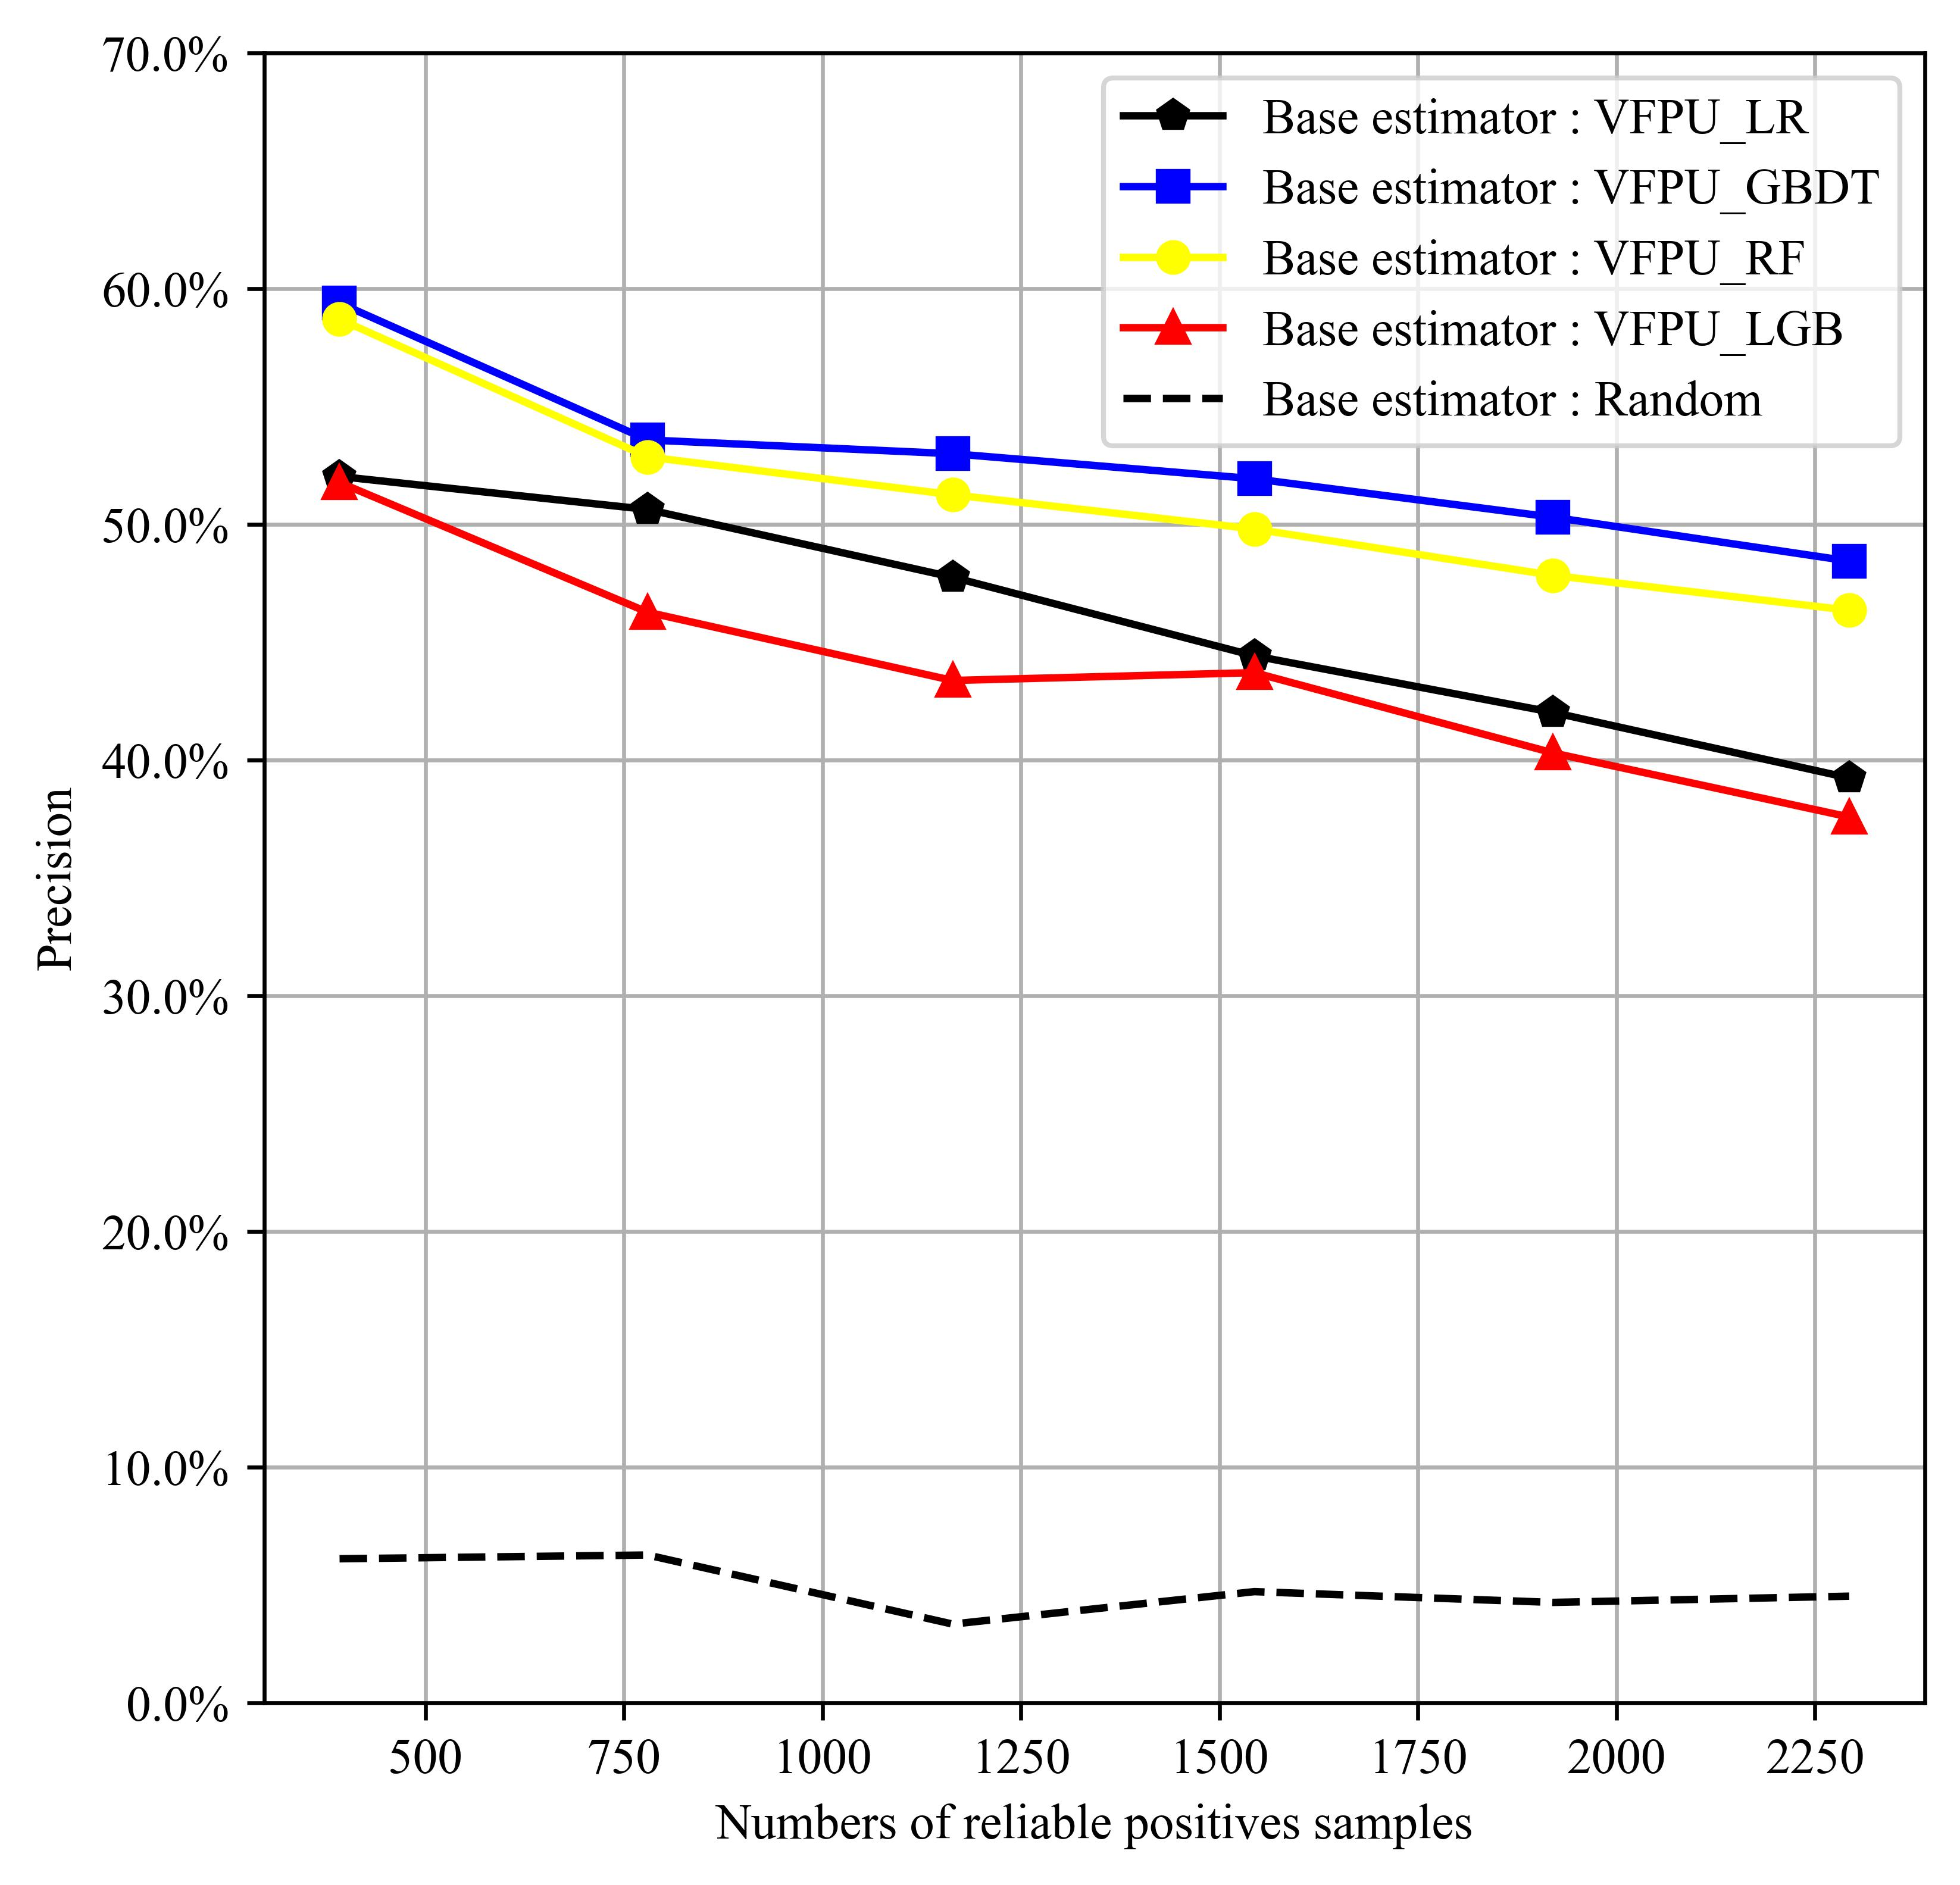
\includegraphics[width=0.9\textwidth,height=5.1cm]{./Figure 2 (1) in JEPG format}
		\caption{Precision}
%		\vspace{0cm}
		\label{RQ2.1.sub1}
	\end{subfigure}
%	\hfill
%    \hspace{-1cm}
	\begin{subfigure}{0.45\textwidth}
		\centering
		\captionsetup{skip=4pt}
		\captionsetup{size=scriptsize}
		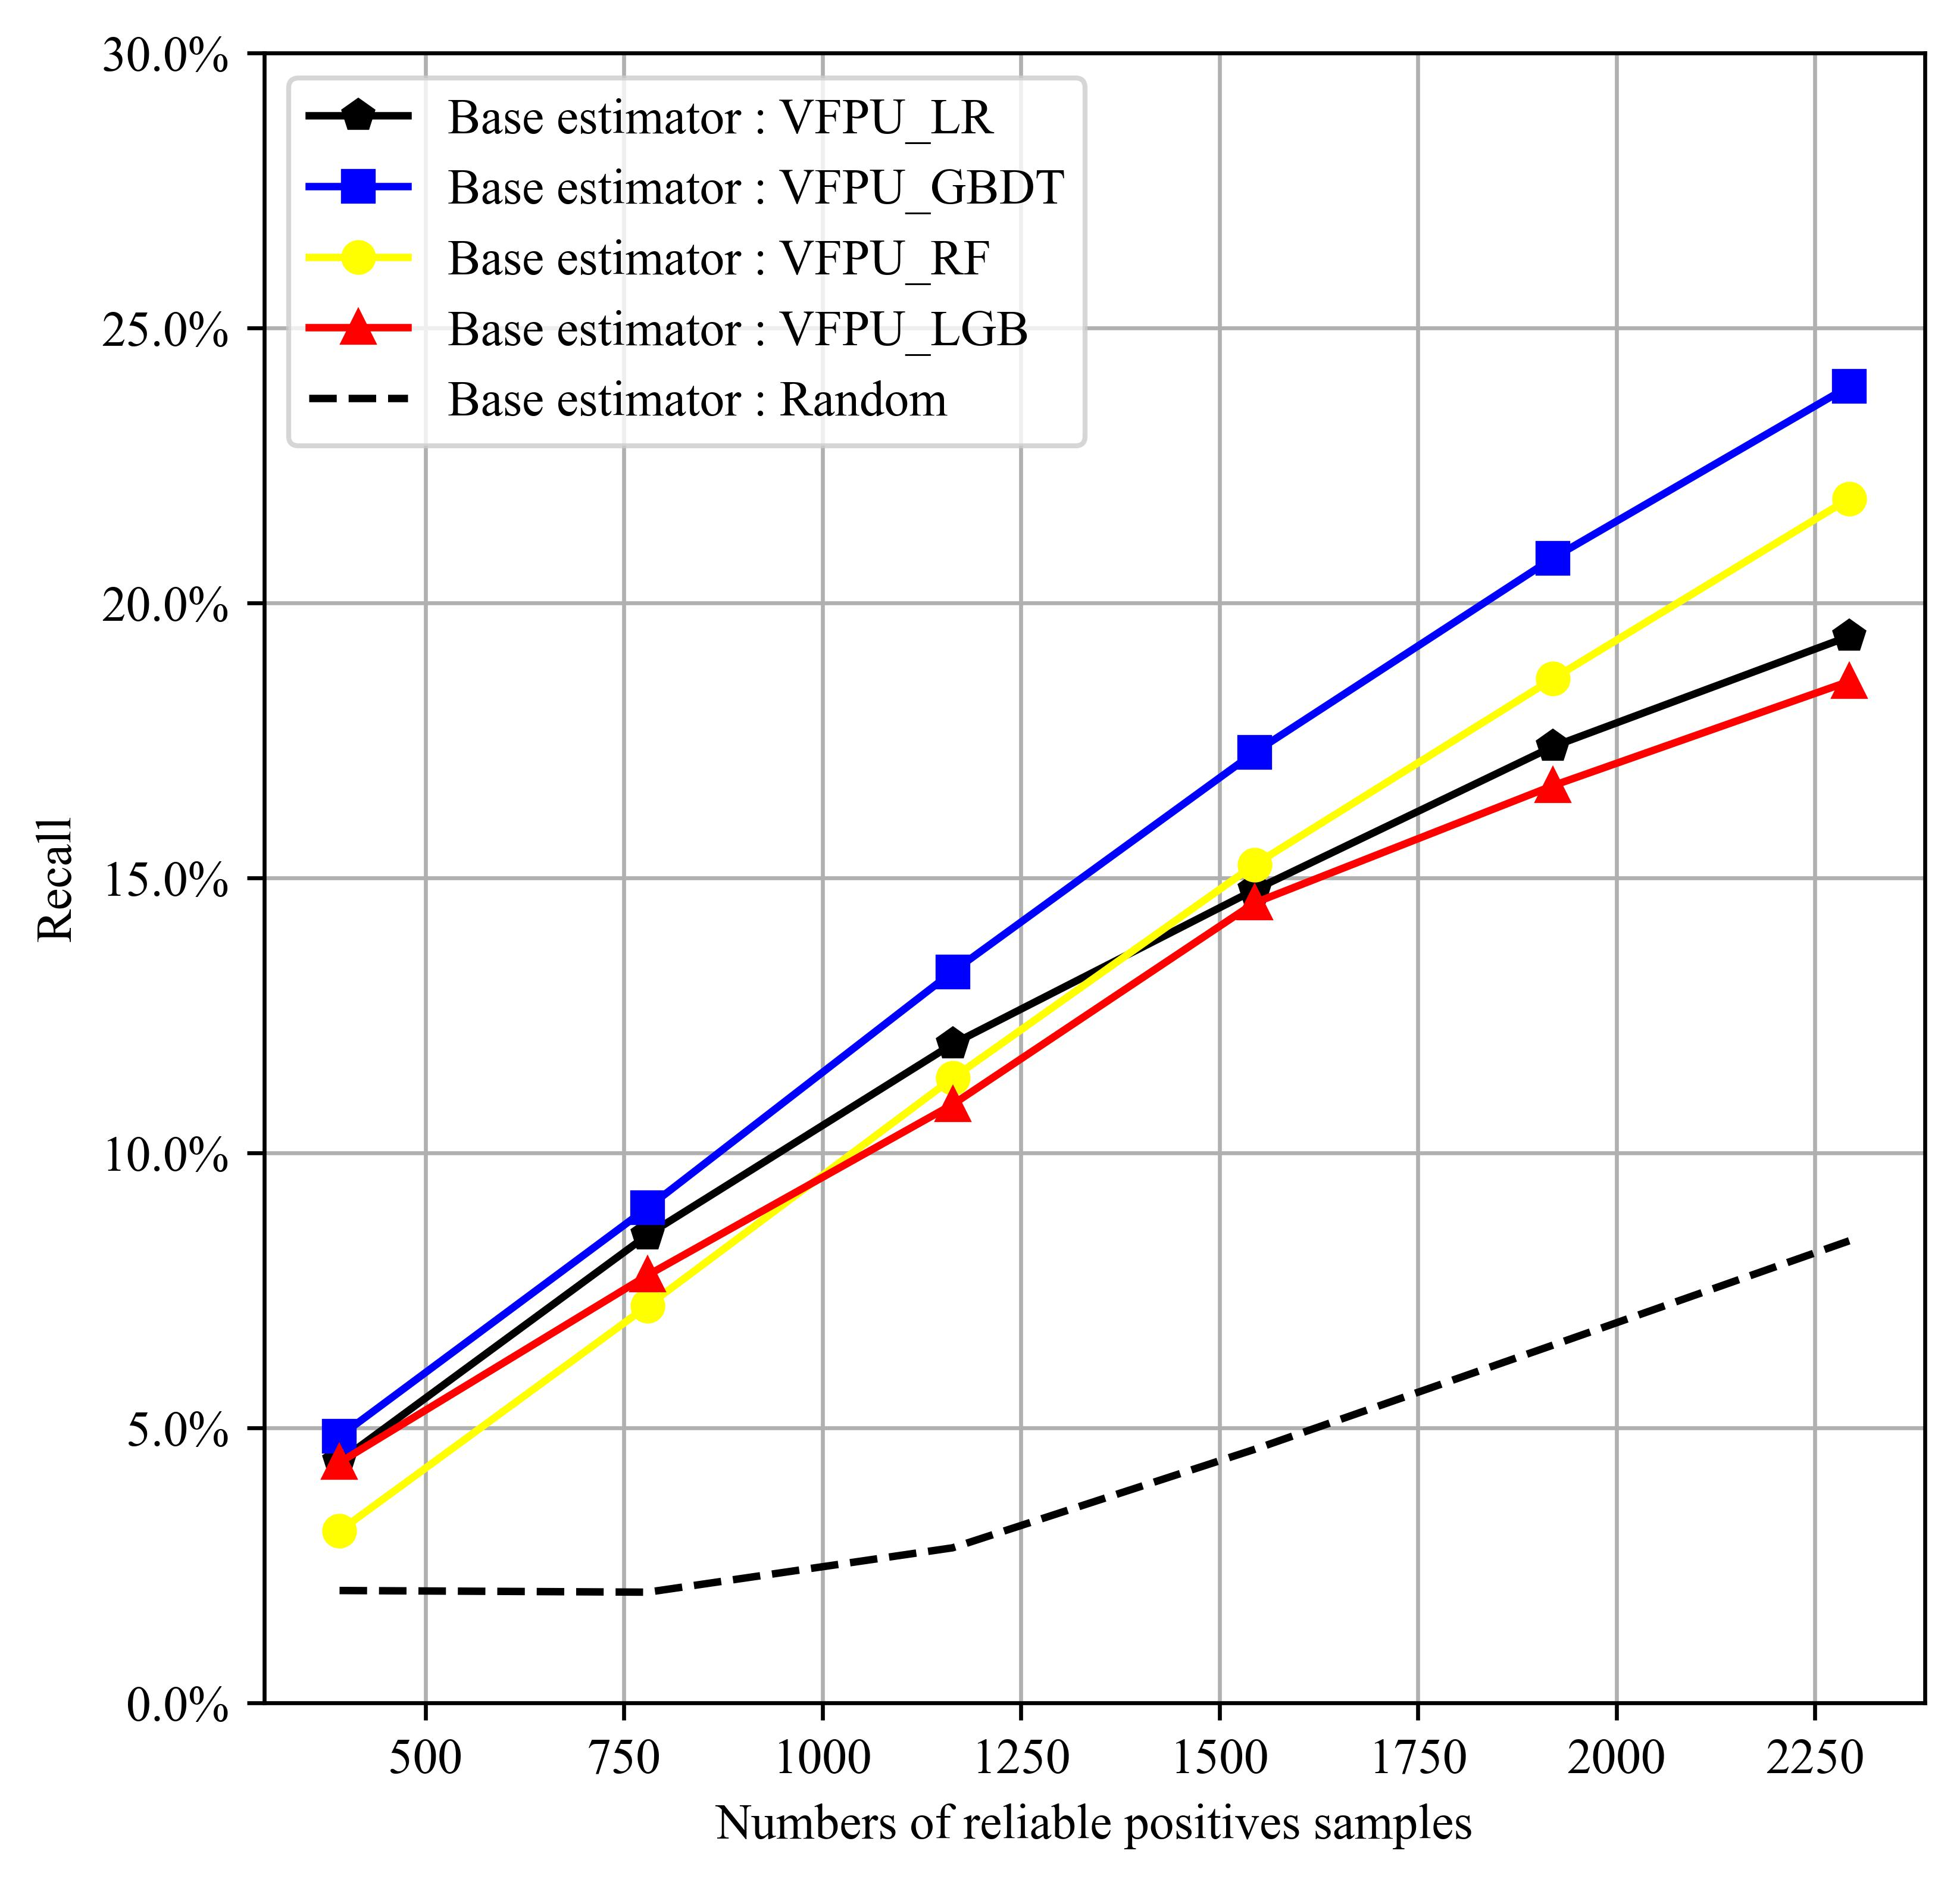
\includegraphics[width=0.9\textwidth,height=5.1cm]{./Figure 2 (2) in JEPG format}
		\caption{Recall}
		\label{RQ2.1.sub2}
	\end{subfigure}
	
%	\vspace{0.05cm}
	
	\begin{subfigure}{0.45\textwidth}
		\centering
		\captionsetup{skip=4pt}
		\captionsetup{size=scriptsize}
		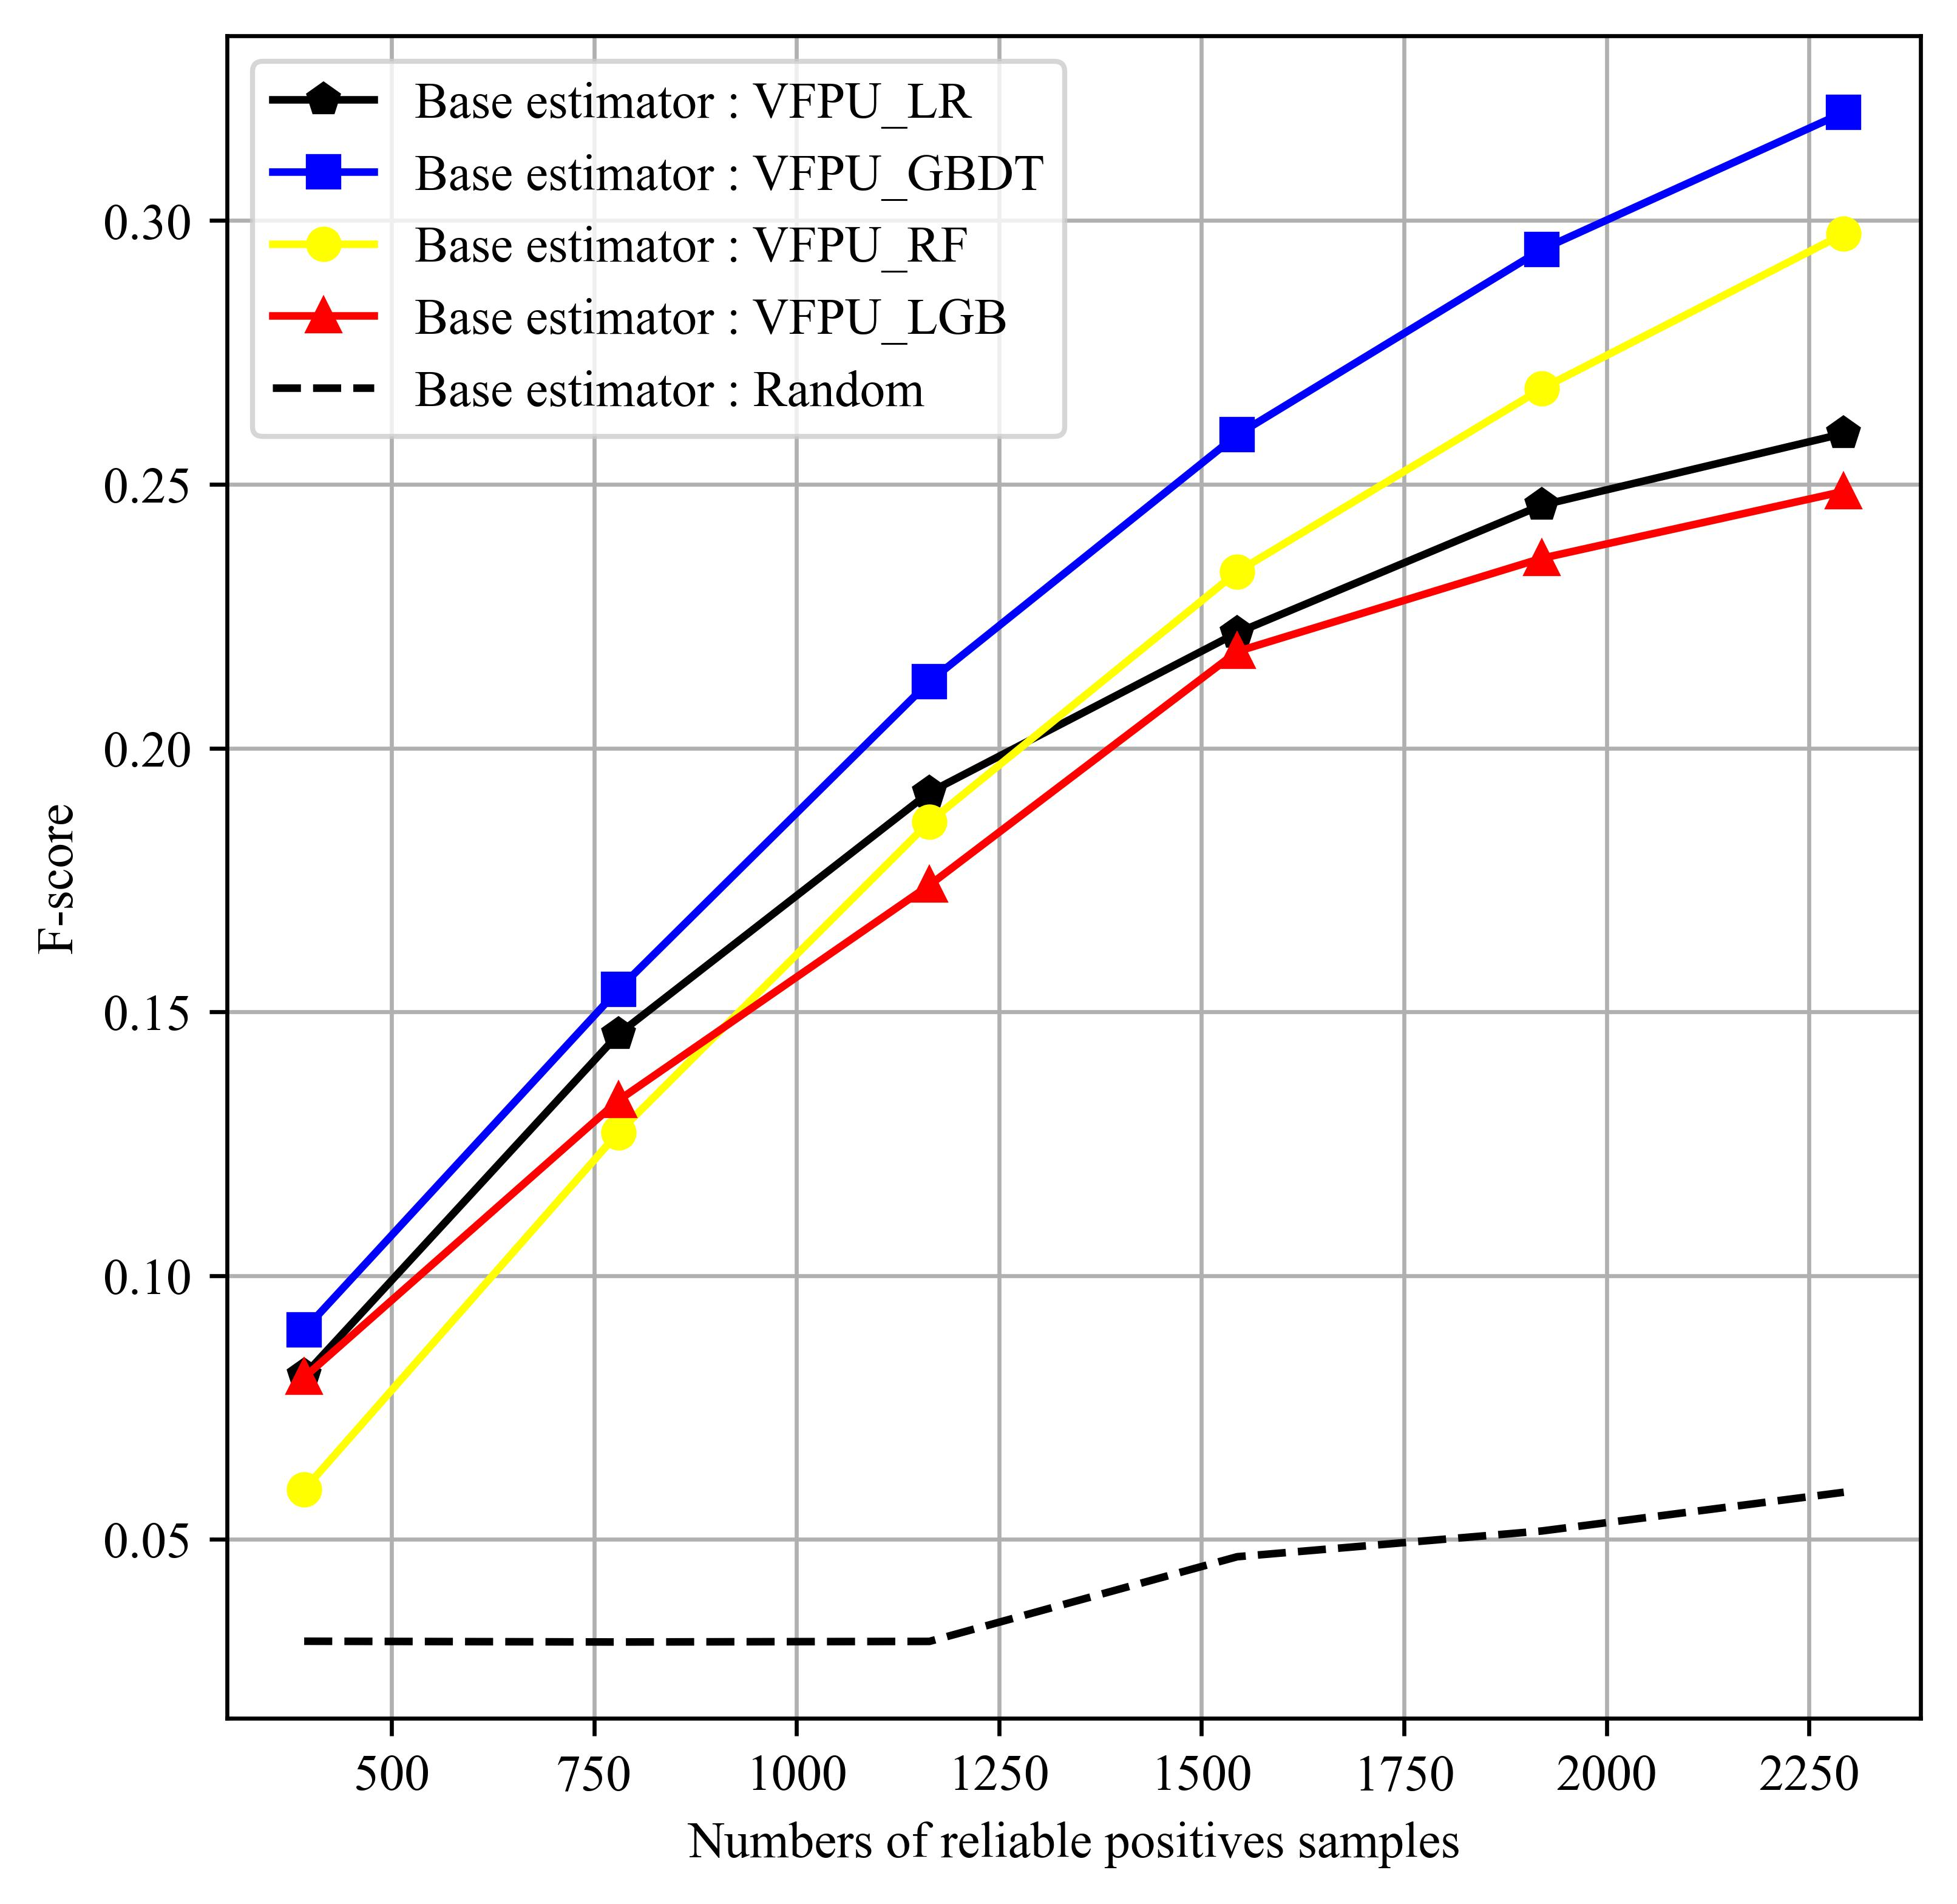
\includegraphics[width=0.9\textwidth,height=5.1cm]{./Figure 2 (3) in JEPG format}
		\caption{F-score}
		\label{RQ2.1.sub3}
	\end{subfigure}
%\hfill
	\begin{subfigure}{0.45\textwidth}
		\centering
		\captionsetup{skip=4pt}
		\captionsetup{size=scriptsize}
		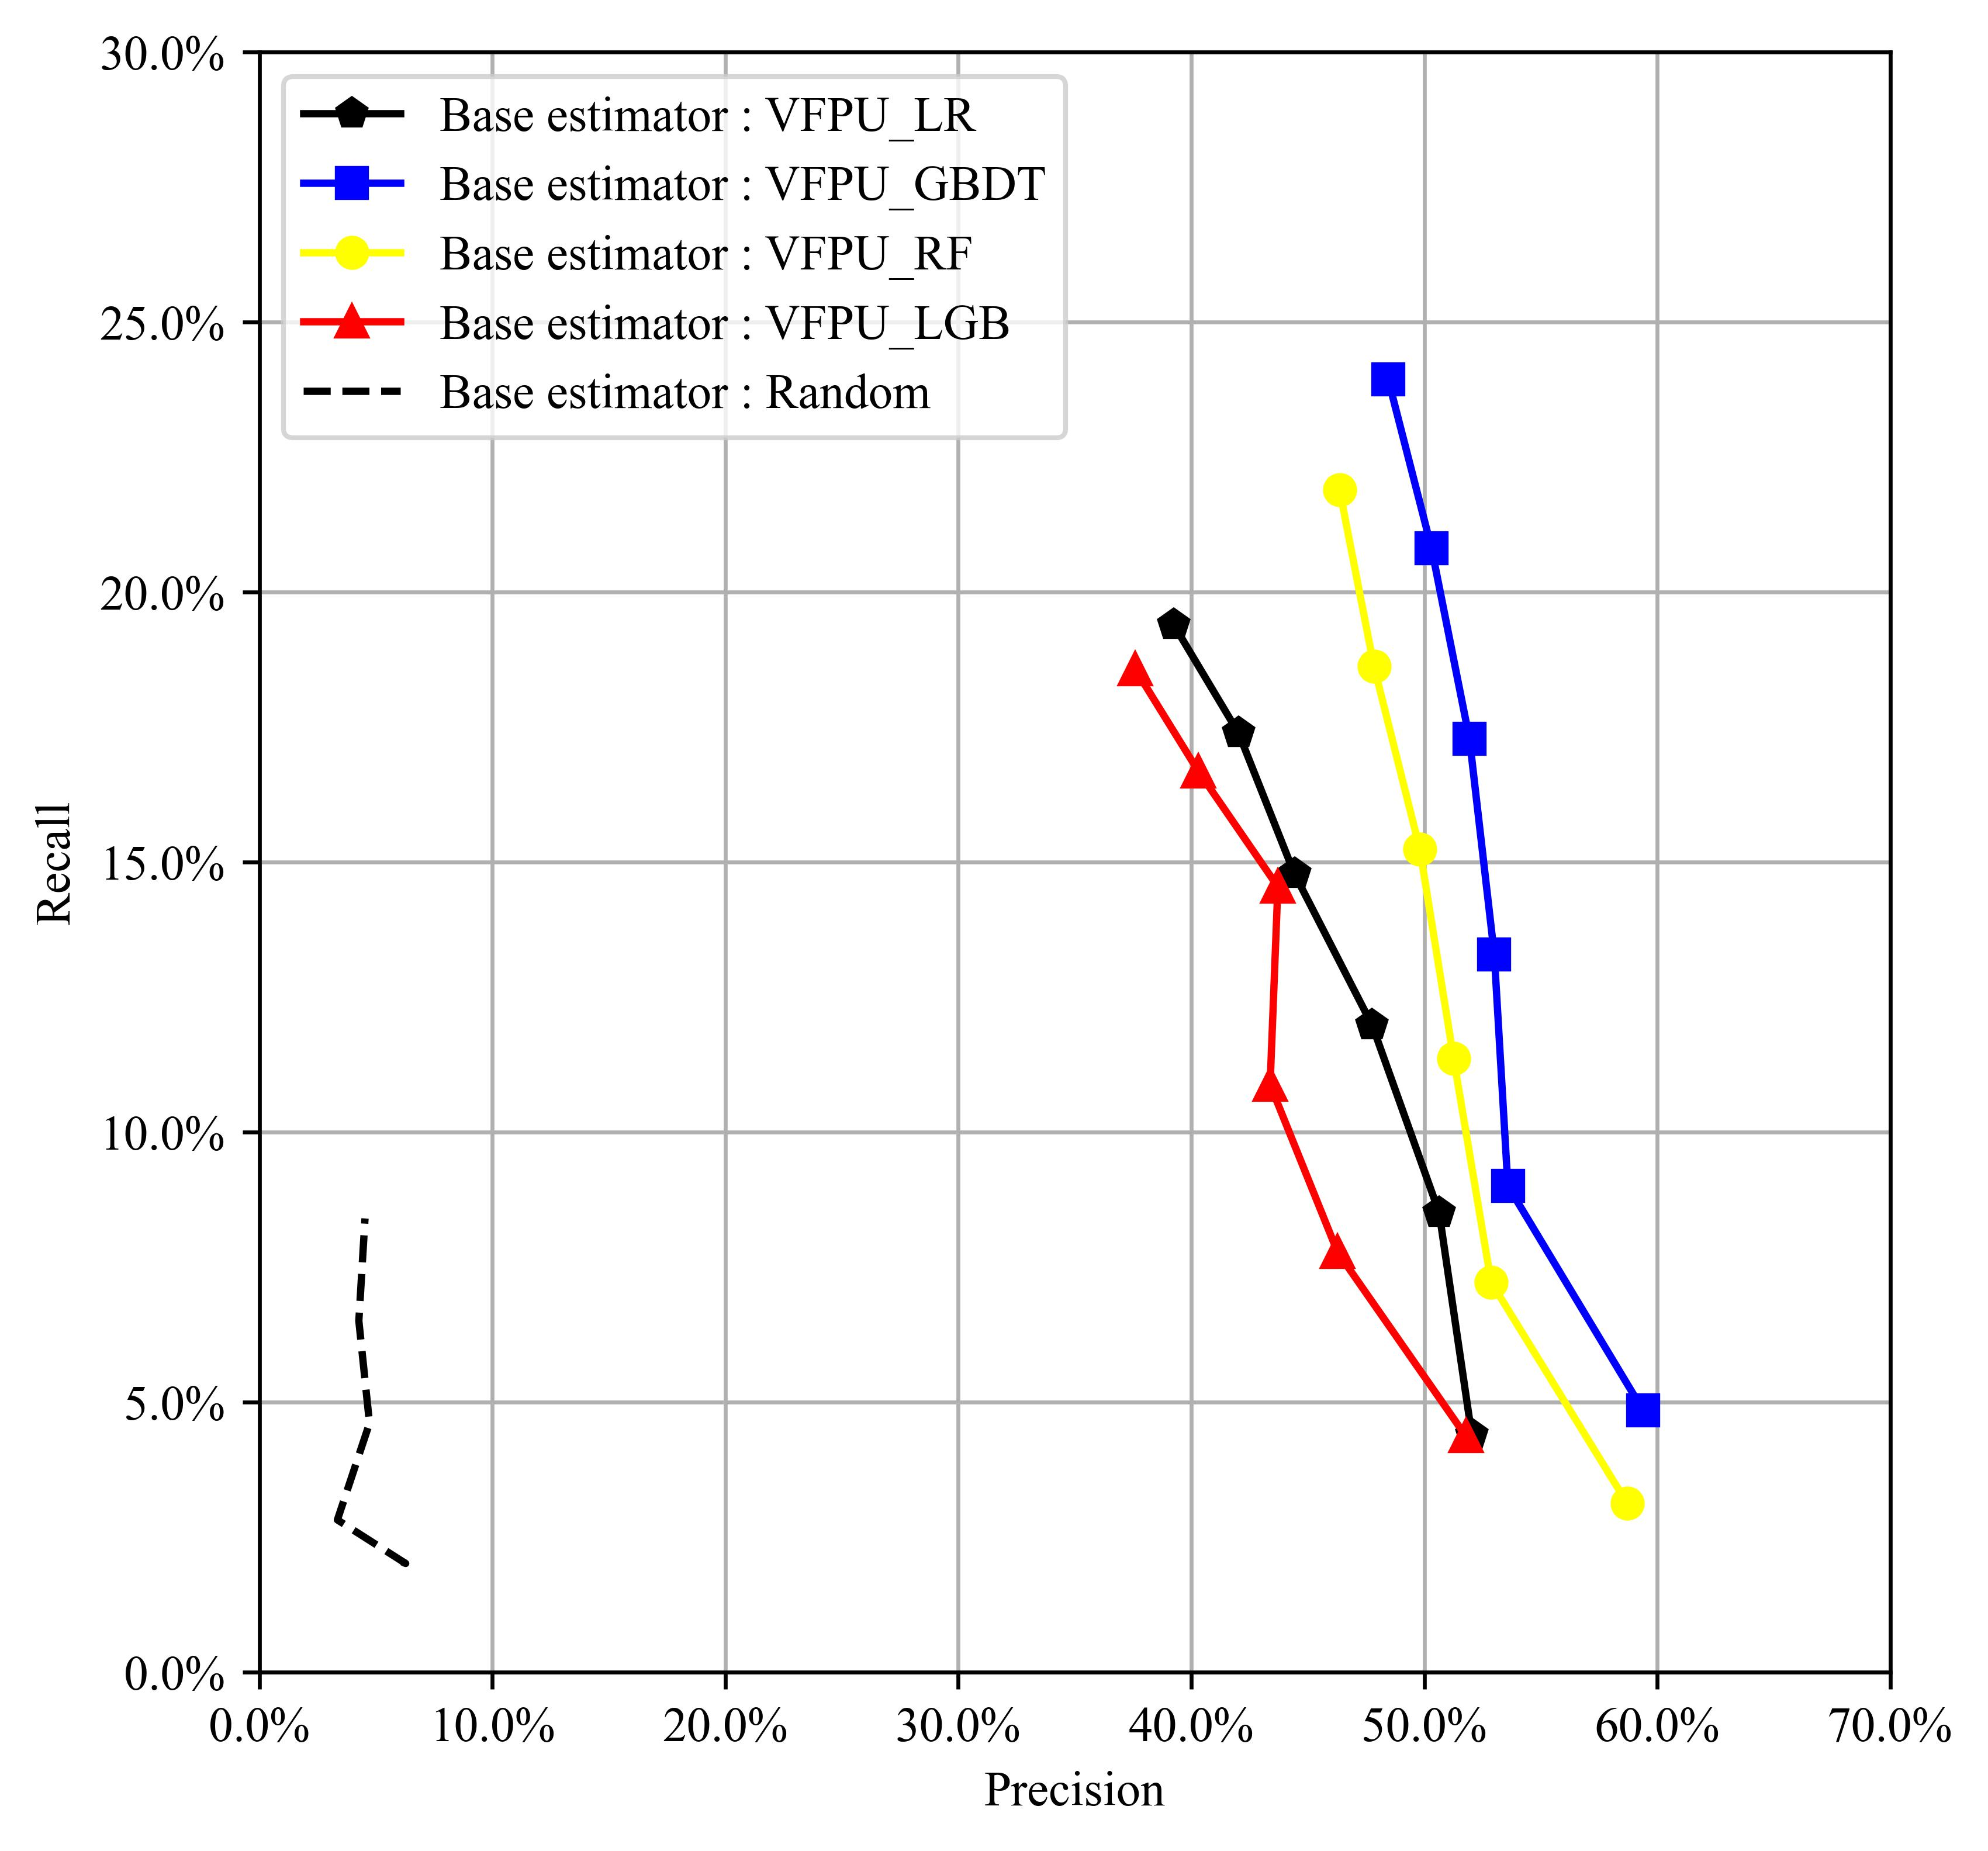
\includegraphics[width=0.95\textwidth,height=5.1cm]{./Figure 2 (4) in JEPG format}
		\caption{Precision-Recall}
		\label{RQ2.1.sub4}
	\end{subfigure}
	
	\caption{Performance of Different Base Estimators with Varying Reliable Positive Samples: (1) Precision; (2) Recall; (3) F-score; (4) Precision-Recall (The Bank Marketing Dataset)}
	\label{RQ2.1}
\end{figure*}


\begin{figure*}[!htbp]
	\centering
	\captionsetup{size=footnotesize}
	\begin{subfigure}{0.45\textwidth}
		\centering
		\captionsetup{skip=4pt}
		\captionsetup{size=scriptsize}
		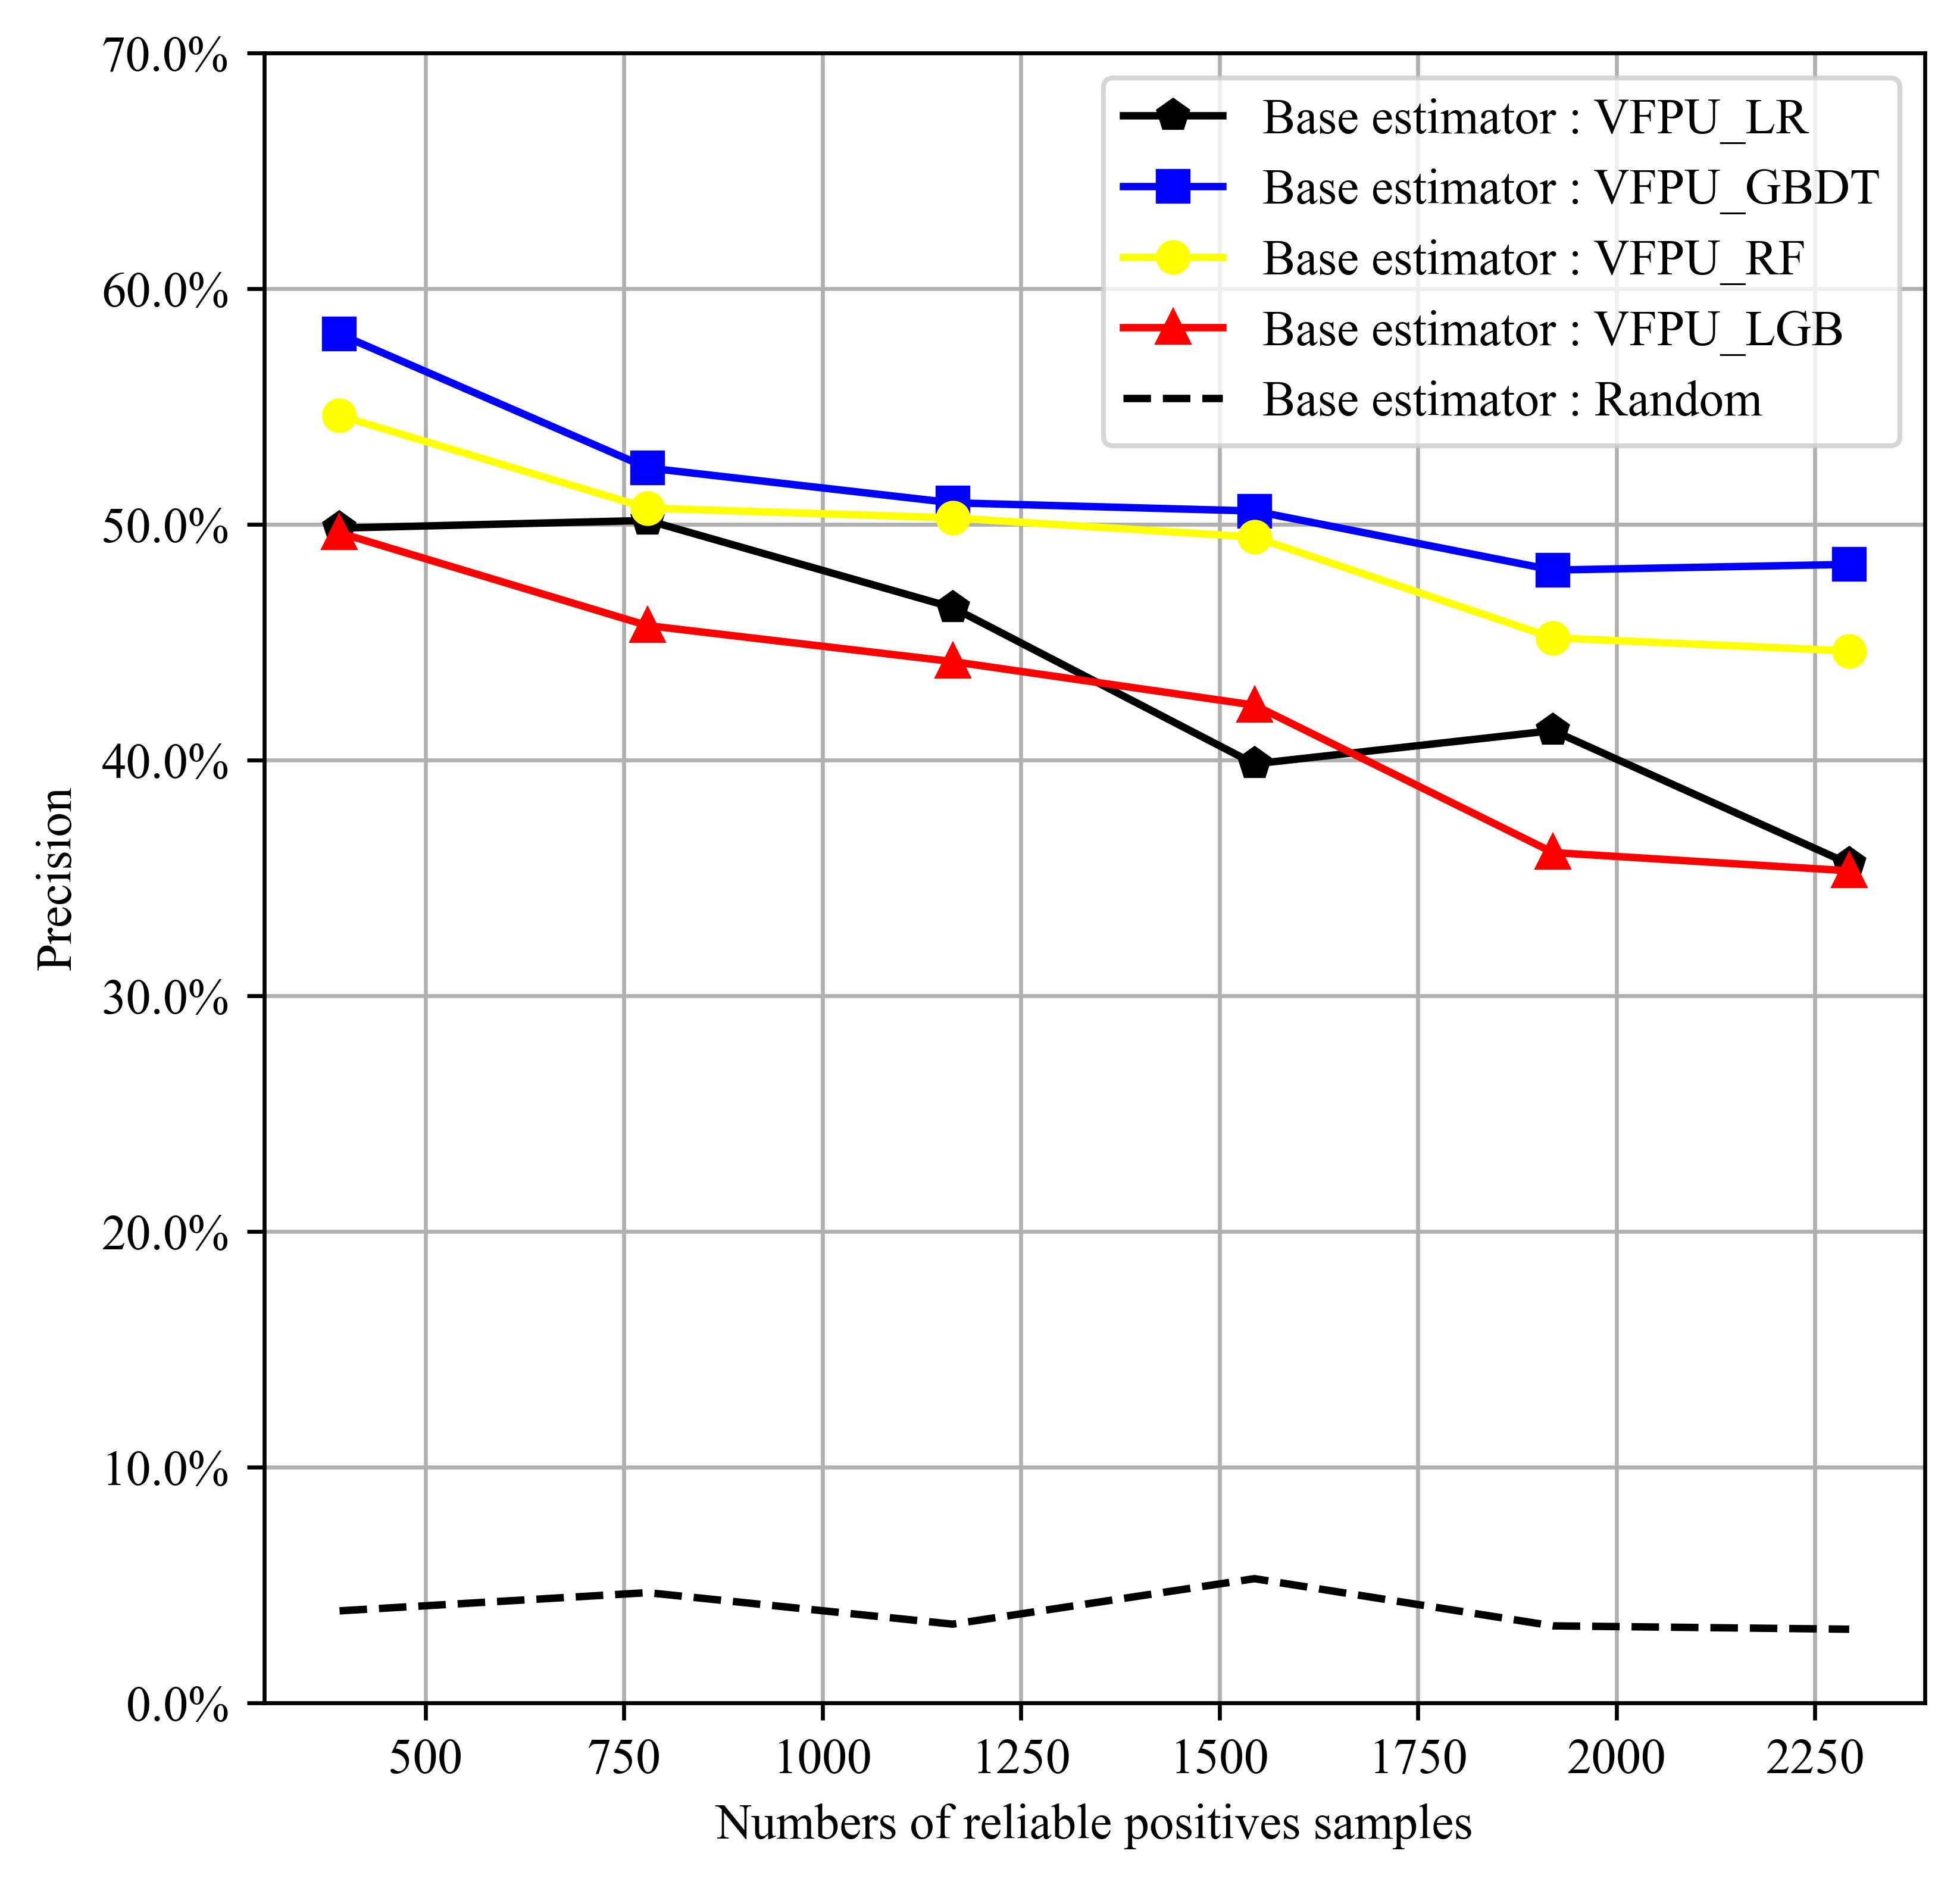
\includegraphics[width=0.9\textwidth,height=5.1cm]{./Figure 3 (1) in JEPG format}
		\caption{Precision}
		\label{RQ2.2.sub1}
	\end{subfigure}
%\hfill
	\begin{subfigure}{0.45\textwidth}
		\centering
		\captionsetup{skip=4pt}
		\captionsetup{size=scriptsize}
		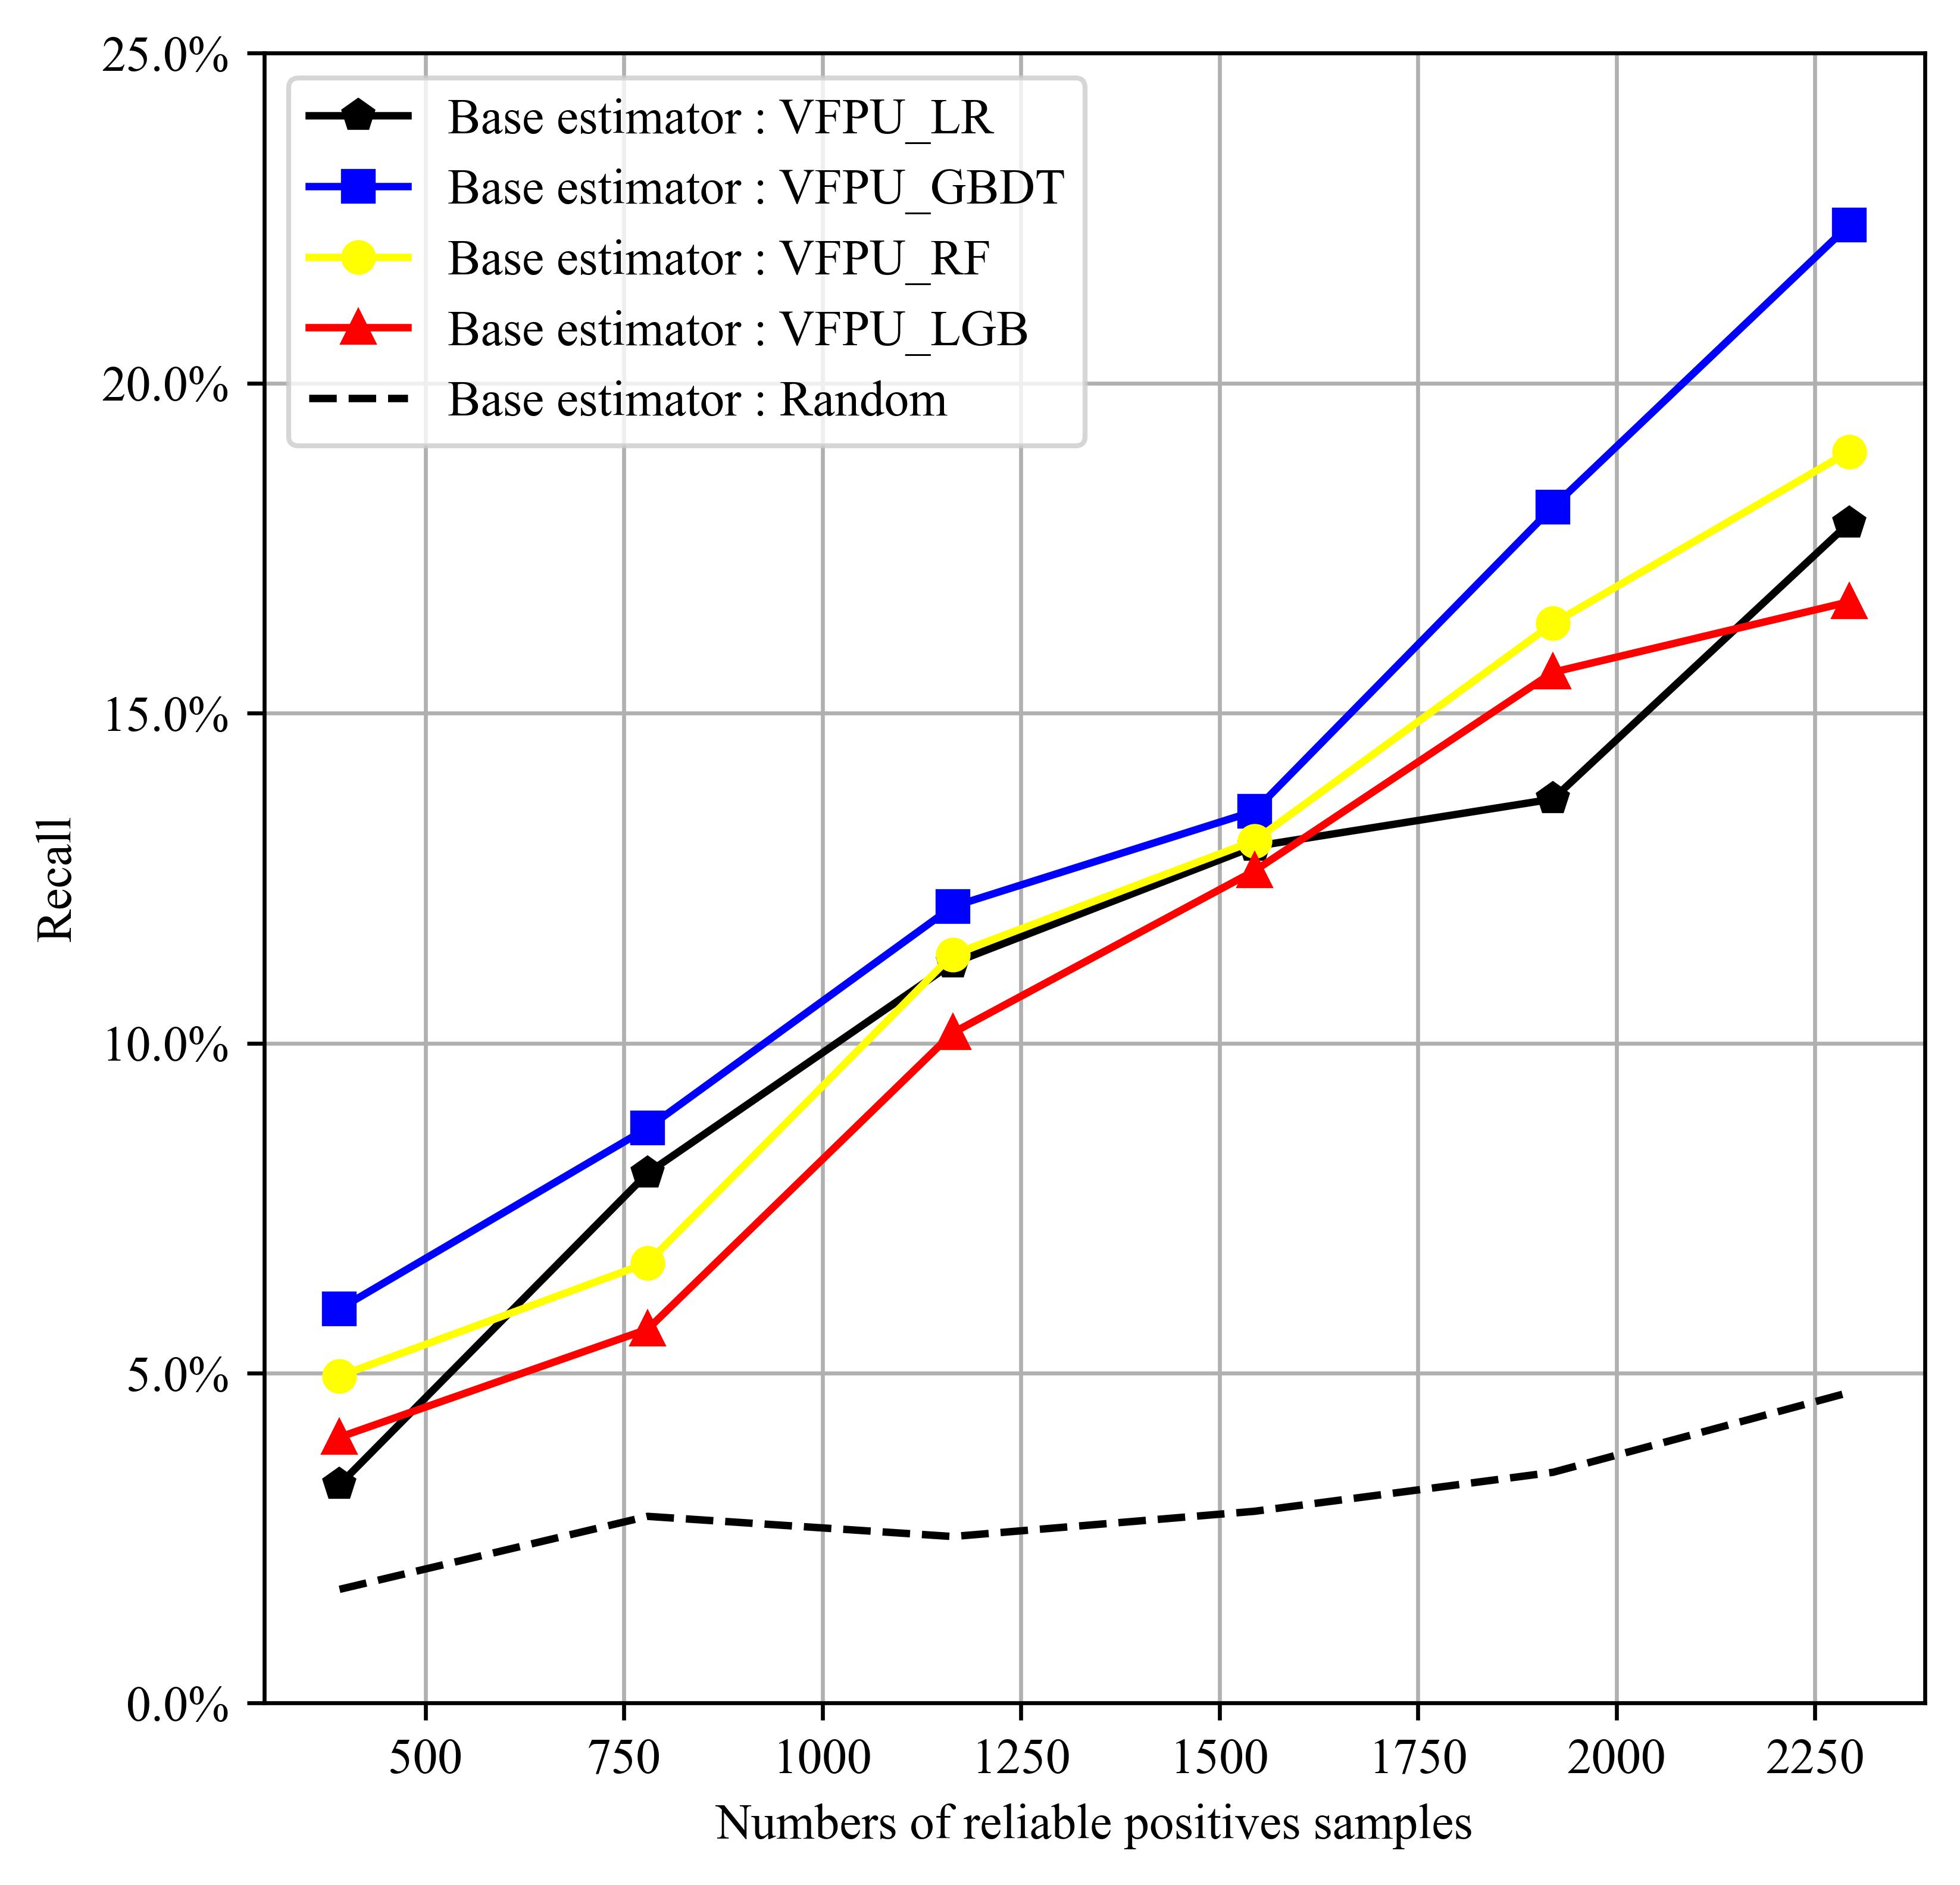
\includegraphics[width=0.9\textwidth,height=5.1cm]{./Figure 3 (2) in JEPG format}
		\caption{Recall}
		\label{RQ2.2.sub2}
	\end{subfigure}
	
%	\vspace{0.05cm}
	
	\begin{subfigure}{0.45\textwidth}
		\centering
		\captionsetup{skip=4pt}
		\captionsetup{size=scriptsize}
		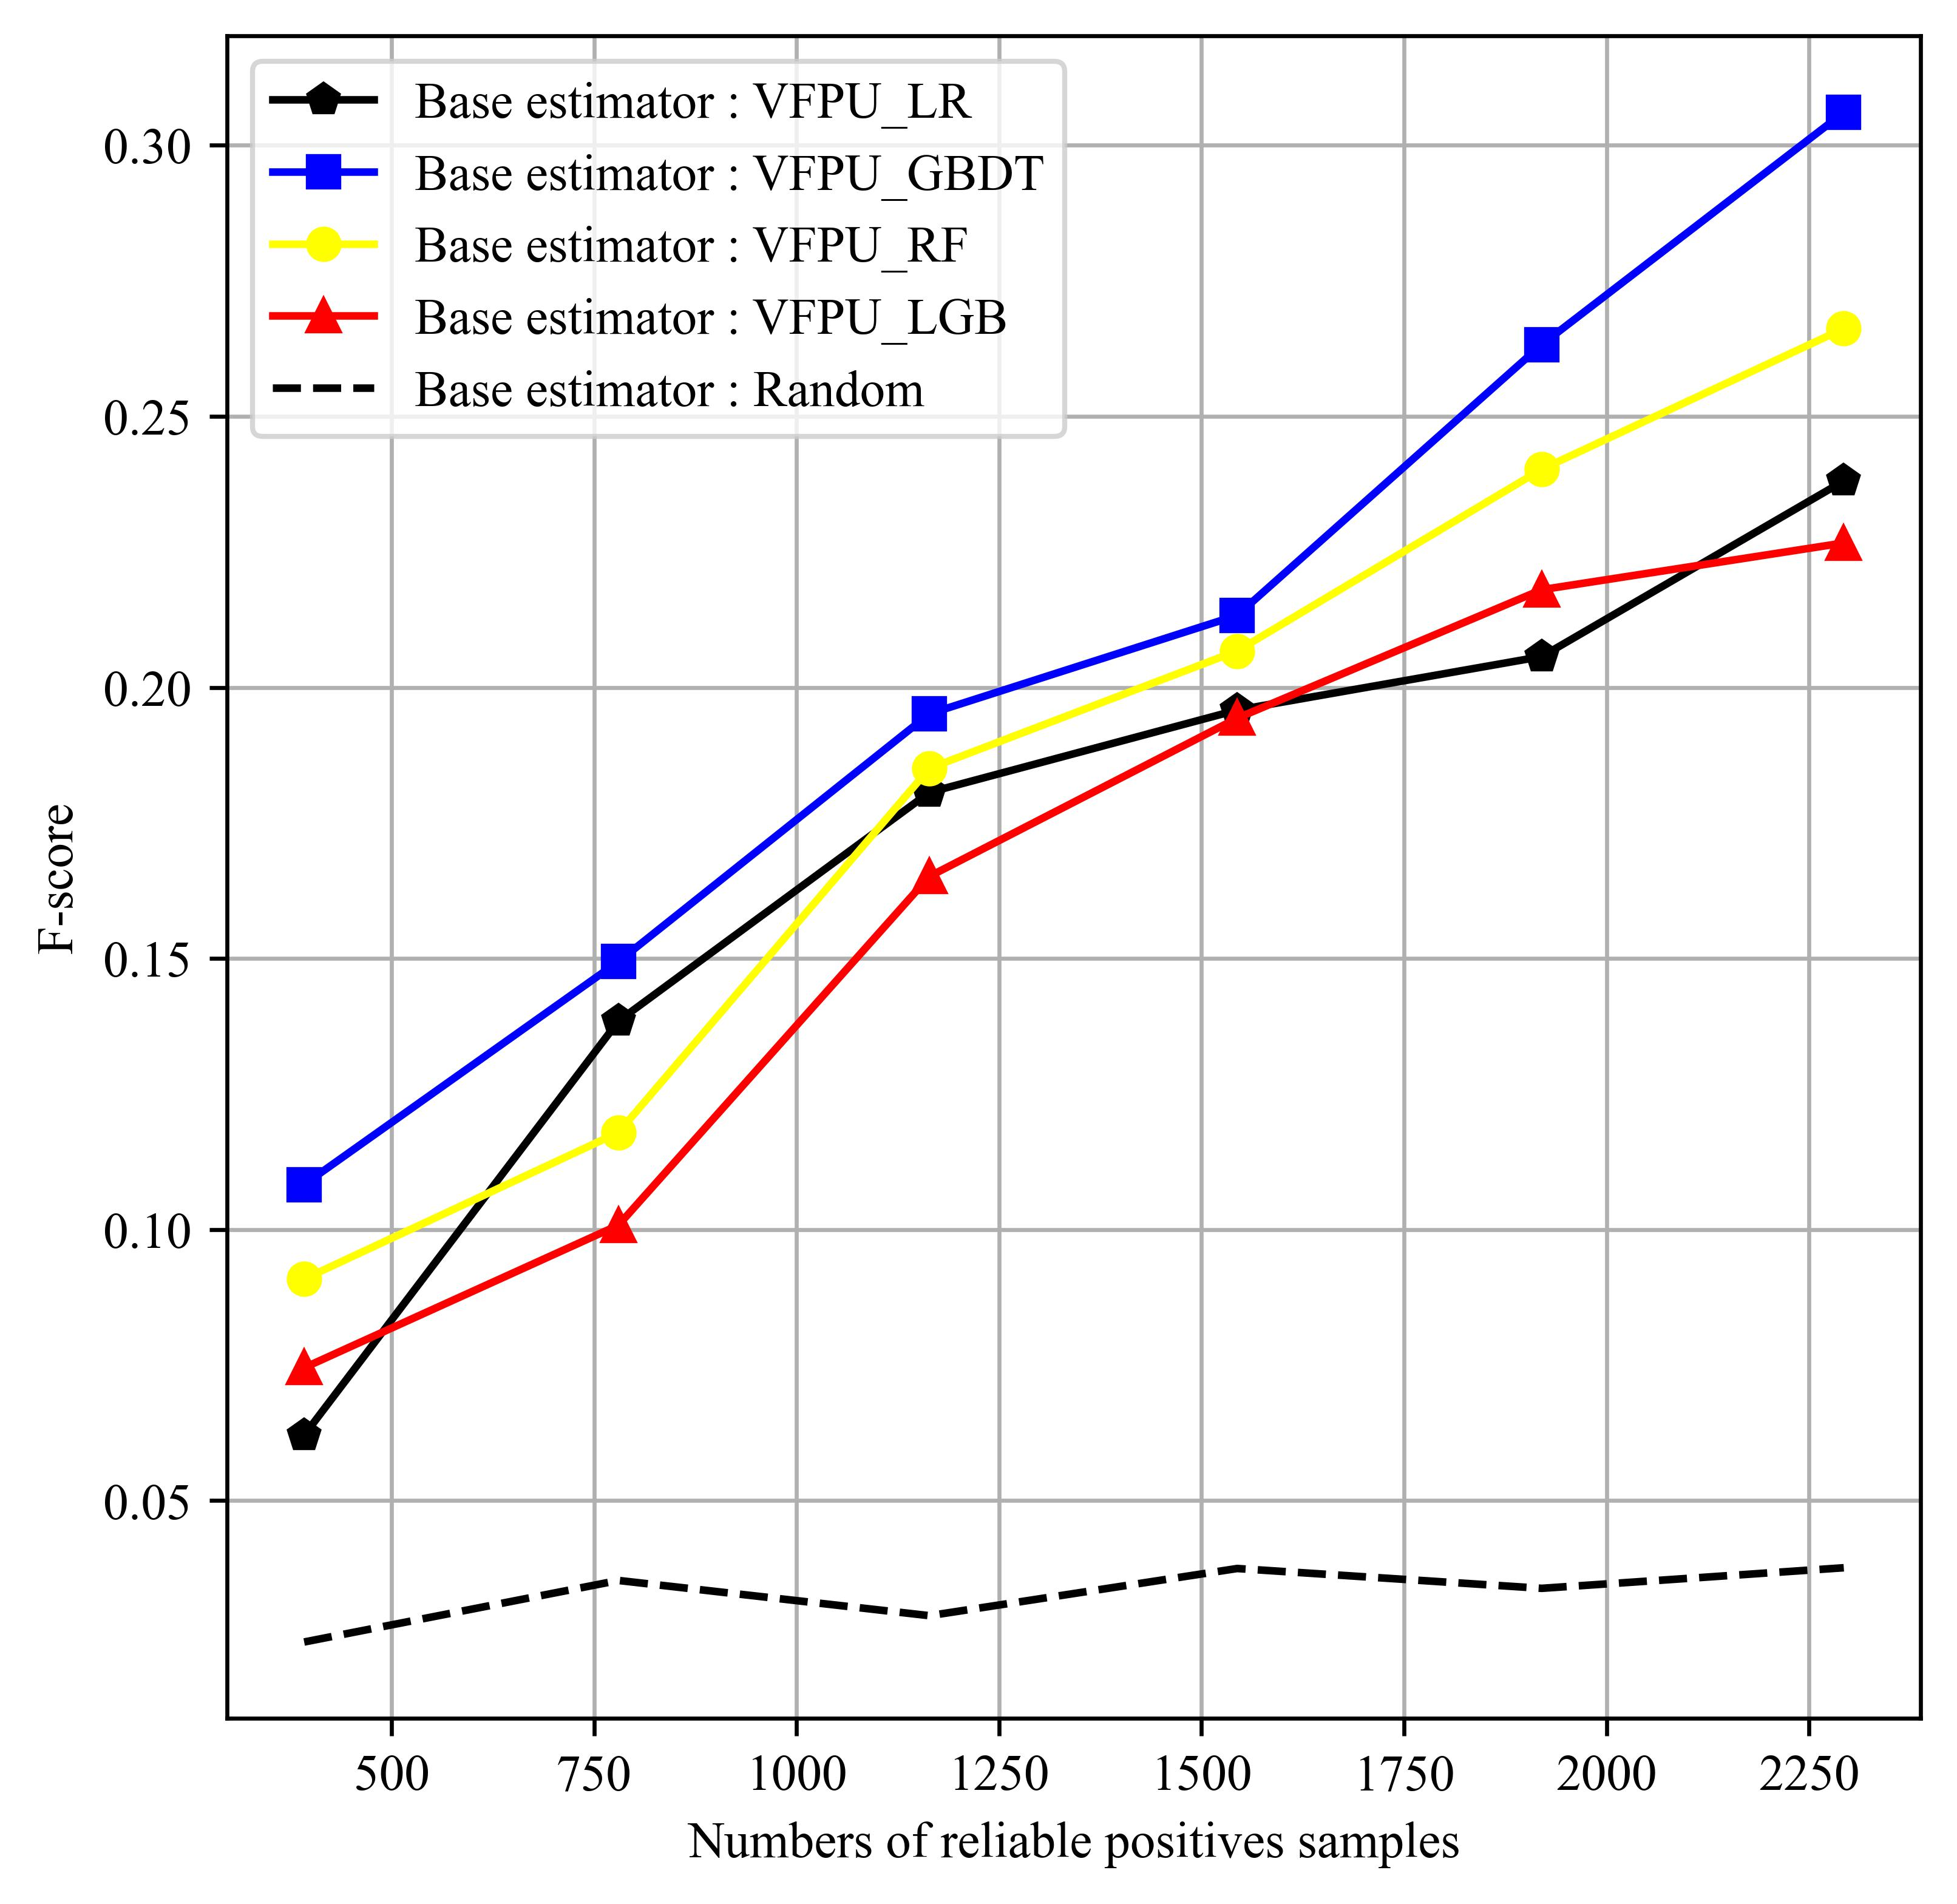
\includegraphics[width=0.9\textwidth,height=5.1cm]{./Figure 3 (3) in JEPG format}
		\caption{F-score}
		\label{RQ2.2.sub3}
	\end{subfigure}
%\hfill
	\begin{subfigure}{0.45\textwidth}
		\centering
		\captionsetup{skip=4pt}
		\captionsetup{size=scriptsize}
		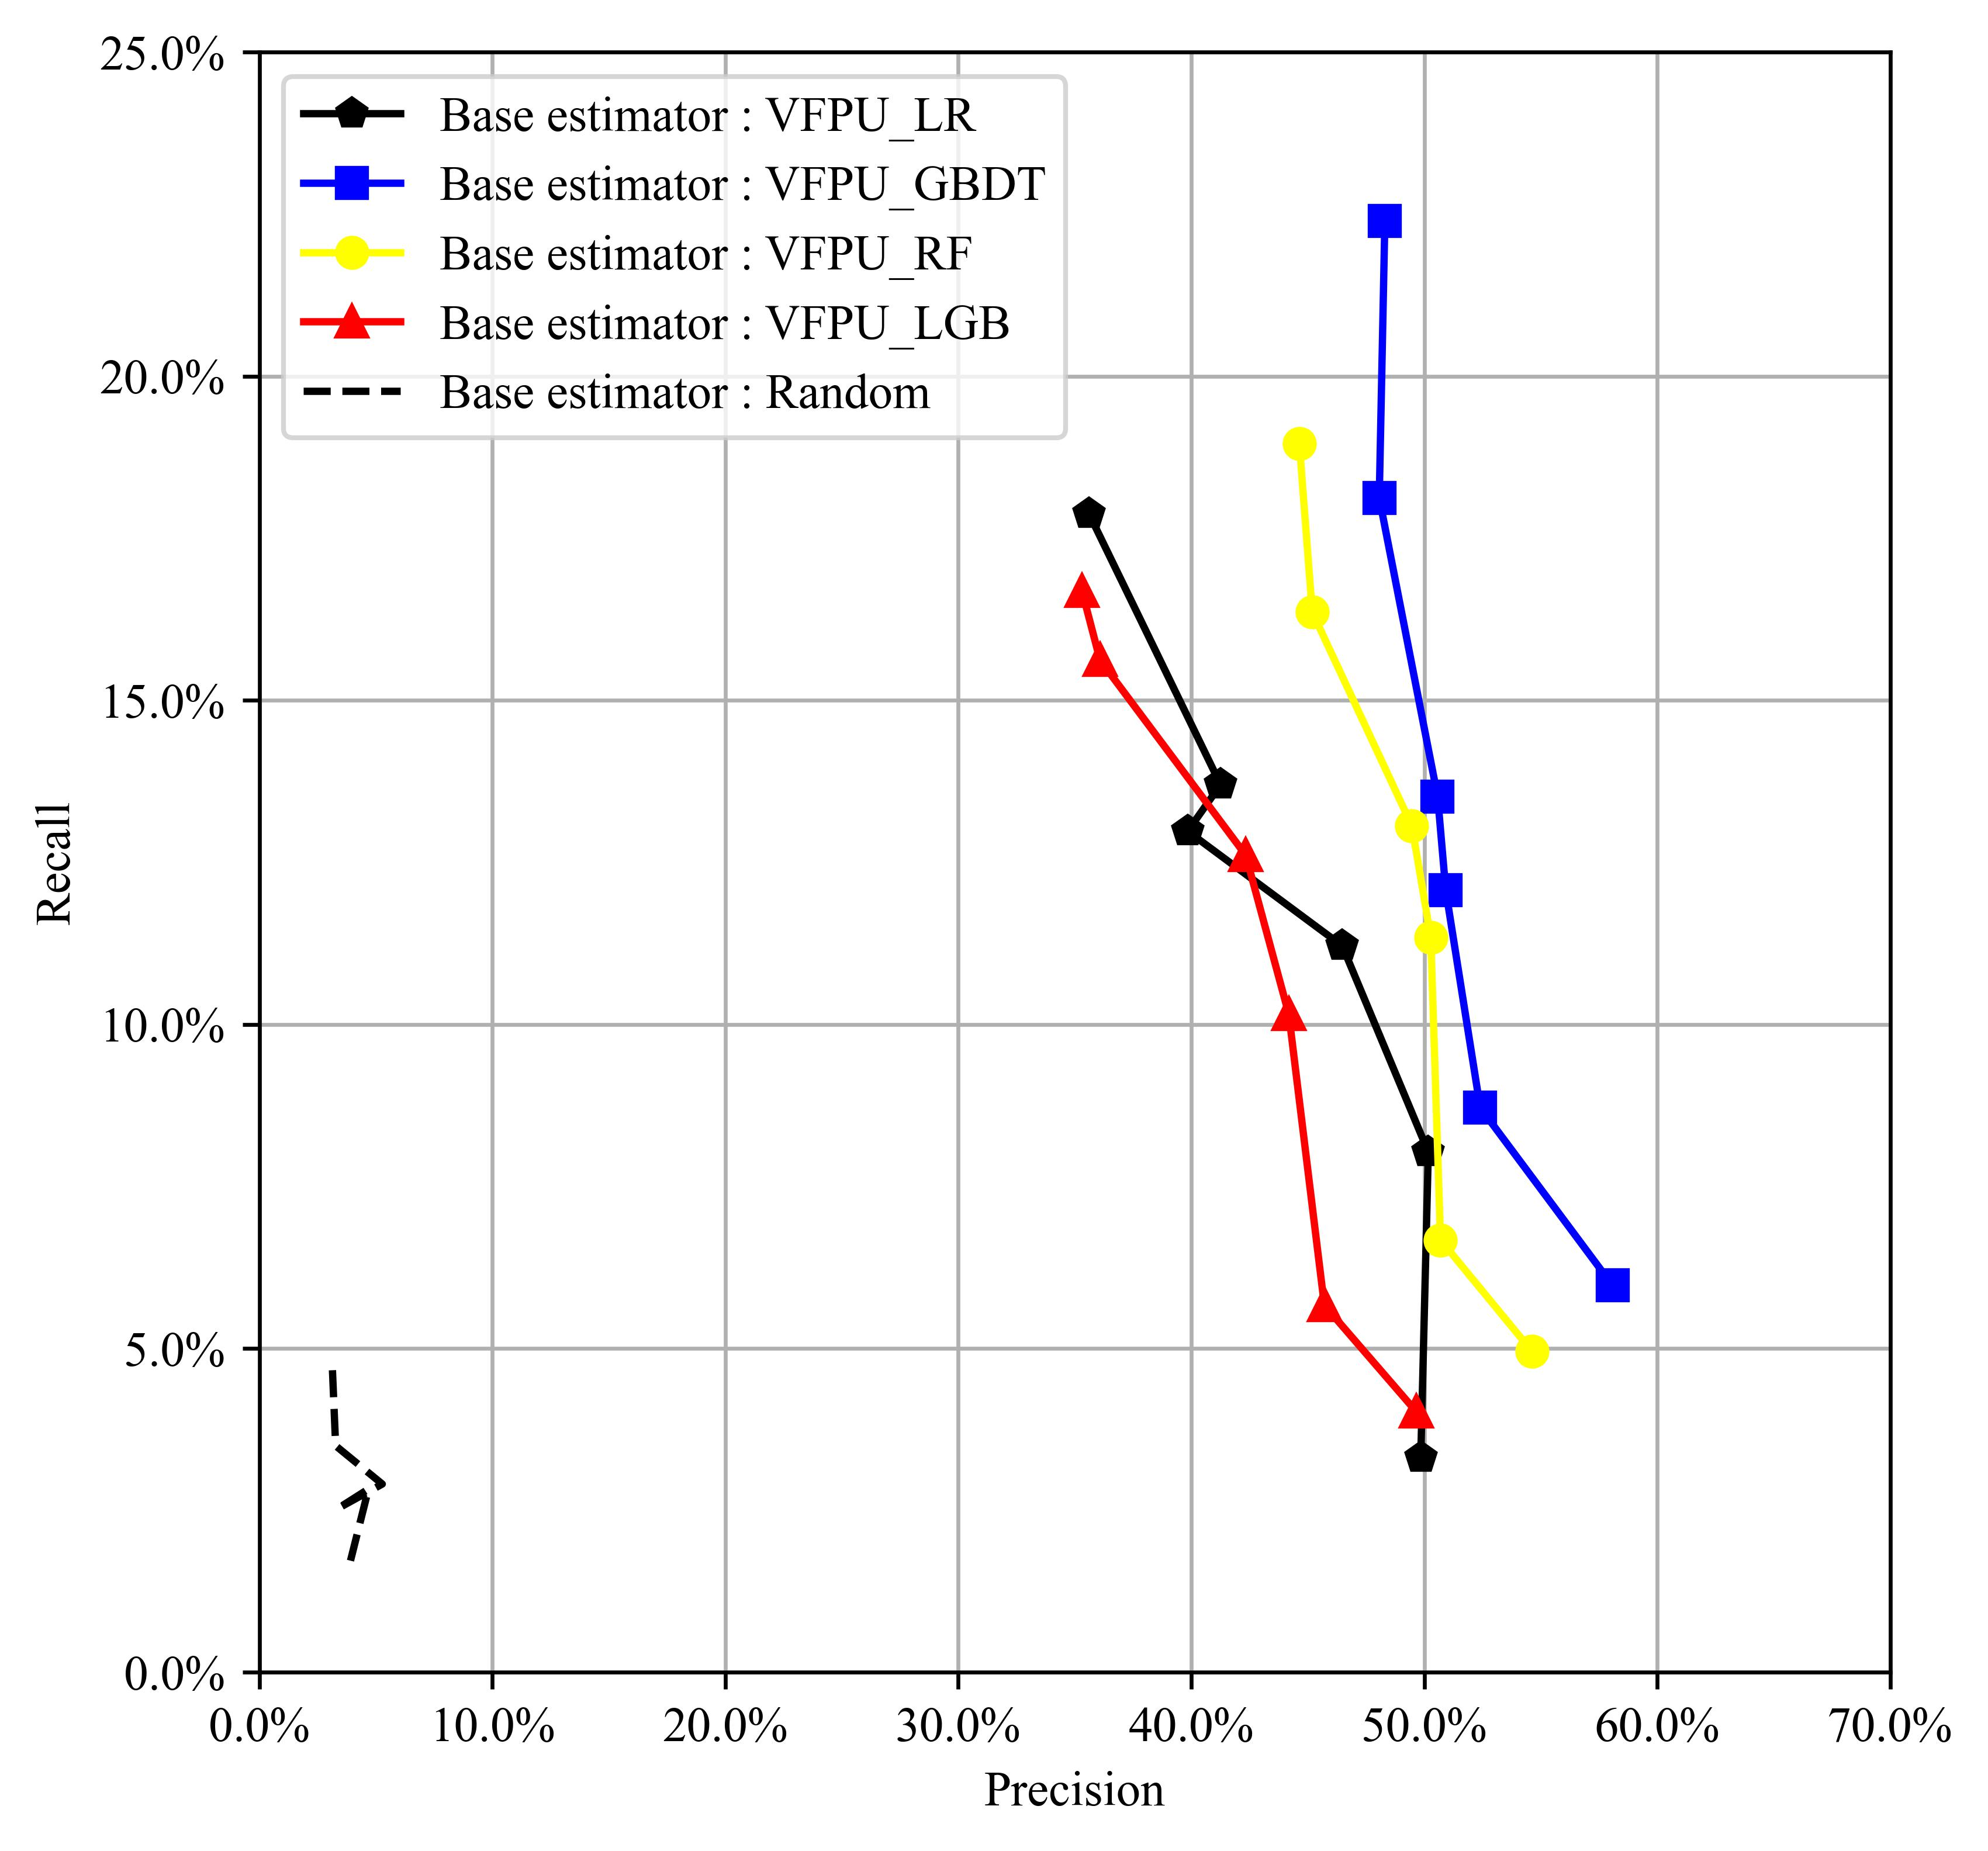
\includegraphics[width=0.9\textwidth,height=5.1cm]{./Figure 3 (4) in JEPG format}
		\caption{Precision-Recall}
		\label{RQ2.2.sub4}
	\end{subfigure}
	
	\caption{Performance of Different Base Estimators with Varying Reliable Positive Samples: (1) Precision; (2) Recall; (3) F-score; (4) Precision-Recall (The Default of Credit Card Clients Dataset)}
	\label{RQ2.2}
\end{figure*}

\begin{figure*}[!htbp]
	\centering
	\captionsetup{size=footnotesize}
	\begin{subfigure}{0.45\textwidth}
		\centering
		\captionsetup{skip=2pt}
		\captionsetup{size=scriptsize}
		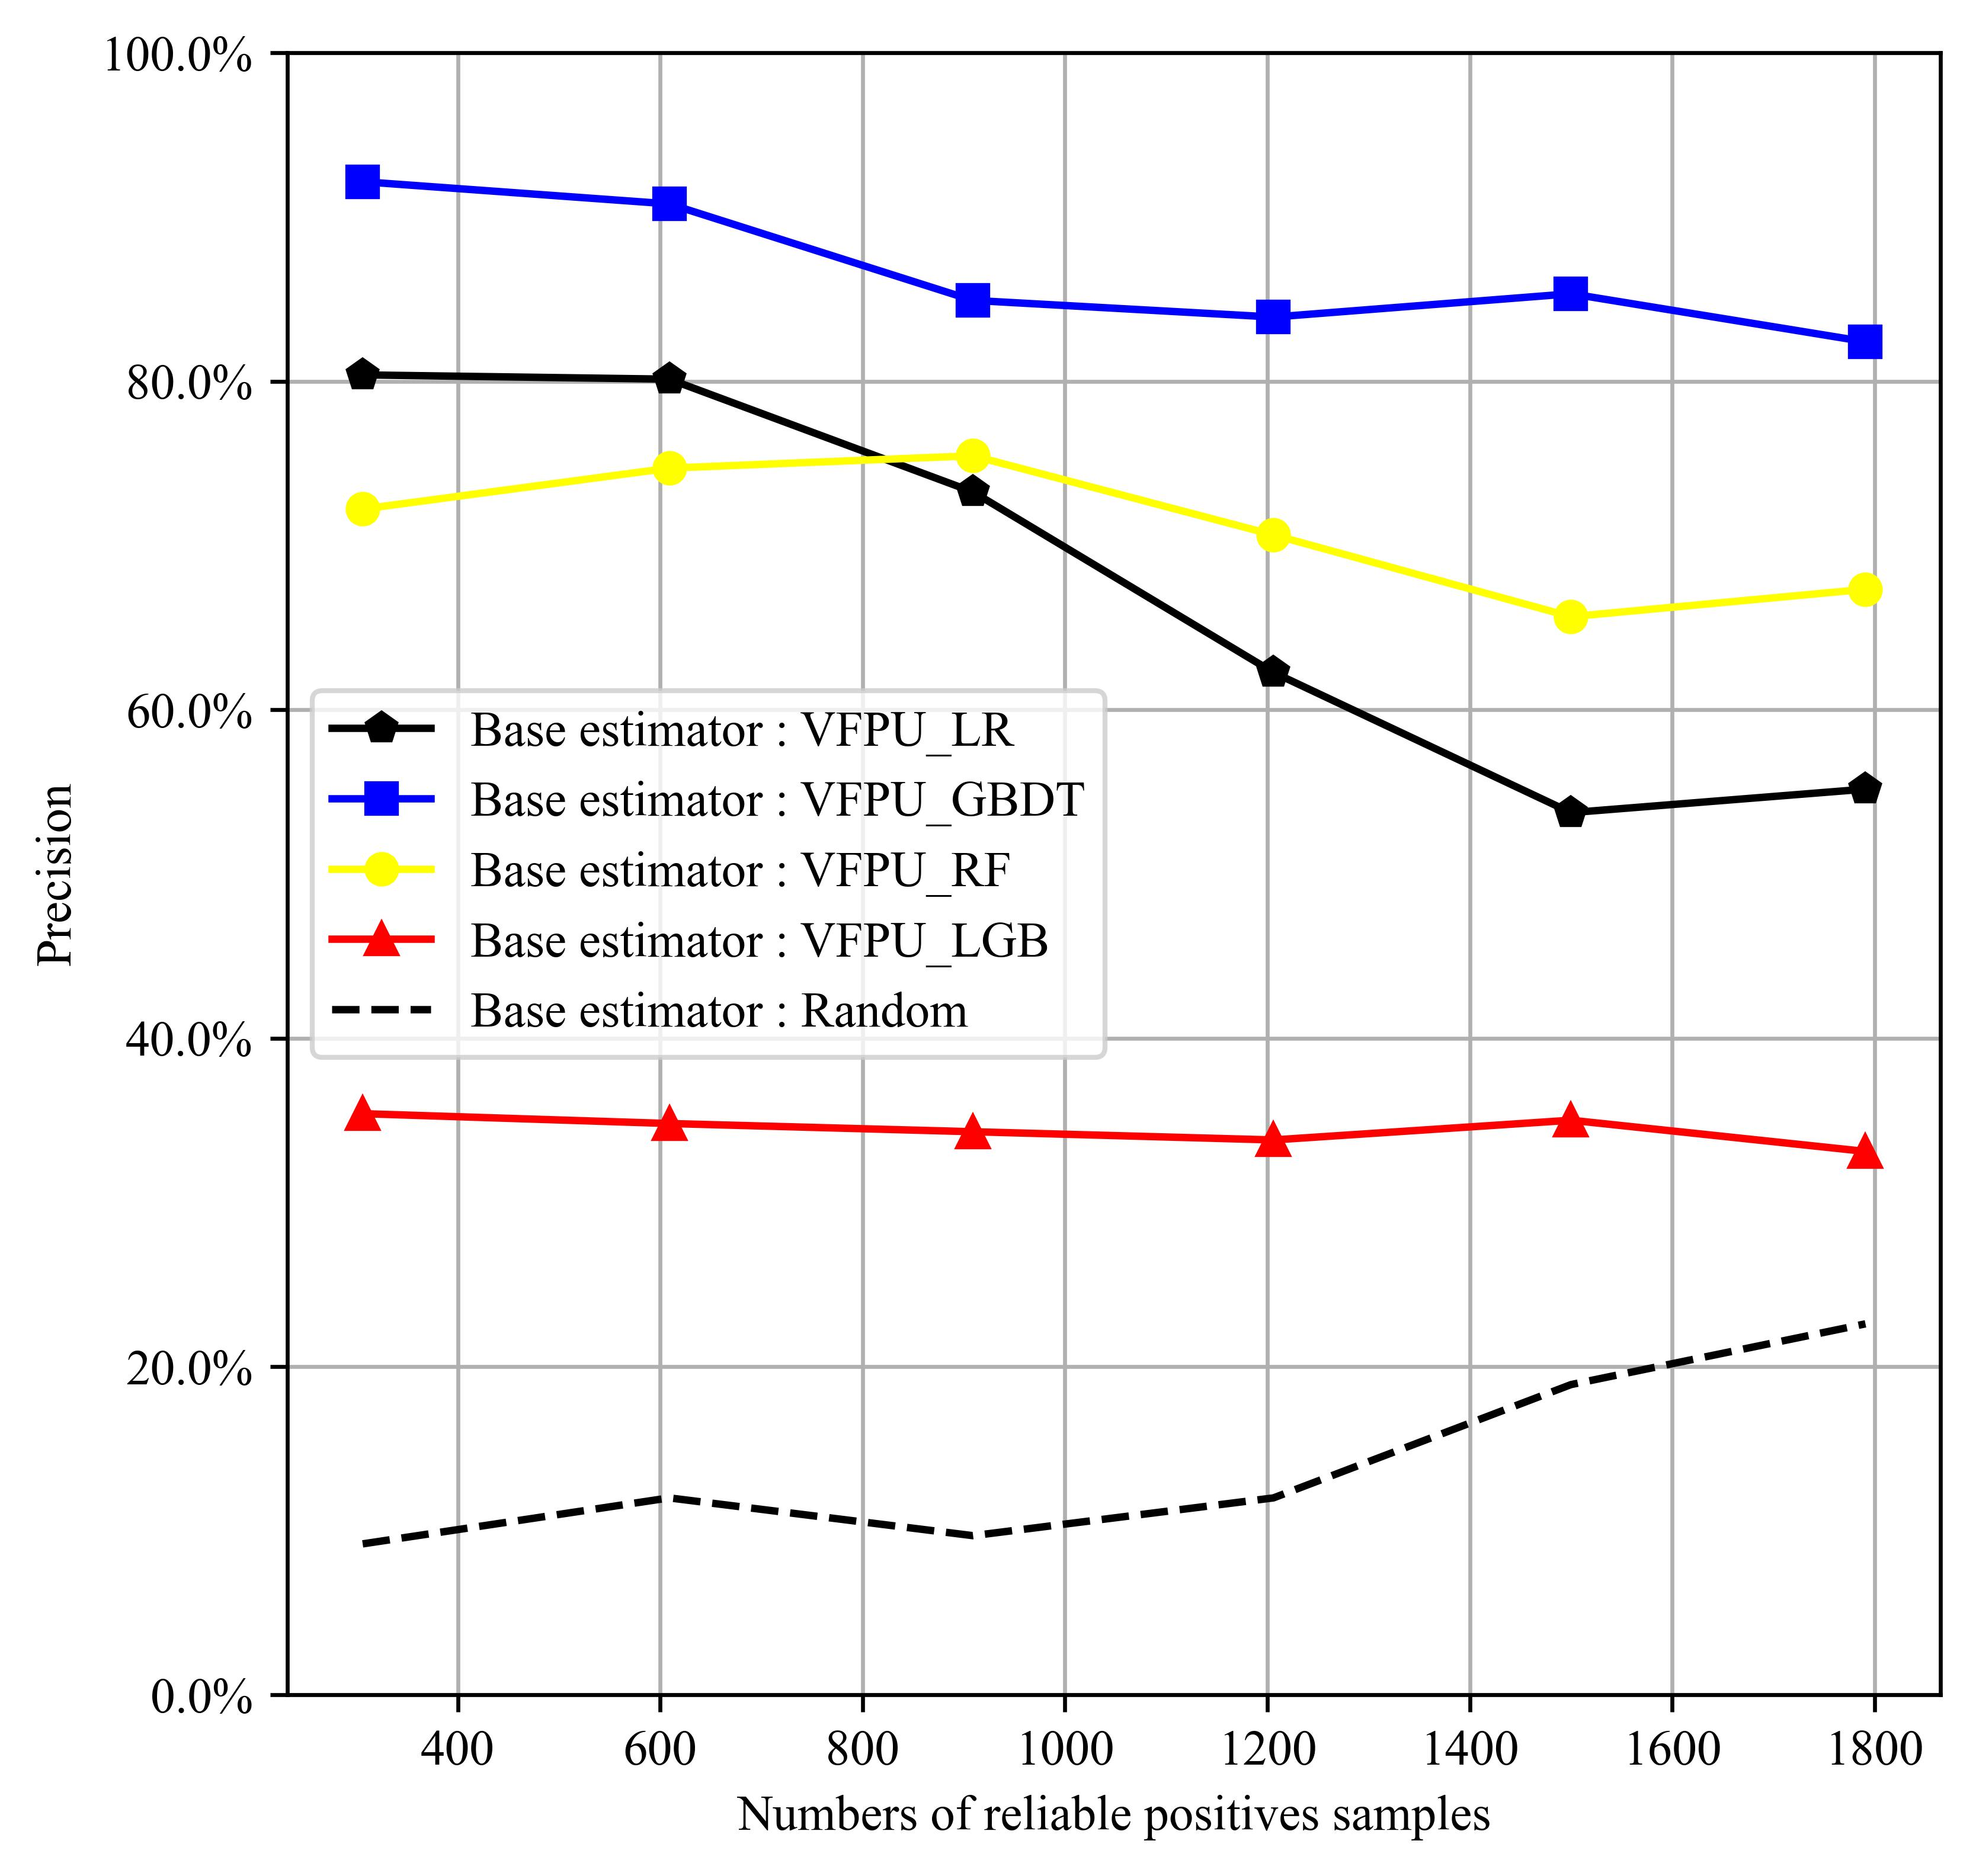
\includegraphics[width=0.9\textwidth,height=5.1cm]{./Figure 4 (1) in JEPG format}
		\caption{Precision}
		\label{RQ2.3.sub1}
	\end{subfigure}
%\hfill
	\begin{subfigure}{0.45\textwidth}
		\centering
		\captionsetup{skip=2pt}
		\captionsetup{size=scriptsize}
		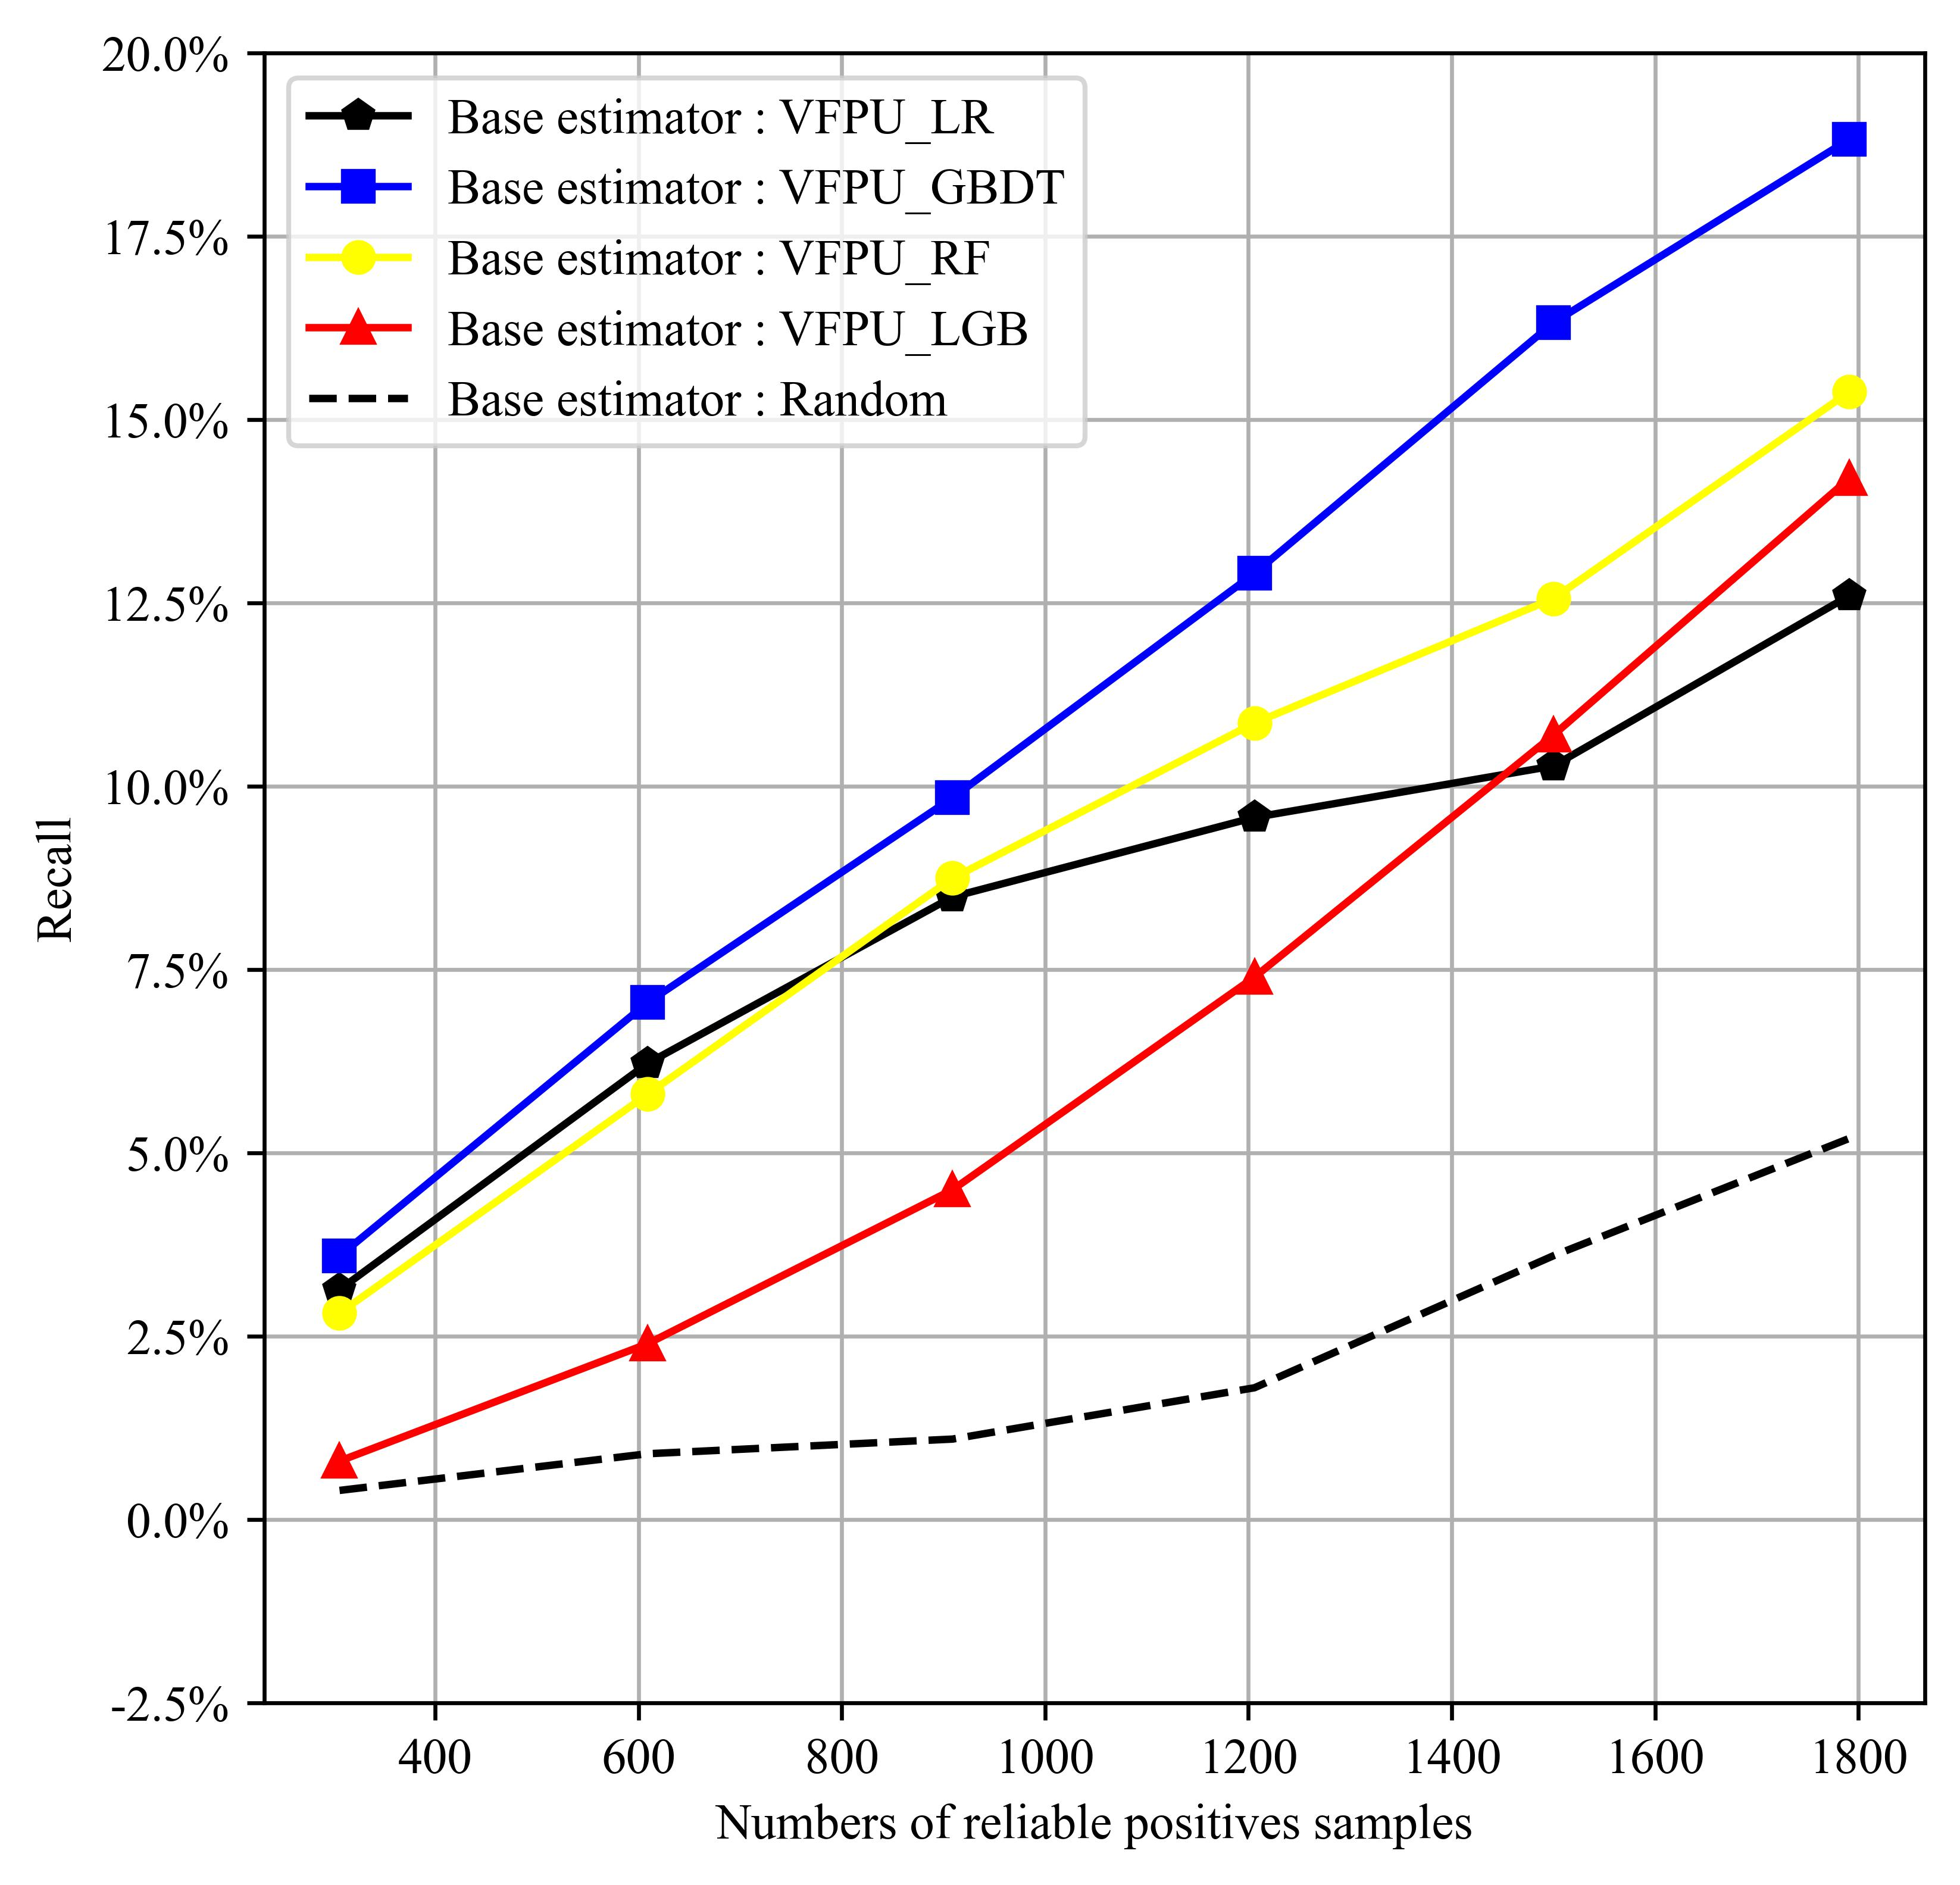
\includegraphics[width=0.9\textwidth,height=5.1cm]{./Figure 4 (2) in JEPG format}
		\caption{Recall}
		\label{RQ2.3.sub2}
	\end{subfigure}
	
%	\vspace{0.05cm}
	
	\begin{subfigure}{0.45\textwidth}
		\centering
		\captionsetup{skip=2pt}
		\captionsetup{size=scriptsize}
		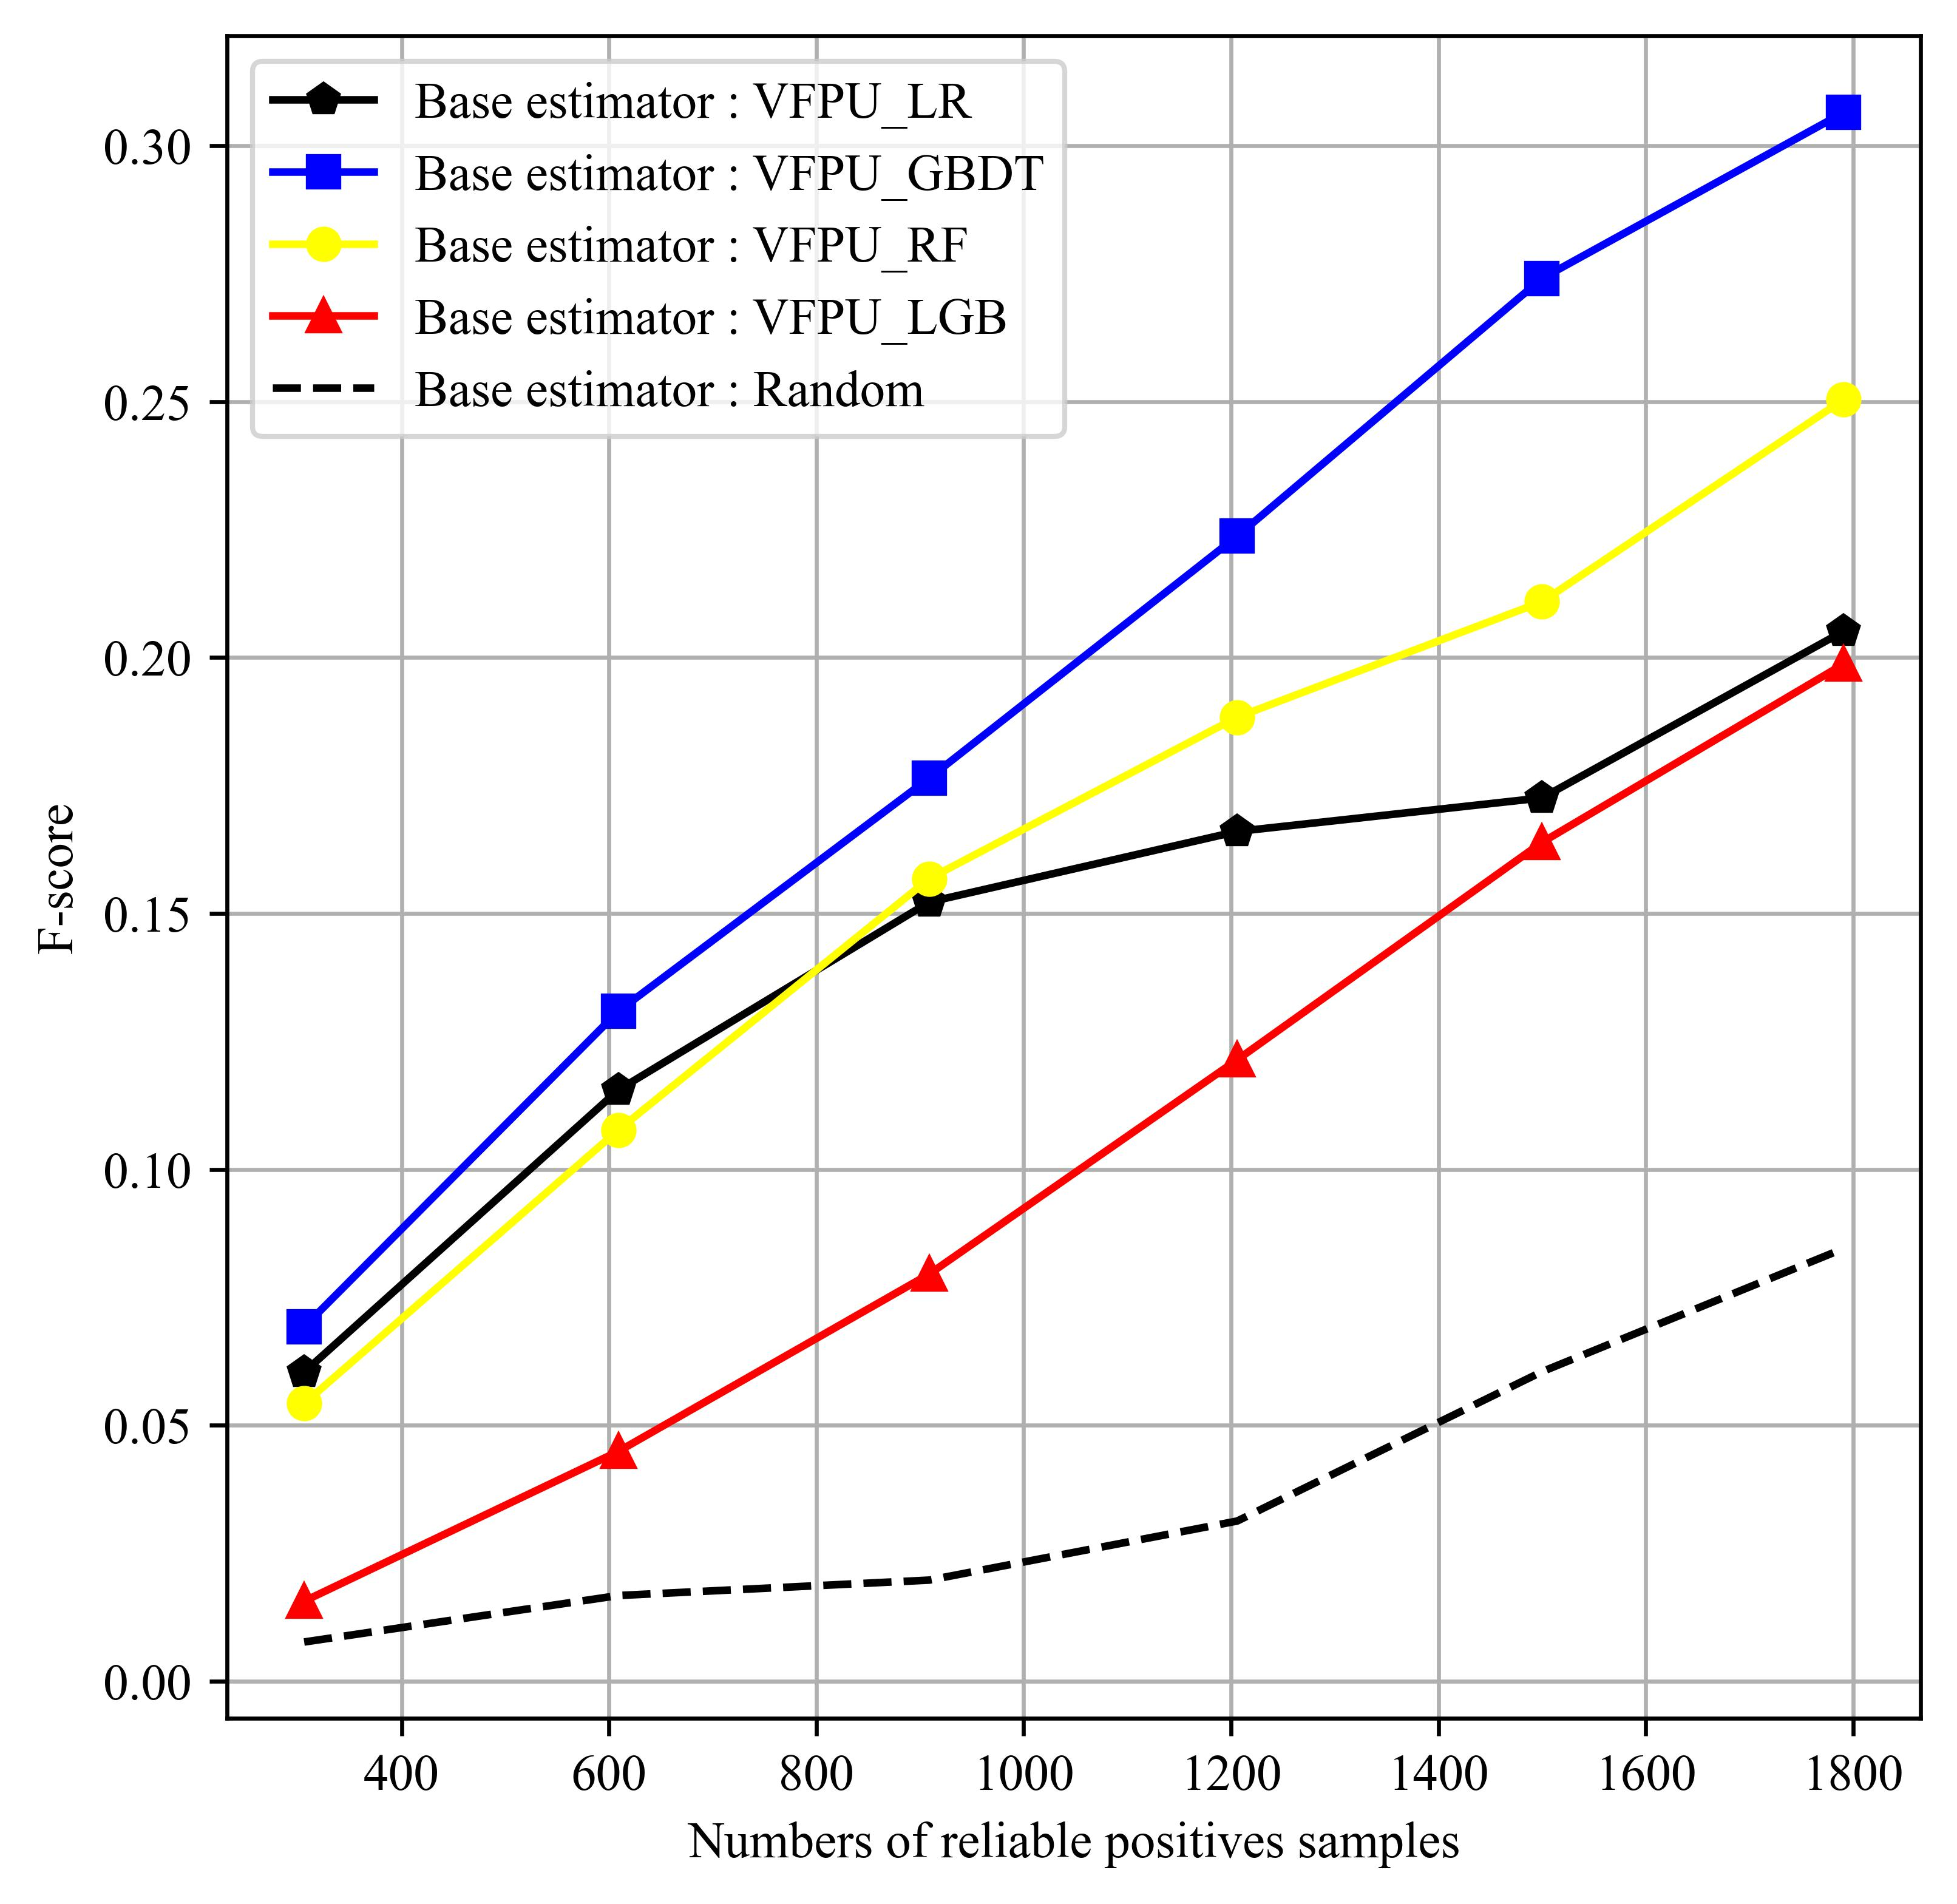
\includegraphics[width=0.9\textwidth,height=5.1cm]{./Figure 4 (3) in JEPG format}
		\caption{F-score}
		\label{RQ2.3.sub3}
	\end{subfigure}
%\hfill
	\begin{subfigure}{0.45\textwidth}
		\centering
		\captionsetup{skip=2pt}
		\captionsetup{size=scriptsize}
		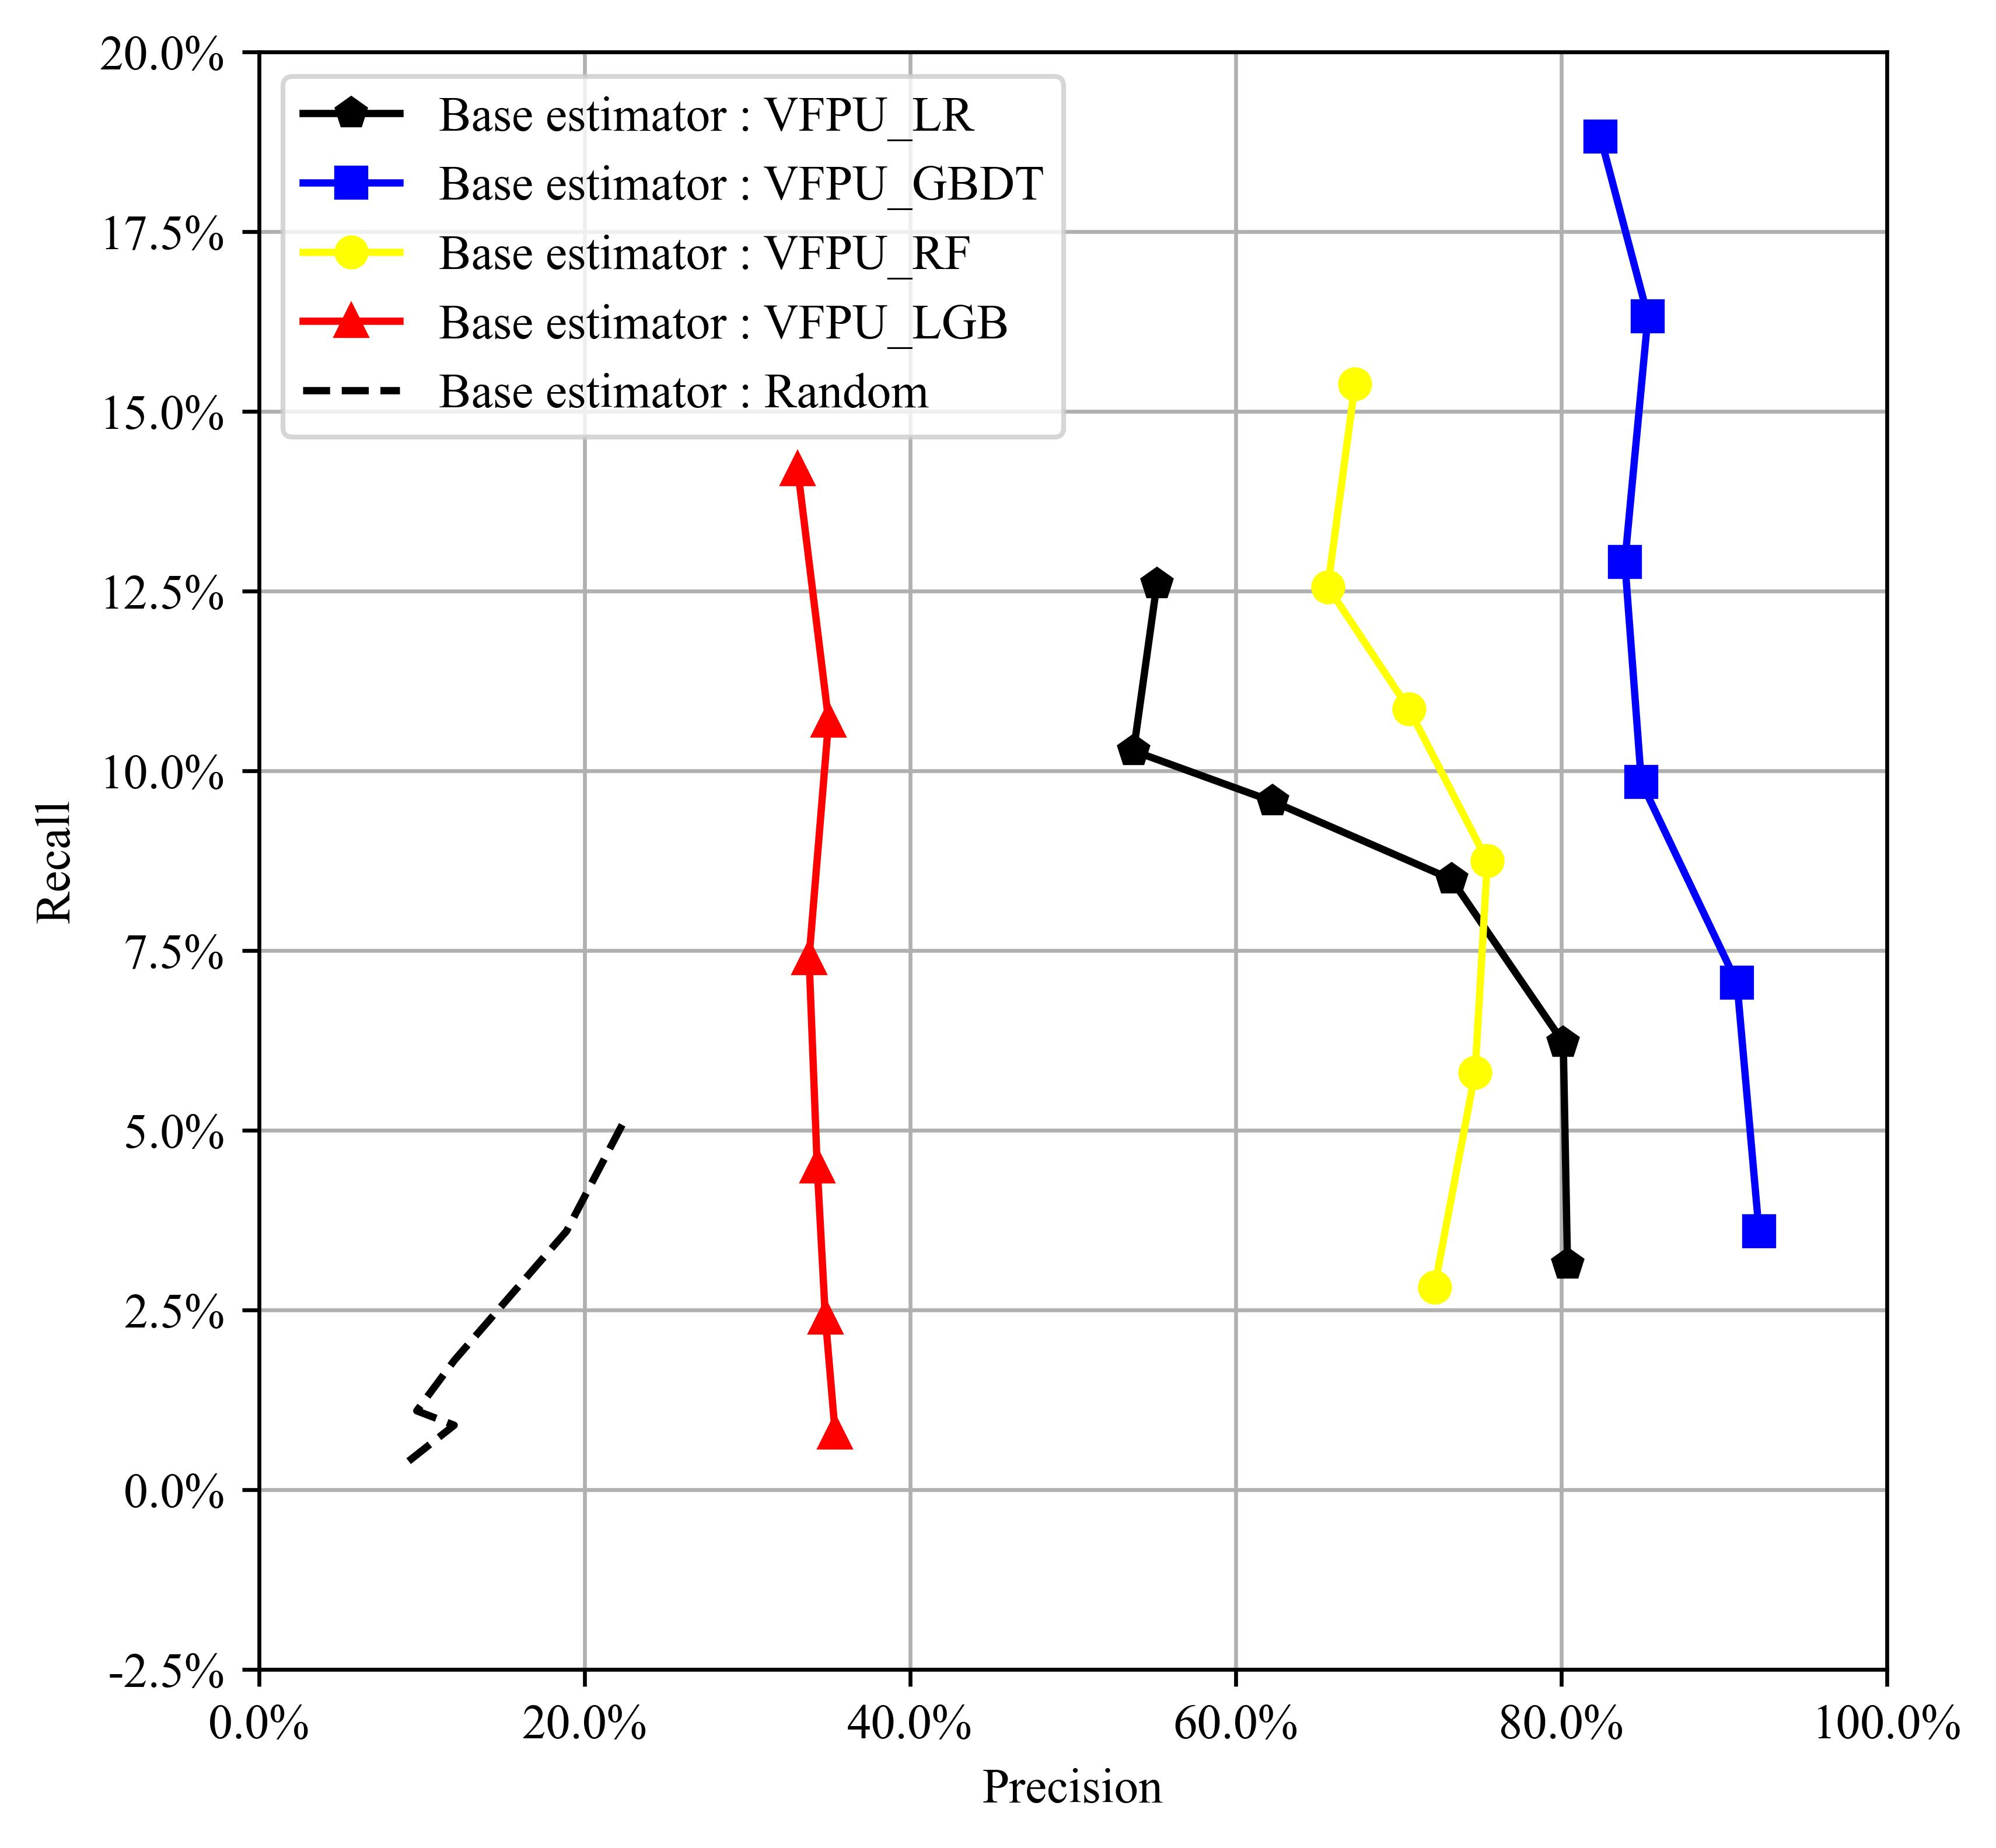
\includegraphics[width=0.9\textwidth,height=5.1cm]{./Figure 4 (4) in JEPG format}
		\caption{Precision-Recall}
		\label{RQ2.3.sub4}
	\end{subfigure}
	
	\caption{Performance of Different Base Estimators with Varying Reliable Positive Samples: (1) Precision; (2) Recall; (3) F-score; (4) Precision-Recall (The Adult Census Dataset)}
	\label{RQ2.3}
\end{figure*}

\begin{figure*}[!htbp]
	\centering
	\captionsetup{size=footnotesize}
	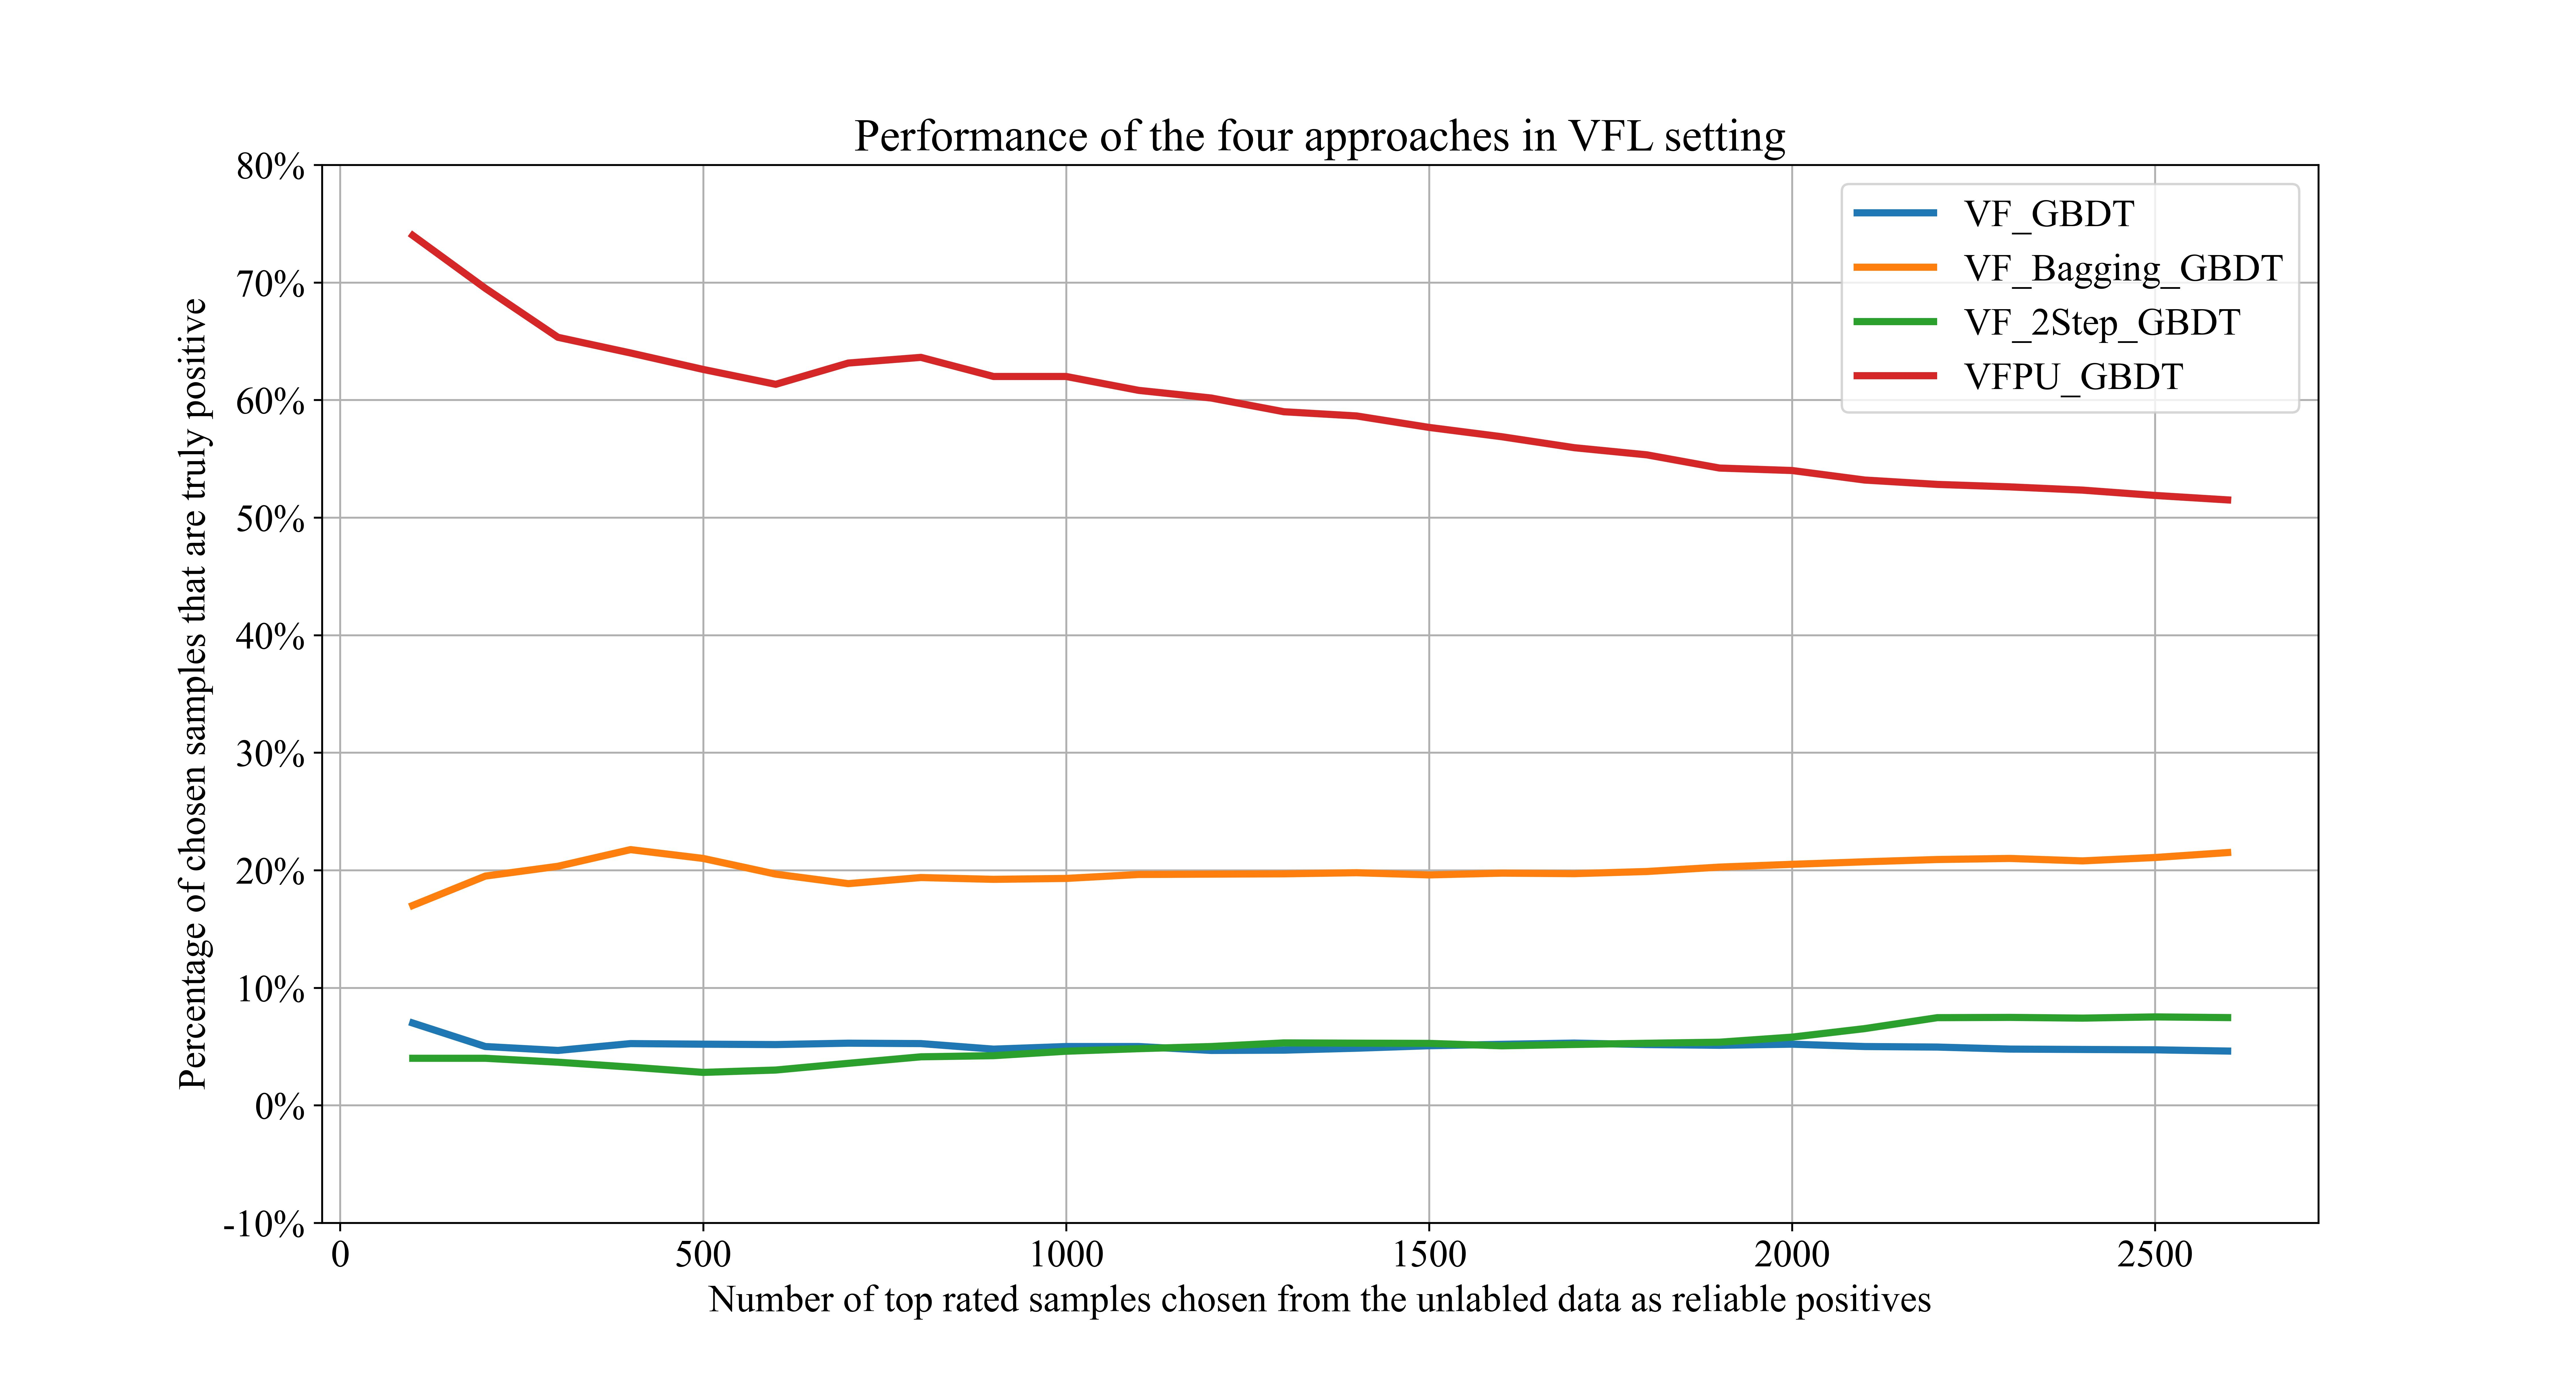
\includegraphics[width=0.9\textwidth,height=9cm]{./Figure 5 in JPEG format}
	\caption{The accurate recommendations percentage by Different Semi-supervised Methods in VFL (The Banking Marketing Dataset)}
	\label{fig:GBDT}
\end{figure*}

\begin{table*}[!htbp]
	\footnotesize
	%	\captionsetup{margin=0.22cm,skip=0pt}
	\caption{The accurate recommendations percentage by different semi-supervised methods (without federation)}
	\label{RQ3.1}
	\begin{tblr}{
			column{3} = {c},
			column{4} = {c},
			column{5} = {c},
			column{6} = {c},
			column{7} = {c},
			column{8} = {c},
			column{9} = {c},
			column{10} = {c},
			column{11} = {c},
			cell{1}{1} = {c=2}{},
			cell{2}{1} = {r=10}{},
			cell{12}{1} = {r=10}{},
			cell{22}{1} = {r=10}{},
			hline{1-2,12,22,32} = {-}{},
		}
		\diagbox{Datasets \& Methods}{$num$} &                                  & 100              & 400              & 700              & 1000             & 1300             & 1600             & 1900             & 2100             & 2400       \\
		 Bank
		& MixMatch                         & 32.81\%          & 32.50\%          & 31.25\%          & 27.97\%          & 24.85\%          & 24.53\%          & 20.31\%          & 13.44\%          & 12.03\%          \\
		& FixMatch                         & 27.81\%          & 27.03\%          & 25.47\%          & 25.16\%          & 24.07\%          & 13.60\%          & 13.28\%          & 12.66\%          & 12.50\%          \\
		& CoMatch                          & 31.56\%          & 27.82\%          & 24.85\%          & 24.69\%          & 24.07\%          & 18.13\%          & 17.19\%          & 12.50\%          & 12.03\%          \\
		& AdaMatch                         & 33.56\%          & 32.97\%          & 30.50\%          & 27.69\%          & 25.78\%          & 22.50\%          & 20.63\%          & 18.13\%          & 17.19\%          \\
		& SoftMatch                        & 32.81\%          & 31.88\%          & 31.56\%          & 25.16\%          & 24.53\%          & 21.88\%          & 19.38\%          & 17.19\%          & 12.50\%          \\
		& \_GBDT                             & 53.65\%          & 50.03\%          & 47.00\%          & 40.20\%          & 33.62\%          & 32.64\%          & 28.99\%          & 29.17\%          & 29.33\%          \\
		& Bagging\_GBDT                    & 42.74\%          & 41.74\%          & 33.46\%          & 29.83\%          & 28.22\%          & 34.65\%          & 31.67\%          & 27.03\%          & 26.00\%          \\
		& 2Step\_GBDT                      & 49.79\%          & 46.66\%          & 42.79\%          & 34.93\%          & 29.72\%          & 33.88\%          & 33.38\%          & 31.30\%          & 26.85\%          \\
		& Pseudo-Labelling                 & 33.30\%          & 22.20\%          & 22.00\%          & 20.90\%          & 21.80\%          & 22.20\%          & 24.10\%          & 23.00\%          & 22.70\%          \\
		& No\_Fed\_VFPU\_GBDT (Our Method) & \textbf{77.00\%} & \textbf{68.25\%} & \textbf{66.86\%} & \textbf{63.80\%} & \textbf{59.62\%} & \textbf{57.63\%} & \textbf{54.26\%} & \textbf{53.95\%} & \textbf{52.38\%} \\
		
		
		Credit
		& MixMatch                         & 29.29\%          & 25.75\%          & 25.34\%          & 25.34\%          & 24.09\%          & 24.09\%          & 23.88\%          & 23.47\%          & 21.18\%          \\
		& FixMatch                         & 27.00\%          & 25.55\%          & 25.34\%          & 24.30\%          & 23.88\%          & 23.47\%          & 22.85\%          & 22.43\%          & 21.39\%          \\
		& CoMatch                          & 26.79\%          & 25.75\%          & 25.55\%          & 24.92\%          & 24.09\%          & 23.88\%          & 23.47\%          & 22.85\%          & 21.18\%          \\
		& AdaMatch                         & 26.79\%          & 26.79\%          & 25.34\%          & 25.13\%          & 25.13\%          & 24.09\%          & 22.85\%          & 22.63\%          & 21.18\%          \\
		& SoftMatch                        & 26.38\%          & 25.55\%          & 24.09\%          & 23.88\%          & 23.47\%          & 22.85\%          & 22.43\%          & 21.18\%          & 20.97\%          \\
		& \_GBDT                             & 42.80\%          & 38.21\%          & 34.62\%          & 30.67\%          & 31.56\%          & 29.30\%          & 29.89\%          & 28.65\%          & 25.43\%          \\
		& Bagging\_GBDT                    & 42.74\%          & 32.86\%          & 30.40\%          & 26.72\%          & 25.52\%          & 27.48\%          & 26.17\%          & 26.91\%          & 24.55\%          \\
		& 2Step\_GBDT                      & 42.74\%          & 39.50\%          & 33.29\%          & 30.17\%          & 31.77\%          & 31.97\%          & 26.24\%          & 27.57\%          & 26.00\%          \\
		& Pseudo-Labelling                 & 38.40\%          & 37.00\%          & 32.50\%          & 32.30\%          & 30.90\%          & 30.30\%          & 29.20\%          & 28.40\%          & 27.30\%          \\
		& No\_Fed\_VFPU\_GBDT (Our Method) & \textbf{51.25\%} & \textbf{50.83\%} & \textbf{50.14\%} & \textbf{48.50\%} & \textbf{47.69\%} & \textbf{45.88\%} & \textbf{41.82\%} & \textbf{40.82\%} & \textbf{39.82\%} \\
		
		
		Census
		& MixMatch                         & 37.72\%          & 37.06\%          & 36.39\%          & 35.94\%          & 36.05\%          & 35.49\%          & 34.15\%          & 32.81\%          & 32.59\%          \\
		& FixMatch                         & 38.84\%          & 38.61\%          & 37.28\%          & 37.06\%          & 36.39\%          & 35.71\%          & 34.38\%          & 33.93\%          & 32.36\%          \\
		& CoMatch                          & 37.18\%          & 36.51\%          & 34.06\%          & 33.39\%          & 32.97\%          & 32.49\%          & 31.38\%          & 31.38\%          & 31.38\%          \\
		& AdaMatch                         & 38.39\%          & 38.39\%          & 37.50\%          & 37.28\%          & 36.24\%          & 35.81\%          & 35.49\%          & 34.38\%          & 33.93\%          \\
		& SoftMatch                        & 38.84\%          & 37.28\%          & 35.94\%          & 35.86\%          & 35.04\%          & 34.15\%          & 33.93\%          & 32.81\%          & 29.91\%          \\
		& \_GBDT                             & 64.00\%          & 64.00\%          & 61.00\%          & 64.00\%          & 58.00\%          & 57.00\%          & 54.00\%          & 51.00\%          & 54.00\%          \\
		& Bagging\_GBDT                    & 68.00\%          & 58.00\%          & 59.00\%          & 55.00\%          & 54.00\%          & 49.00\%          & 52.00\%          & 48.00\%          & 51.00\%          \\
		& 2Step\_GBDT                      & 66.00\%          & 68.00\%          & 63.00\%          & 62.00\%          & 56.00\%          & 58.00\%          & 51.00\%          & 52.00\%          & 53.00\%          \\
		& Pseudo-Labelling                 & 42.90\%          & 39.70\%          & 29.30\%          & 39.90\%          & 28.40\%          & 44.50\%          & 41.40\%          & 37.30\%          & 45.30\%          \\
		& No\_Fed\_VFPU\_GBDT (Our Method) & \textbf{99.00\%} & \textbf{99.25\%} & \textbf{99.43\%} & \textbf{99.00\%} & \textbf{94.57\%} & \textbf{88.50\%} & \textbf{84.08\%} & \textbf{80.08\%} & \textbf{75.08\%} 
		
	\end{tblr}
\end{table*}










\begin{table*}[!htbp]
	\footnotesize
	%	\captionsetup{margin=0.43cm,skip=0pt}
	\caption{The accurate recommendations percentage by different semi-supervised methods (in VFL) }
	\label{RQ3.2}
	\begin{adjustbox}{max width=\textwidth,center}
	\begin{tblr}{
			% 合并单元格操作
			cell{1}{1} = {c=2}{},
			cell{2}{1} = {r=4}{},
			cell{6}{1} = {r=4}{},
			cell{10}{1} = {r=4}{},
			hline{1-2,14} = {-}{},			
		}
	
		% 表头
		\diagbox{Datasets \& Methods}{$num$} &               & 100     & 400     & 700     & 1000    & 1300    & 1600    & 1900    & 2100    & 2400   &runtime(s) \\
		
		 Bank
		& VF\_GBDT                          & 7.00\%           & 5.30\%           & 5.30\%           & 5.00\%           & 4.70\%           & 5.20\%           & 5.10\%           & 5.00\%           & 4.80\%           & 10673.81          \\
		& VF\_Bagging GBDT                  & 17.00\%          & 21.80\%          & 18.90\%          & 19.30\%          & 19.70\%          & 19.80\%          & 20.30\%          & 20.70\%          & 20.80\%          & 15069.88          \\
		& VF\_2Step GBDT                    & 4.00\%           & 3.30\%           & 3.60\%           & 4.60\%           & 5.30\%           & 5.10\%           & 5.40\%           & 6.50\%           & 7.40\%           & 44030.4           \\
		& VFPU\_GBDT (Our Method) & \textbf{74.00\%} & \textbf{64.00\%} & \textbf{63.10\%} & \textbf{62.00\%} & \textbf{59.00\%} & \textbf{56.90\%} & \textbf{54.20\%} & \textbf{53.20\%} & \textbf{52.30\%} & \textbf{106922.2} \\
		
		Credit
		& VF\_GBDT                          & 18.00\%          & 22.50\%          & 22.60\%          & 22.50\%          & 22.10\%          & 21.80\%          & 21.40\%          & 21.60\%          & 22.30\%          & 12025.47          \\
		& VF Bagging GBDT                  & 32.00\%          & 27.50\%          & 23.90\%          & 23.60\%          & 23.50\%          & 23.40\%          & 23.30\%          & 22.30\%          & 22.00\%          & 15791.59          \\
		& VF\_2Step GBDT                    & 24.00\%          & 26.30\%          & 25.40\%          & 23.90\%          & 23.70\%          & 23.10\%          & 22.30\%          & 22.30\%          & 22.00\%          & 46954.19          \\
		& VFPU\_GBDT (Our Method) & \textbf{44.00\%} & \textbf{50.25\%} & \textbf{48.86\%} & \textbf{46.50\%} & \textbf{44.85\%} & \textbf{41.88\%} & \textbf{39.47\%} & \textbf{38.33\%} & \textbf{37.43\%} & \textbf{107075.9} \\
		
		Census
		& VF\_GBDT                          & 19.00\%          & 24.50\%          & 25.40\%          & 24.20\%          & 23.90\%          & 23.60\%          & 23.10\%          & 22.90\%          & 22.80\%          & 11581.47          \\
		& VF\_Bagging GBDT                  & 13.00\%          & 18.00\%          & 19.90\%          & 21.10\%          & 22.30\%          & 23.30\%          & 23.20\%          & 23.20\%          & 23.90\%          & 15987.59          \\
		& VF\_2Step GBDT                    & 25.00\%          & 23.30\%          & 23.10\%          & 23.40\%          & 24.30\%          & 24.10\%          & 24.60\%          & 25.00\%          & 25.60\%          & 46808.19          \\
		& VFPU\_GBDT (Our Method) & \textbf{98.00\%} & \textbf{99.00\%} & \textbf{98.71\%} & \textbf{98.70\%} & \textbf{94.23\%} & \textbf{87.25\%} & \textbf{80.53\%} & \textbf{76.05\%} & \textbf{72.74\%} & \textbf{107089.9}   
	
	
\end{tblr}
\end{adjustbox}
\end{table*}


\subsubsection{RQ3: Uncovering hidden positive samples: VFPU vs. other semi-supervised methods in VFL Setting}

To assess the effectiveness of our method in addressing the UDD-PU problem, we conducted two experiments to compare it with other semi-supervised learning methods. The first experiment identifies the most effective semi-supervised methods for solving PU problems, which serve as the foundation for UDD-PU problems but without federation. The second experiment compares the top four semi-supervised methods from the first experiment in addressing the UDD-PU problem in VFL.


In the first experiment, we compared No\_Fed\_VFPU\_GBDT with other 9 semi-supervised learning methods without federation, and the results are presented in \autoref{RQ3.1}. The compared methods include a direct application of GBDT \cite{elkan2008learning} (denoted as \_GBDT), Bagging\_GBDT \cite{mordelet2014bagging}, 2Step\_GBDT \cite{liu2003building}, Pseudo-labeling \cite{lee2013pseudo}, MixMatch \cite{berthelot2019mixmatch},  FixMatch \cite{sohn2020fixmatch}, CoMatch \cite{li2021comatch}, AdaMatch \cite{berthelot2021adamatch} and SoftMatch \cite{chen2023softmatch}.
\begin{quote}
	\textbf{\_GBDT:} directly applies a GBDT classifier to the PU data with unlabeled data (U) treated as negative samples and labeled data (P) treated as positive samples.
\end{quote}

\begin{quote}
	\textbf{Bagging\_GBDT:} an ensemble method that utilizes the bagging technique for PU learning. It repeatedly samples from the unlabeled dataset to create diverse training sets, each containing a mixture of positive and unlabeled samples. A GBDT classifier is trained on each of these sets and the final prediction is obtained by averaging the predictions of all classifiers.
\end{quote}

\begin{quote}
	\textbf{2Step\_GBDT:} firstly, trains a GBDT classifier on the positive and unlabeled samples, treating all unlabeled samples as negative. In the second step, the GBDT classifier is retrained on a subset of the unlabeled data that is most likely to contain hidden positive samples, identified based on their predicted probabilities in the first step.
\end{quote}

\begin{quote}
	\textbf{Pseudo-labeling:} a semi-supervised learning technique that involves using the predictions of a model on unlabeled data to create pseudo-labels for that data. These pseudo-labels are then combined with the labeled data to train a new model or improve the existing model.
\end{quote}

\begin{quote}
	\textbf{MixMatch:} guesses low-entropy labels for data-augmented unlabeled examples and mixes labeled and unlabeled data using MixUp \cite{zhang2017mixup}. We set $T = 0.5$ and $K = 2$.
\end{quote}

\begin{quote}
	\textbf{FixMatch:} is the upgraded version of Pseudo Labeling. FixMatch turns the predictions on weakly-augmented unlabeled data into hard 'one-hot' pseudo-labels and then further uses them as the learning signal of strongly-augmented unlabeled data. We use a set of hyperparameters($\tau = 0.95, \nu = 7, B = 64$).
\end{quote}

\begin{quote}
	\textbf{CoMatch:} learns two representations of training data, class probabilities and low dimensional embeddings, which interact with each other to improve pseudo-labels through a smoothness constraint and regularize the structure of the embeddings using graph-based contrastive learning. We follow FixMatch \cite{sohn2020fixmatch} and set the same hyperparameters.
\end{quote}

\begin{quote}
	\textbf{AdaMatch:} is proposed mainly for domain adaption, but can also adapted to SSL. It is characterized by relative threshold and distribution alignment, where the relative threshold is adaptively estimated from EMA \cite{tarvainen2017mean} of the confidence on labeled data. The confidence threshold $\tau$ is set to 0.9.
\end{quote}

\begin{quote}
	\textbf{SoftMatch:} maintains both high quantity and quality of pseudo-labels during training, weighting samples based on their confidence through a truncated Gaussian function, and enhances the utilization of weakly-learned classes with a uniform alignment approach. We set $m$ to 0.999 and divide the estimated variance ${{\hat \sigma }_t}{\kern 1pt} {\kern 1pt} {\kern 1pt}$ by 4 for $2\sigma$ of the Gaussian function.
\end{quote}

 In the first experiment, we scored all unlabeled samples using a classifier, and these scores represented the probability that the sample would be predicted as positive. We then ranked these scores and labeled the higher ranked samples as top-rated. The number of unlabeled samples chosen from top-rated is denoted as $num$ as shown in \autoref{RQ3.1}. We set the coefficient of the L2 penalty term to 0.4, the learning rate to 0.0002, and the batch size to 32 for the LR algorithm. For decision tree algorithms, the number of trees is set to 500, and the tree depth is set to 12. The learning rate is set to 0.02. We use the Wide ResNet-28 model from \cite{oliver2018realistic} for FixMatch, CoMatch, AdaMatch, and SoftMatch.

\autoref{RQ3.1} demonstrates that our method No\_Fed\_VFPU\_GBDT outperforms other nine semi-supervised methods across all datasets and different $num$ in uncovering hidden positive samples without federation. For instance, on the Census dataset, when $num=1000$, in the term methods, No\_Fed\_VFPU\_GBDT achieves the highest recommendation accuracy of 99\%. This is followed by \_GBDT, 2Step\_GBDT, and Baggin\_GBDT with accuracies of 64\%, 62\%, and 55\% respectively. The recommendation accuracies for MixMatch, FixMatch, CoMatch, AdaMatch, and SoftMatch are 35.94\%, 37.06\%, 33.39\%, 37.28\%, and 35.86\% respectively.

The Match series algorithms (FixMatch, CoMatch, AdaMatch, and SoftMatch), despite being the most recent, underperform compared to other semi-supervised learning methods in solving the PU problem. The reason for the underperformance could be: a) these methods still require labeled data for negative samples which are absent in the PU problem; b) these methods chose wide-resnet, a complex deep learning network, which may induce overfitting in data with extremely unbalanced samples.


The PU learning methods (VFPU\_GBDT, \_GBDT, Bagging\_GBDT, 2Step\_GBDT) in our specific scenario are capable of uncovering more potential positive samples. The top four methods as illustrated in \autoref{RQ3.1} are \_GBDT, Bagging\_GBDT, 2Step\_GBDT and VFPU\_GBDT. 

In the second experiment, we adapted the top four methods from the first experiment for a Vertical Federated Learning (VFL) setting, denoted as VF\_GBDT, VF\_Bagging\_GBDT, VF\_2Step\_GBDT, and VFPU\_GBDT. Meanwhile, to evaluate the time complexity of these methods in VFL setting, we recorded the training time for each method across diverse datasets when $num = 2400$. The traning time is denoted as runtime(s), with 's' indicating seconds in \autoref{RQ3.2}.
 

\autoref{RQ3.2}, similar to \autoref{RQ3.1}, compares the accuracy percentages of different methods but  in the VFL setting. The results in \autoref{RQ3.2} clearly show that the VFPU\_GBDT method surpasses other methods. For example, on the Census dataset, with $num=1000$, VFPU\_GBDT achieves a high recommendation accuracy of 98.70\%, significantly outperforming VF\_GBDT, VF\_Bagging\_GBDT, and VF\_2Step\_GBDT, which achieve accuracies of 24.20\%, 21.10\%, and 24.30\% respectively. On the Credit dataset, our method had a runtime of 107075.9s, while the runtimes for the other three methods were 12025.47s, 15791.59s, and 46954.19s respectively.
VFPU\_GBDT is approximately 10 times more time-consuming than other methods in terms of the metric of runtime(s). This is because VFPU adopts a more cautious strategy in selecting reliable positive samples through multiple iterations, and selecting only a small portion in each iteration. So there is a trade-off between the training time and the accuracy of the recommandation, and this time overhead is absolutely acceptable since the accuracy is significantly improved.

\autoref{fig:GBDT} visualizes the results of the Bank Marketing Dataset in \autoref{RQ3.2}. In \autoref{fig:GBDT}, the x-axis represents the varying amounts of top-rated unlabeled samples chosen as reliable positive samples. The y-axis denotes the percentage of these selected samples that are truly positive. The figure shows that the number of hidden positive samples identified by VFPU\_GBDT decreases rapidly as $num$ ranges from 100 to 1000. This decrease is attributed to several factors. First, unlabeled data samples that exhibit apparent similarity or difference form the positive samples are easily identified quickly. Then, the rest unlabeled data thatexhibit feature overlap between both classes introduce more interference to the classifier. This interference leads to misclassification and the percentage of accurate recommendation decreases. While other methods appear relatively stable, this stability is not necessarily advantageous. The accurate recommnedation percentage of other methods in identifying hidden positive samples is generally low. Regardless of the quantity of unlabeled samples selected from the top rated, they consistently fail to achieve satisfactory accuracy. In the experiment setup, there are only about 2500 true positive samples in this unlabeled dataset. Therefore, the accuracy of VFPU\_GBDT is decreasing when the number of selected positive samples exceeds 2500.
 
In summary, the effectiveness of the VFPU\_GBDT algorithm in recommending reliable positive samples in a VFL environment outperforms other semi-supervised methods. This experiment highlights the benefits of using the VFPU\_GBDT algorithm to address the unlabeled data-deficient PU (UDD-PU) learning recommendation problem in a federated learning environment.




\section{Conclusion}
\label{sec5}

This paper posed the Unlabeled-Data-Deficient PU (UDD-PU) learning problem in recommender systems, where the party requiring the recommendation service holds only positive data while other parties possess abundant unlabeled data. To address the UDD-PU problem, a multi-party federated recommendation method based on semi-supervised learning was proposed. Specifically, we designed the VFPU algorithm as the core of the method, which effectively integrated two PU learning techniques and then adapted it into a vertical federated learning framework. In this way, VFPU was able to utilize limited labeled data (positive samples) and abundant unlabeled data to improve the performance of the recommendation model. We evaluated our proposed method on three datasets and compared it with other semi-supervised leaning methods. The experimental results evidently demonstrated that the VFPU algorithm can achieve satisfactory performance with little degradation compared to non-federated methods while ensuring data privacy. Additionally, we showed that the VFPU algorithm consistently outperforms other semi-supervised learning methods in uncovering hidden positive samples within the vertical federated learning context. Moreover, the analysis of different base estimators revealed that Gradient Boosting Decision Trees (VFPU\_GBDT) consistently delivered superior performance in terms of precision, recall, and F-score. This finding highlights the importance of selecting an appropriate base estimator for the VFPU algorithm so as to optimize its performance in various real-world applications.


Although VFPU has shown good performance in solving the UDD-PU problem, there are still some limitations: First, the strategy of the VFPU method in handling unaligned samples needs to be improved. The current strategy is to directly discard these samples, which is based on \cite{yang2019federated}. However, this may lose information in those unaligned samples that is valuable for classification. Therefore, our future work will explore how to utilize these unaligned samples more efficiently in order to fully exploit their potential in classification problems. Second, the VFPU method is currently only applicable to binary classification PU problems. However, in some cases, we face a multiple-positive-multiple-negative PU (MPMN-PU) learning problem \cite{lin2022federated}. Therefore, extending the VFPU method to handle MPMN-PU problems will be another important direction for our future research.



\section*{Acknowledgments}
This work was supported by Soft Science Research Project of Ministry of Housing and Urban-Rural Development of the People’s Republic of China under Grant No. 2022-R-004; Chongqing Construction Science and technology plan project of Chongqing Housing and Urban-Rural Development Commission under Grant No. CKZ 2021 2-9; the Doctoral Direct Train project of Chongqing Science and Technology Bureau under Grant No. CSTB2022BSXM-JSX0007.

%\clearpage
\bibliographystyle{IEEEtranN}
\bibliography{references}

\begin{IEEEbiography}[{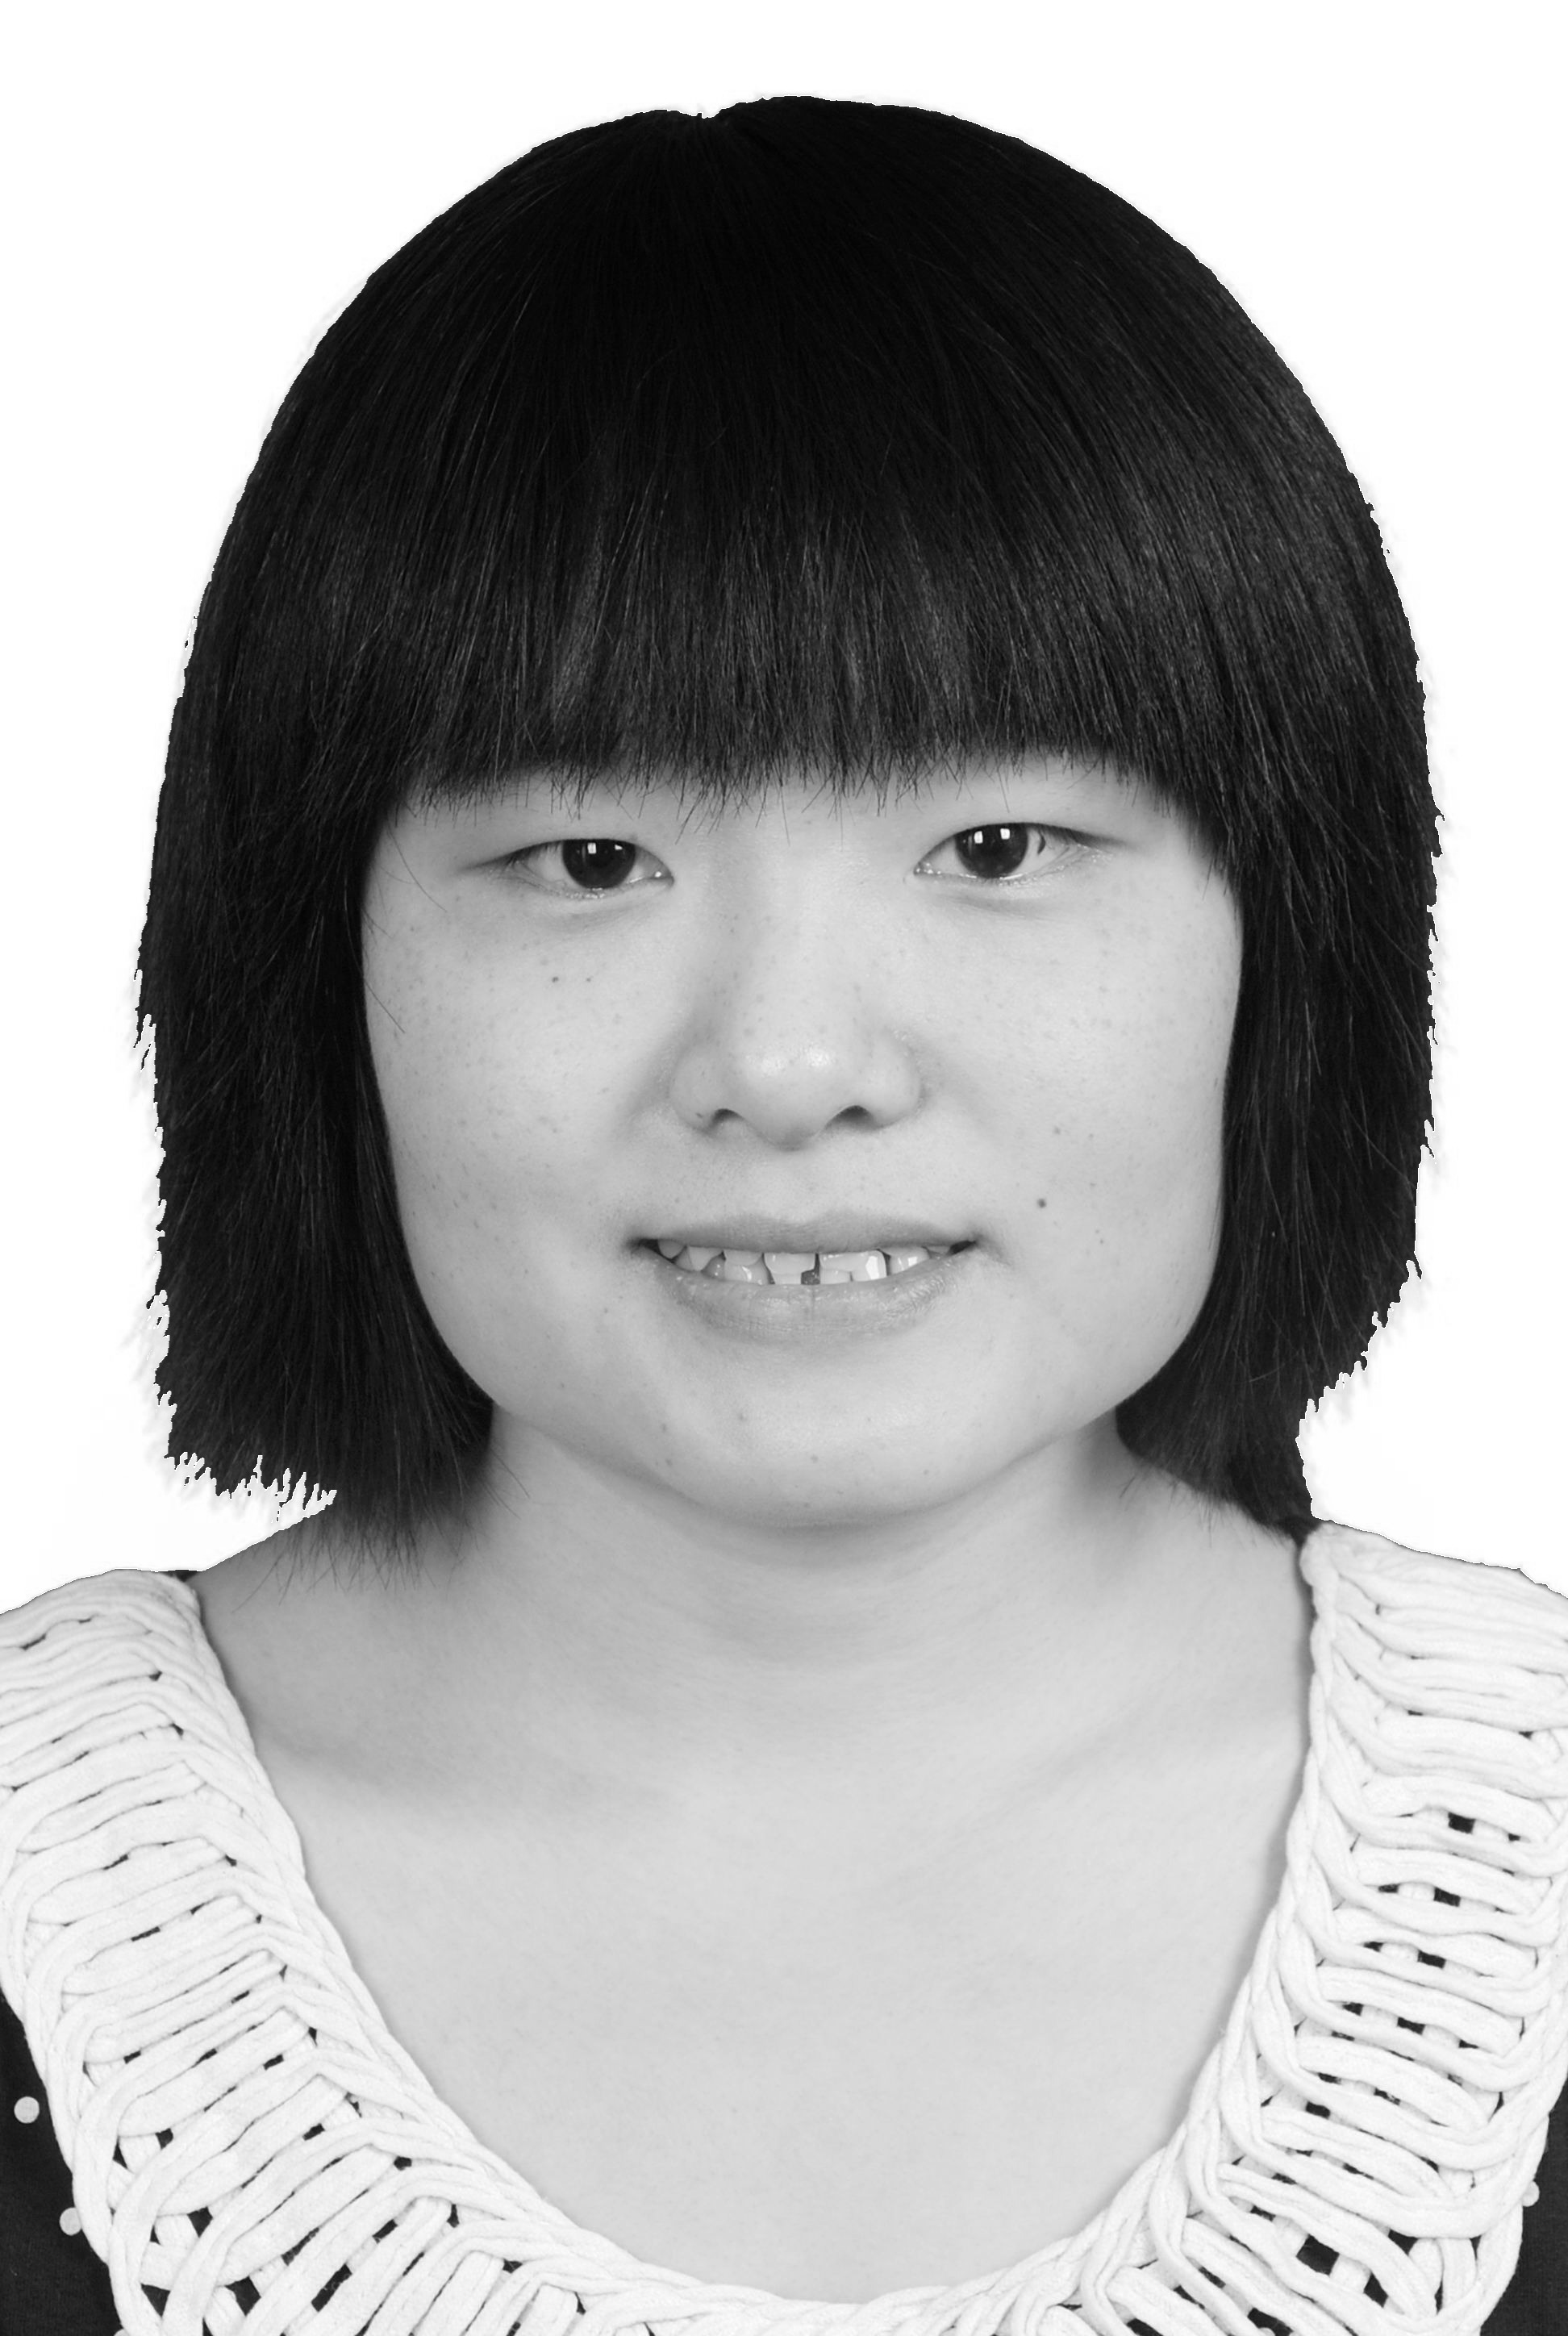
\includegraphics[width=1in,height=1.25in,clip,keepaspectratio]{liuxin}}]{Xin liu}
	received the Ph.D. degree in computer science from Chongqing University, in 2012. She is an associate professor in School of Software Engineering, Chongqing University of Posts and Telecommunications. Her current research interests include machine learning, data analysis, and video/image processing.
\end{IEEEbiography}


\begin{IEEEbiography}[{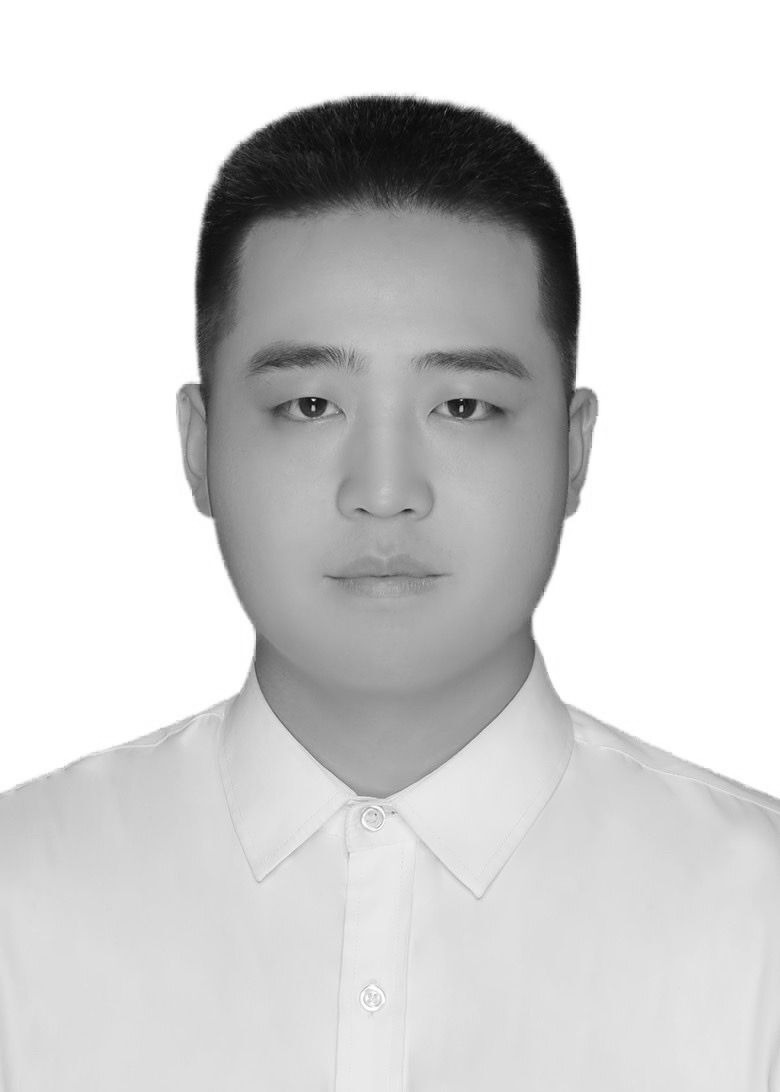
\includegraphics[width=1in,height=1.25in,clip,keepaspectratio]{lvjiuluan}}]{Jiuluan Lv}
	received the BS degree from the Chongqing Jiaotong University, Chongqing, China, in 2022. He is currently working toward the master's degree with Chongqing University of Posts and Telecommunications, Chongqing, China. His reseach interests include federated learning, deep learning, data mining, and data analysis, etc. 
\end{IEEEbiography}


\begin{IEEEbiography}[{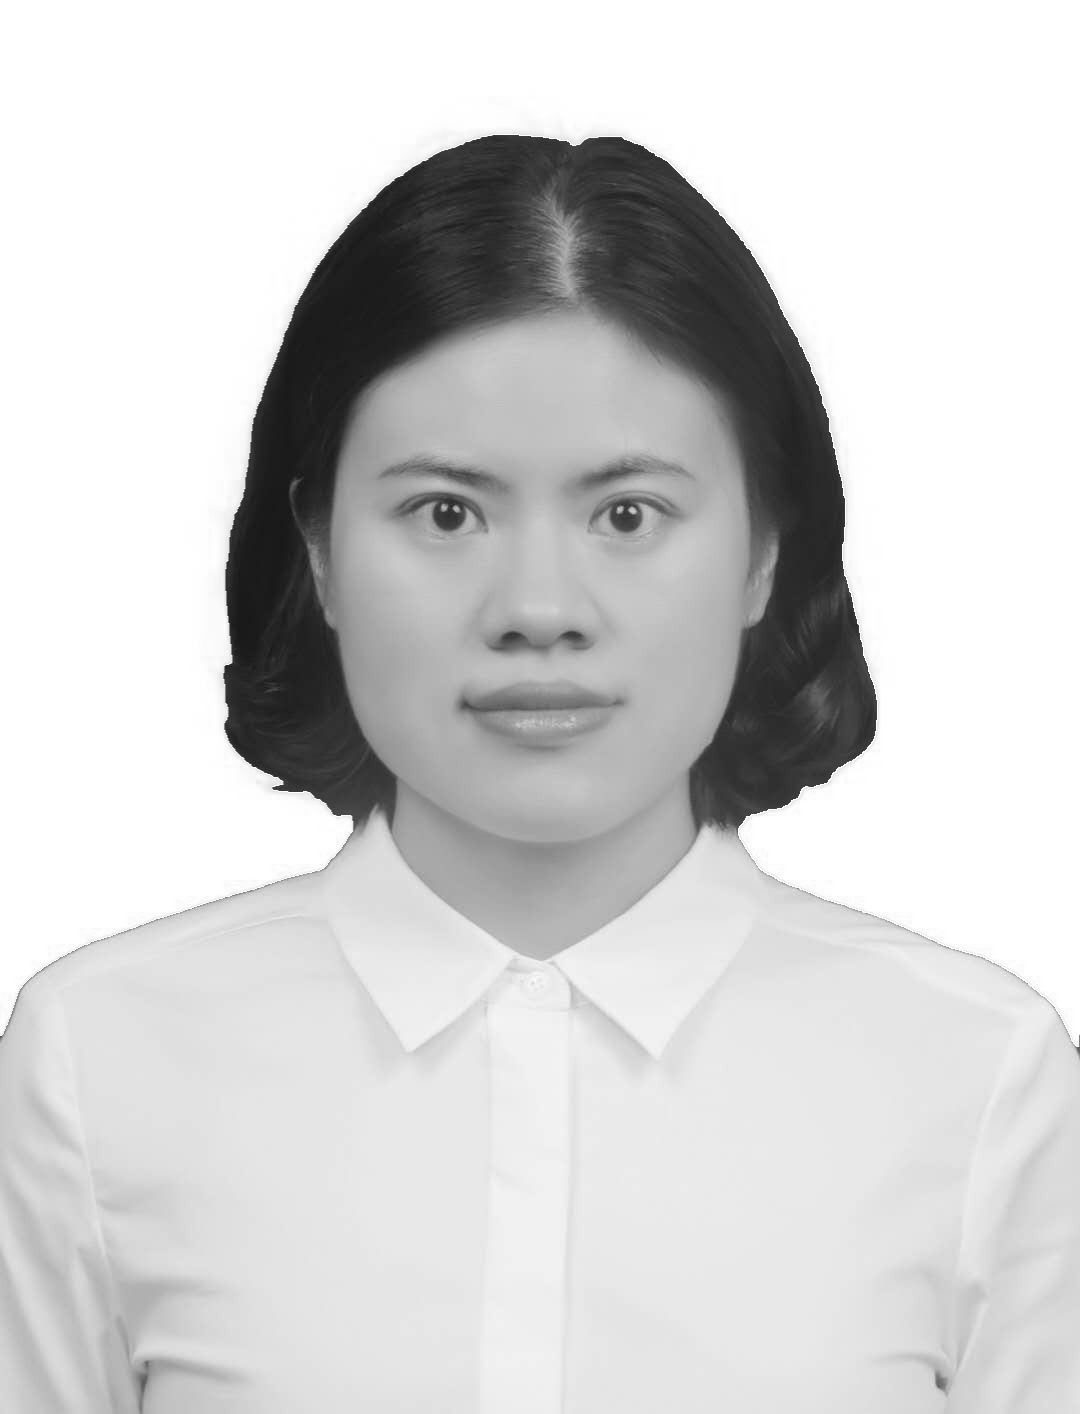
\includegraphics[width=1in,height=1.25in,clip,keepaspectratio]{cf}}]{Feng Chen}
	is a Lecturer in Software Engineering at Chongqing University of Posts and Telecommunications. She received her Ph.D degree from University of Limerick, Ireland. Her current research interests are empirical software engineering and AI for requirements engineering.
\end{IEEEbiography}


 
\begin{IEEEbiography}[{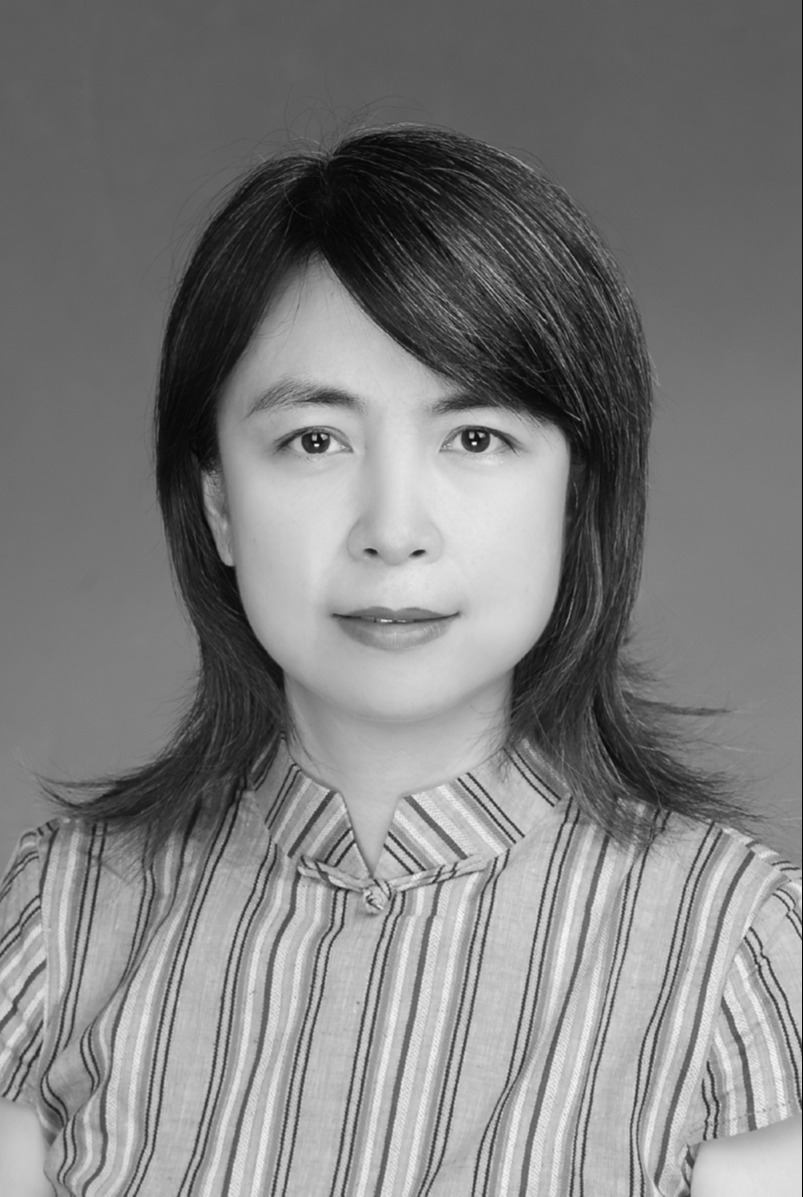
\includegraphics[width=1in,height=1.25in,clip,keepaspectratio]{wqj}}]{Qingjie Wei}
	received her Master’s degree of information science from Kyoto University in 1999. She had worked in IT R\&D Lab of Sumitomo Electric Industries, Ltd. from 1999 to 2004, and won the Best Paper Award for Young Researcher of IPSJ (Information Processing Society of Japan) National Convention in 1999. She is a professor in School of Computer Science and Technology, Chongqing University of Posts and Telecommunications. Her research interests include data mining and process mining.
\end{IEEEbiography}



\begin{IEEEbiography}[{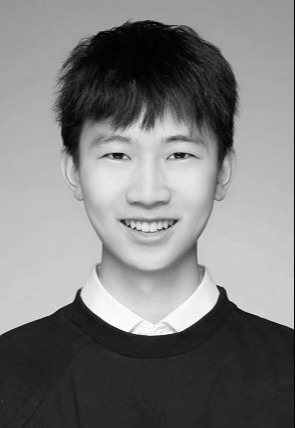
\includegraphics[width=1in,height=1.25in,clip,keepaspectratio]{hhx}}]{Hangxuan He}
	received the BS degree from the Shanghai University of Electric Power, Shanghai, China, in 2022. He is currently working toward the master's degree with Chongqing University of Posts and Telecommunications, Chongqing, China. His reseach interests include federated learning, machine learning, data mining, and data analysis, etc. 
\end{IEEEbiography}

\begin{IEEEbiography}[{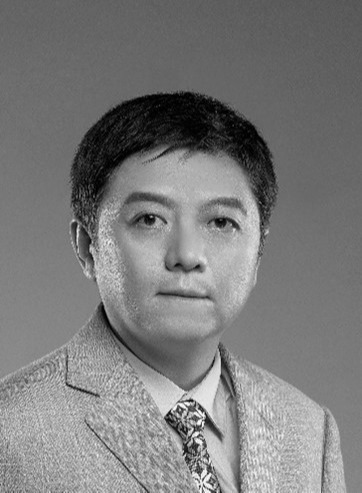
\includegraphics[width=1in,height=1.25in,clip,keepaspectratio]{ying}}]{Ying QIAN}
	received the bachelor’s degree in the Department of Optoelectronic Precision Instruments from Chongqing University in 1990, and the Master’s degree and Ph.D degree in the Research Division in Informatics, Systems Science Course of the Postgraduate School from Kyoto University, Japan, in 1996 and 2000, respectively. In 2000, he joined Mitsubishi Electric Advanced Technology Research Institute, Japan, as a scientist. Since Sep. 2007, he has been with the Software Engineering school of Chongqing University of Posts and Communications, China, as a Professor. He current research interests include Image Processing, Imaging Technology, Software Engineering and Machine Learning Algorithms. He is a member of the IEEE and IEEE Computer, IEEE EMB society.
\end{IEEEbiography}



\end{document}


